\documentclass[UKenglish]{DUO/ifimaster}  %% ... or USenglish or norsk or nynorsk
%\usepackage[UKenglish]{uiomasterfp/uiomasterfp}
%\documentclass[UKenglish]{report}
\usepackage[UKenglish]{uiomasterfp/uiomasterfp}

\usepackage[utf8]{inputenc}           %% ... or latin1
\usepackage[T1]{fontenc,url}
\urlstyle{sf}
\usepackage{babel,textcomp,csquotes,DUO/duomasterforside,varioref,graphicx}
\usepackage[backend=biber,style=numeric-comp,sorting=none]{biblatex}
\usepackage{amsmath,amssymb,amsfonts}
\usepackage{algorithmic}
\usepackage{textcomp}
\usepackage{xcolor}
\usepackage{textgreek}
\usepackage{float}
\usepackage{graphicx}
\usepackage{titlesec}
\usepackage{glossaries-extra}
\usepackage{verbatim}
\raggedbottom %%reduces the gaps between the paragraphs

%\title{Thesis Title}        %% ... or whatever
%\subtitle{A subtitle of your thesis }         %% ... if any
%\author{Emil Christopher Gjøstøl Strømsvåg}                      %% ... or whoever 

\setabbreviationstyle[acronym]{long-short}

\addbibresource{bibliography.bib}            %% ... or whatever
\usepackage{glossaries-extra}
\setabbreviationstyle[acronym]{long-short}


\newacronym{cnn}{CNN}{Convolutional Neural Network}
\newacronym{rnn}{RNN}{Recurrent Neural Network}
\newacronym{cpu}{CPU}{Central Processing Unit}
\newacronym{gpu}{GPU}{Graphics Processing Unit}
\newacronym{vqa}{VQA}{Visual Question Answering}
\newacronym{xai}{XAI}{Explainable Artificial Intelligence} % Should it be Explainable or eXplainable?
\newacronym{ai}{AI}{Artificial Intelligence}
\newacronym{ml}{ML}{Machine Learning}
\newacronym{shap}{SHAP}{SHapley Additive exPlanations}
\newacronym{lime}{LIME}{Local Interpretable Model-agnostic Explanations}
\newacronym{knn}{k-NN}{k-Nearest Neighbors}
\newacronym{gradcam}{Grad-CAM}{Gradient-weighted Class Activation Mapping}
\newacronym{flex}{FLEX}{Faithful Linguistic Explanations}
\newacronym{lstm}{LSTM}{Long Short-Term Memory}
\newacronym{sota}{SOTA}{State-of-the-Art}
\newacronym{nlp}{NLP}{Natural Language Processing}
\newacronym{bvlc}{BVLC}{The Berkeley Vision and Learning Center} % Developed Caffe together with BAIR
\newacronym{bair}{BAIR}{Berkeley AI Research} % Developed Caffe together with BVLC
\newacronym{svm}{SVM}{Support Vector Machines}
\newacronym{svd}{SVD}{Singular Value Decomposition}
\newacronym{pca}{PCA}{Principal Component Analysis}
\newacronym{imagenet}{ILSVRC}{ImageNet Large Scale Visual Recognition Challenge}
\newacronym{ann}{ANN}{Artificial Neural Network}
\newacronym{vit}{ViT}{Vision Transformer}
\newacronym{bert}{BERT}{Bidirectional Encoder Representations from Transformers}
\newacronym{bart}{BART}{Bidirectional Auto-Regressive Transformers}
\newacronym{gpt}{GPT}{Generative Pre-trained Transformer}
\newacronym{vram}{VRAM}{Video RAM}
\newacronym{lora}{LoRA}{Low-Rank Adaptation}
\newacronym{llama}{LLaMA}{Large Language Model Meta AI}
\newacronym{llm}{LLM}{Large Language Model}
\newacronym{roi}{ROI}{Region of Interest}
\newacronym{vgg}{VGG}{Visual Geometry Group}
\newacronym{cuda}{CUDA}{Compute Unified Device Architecture}
\newacronym{relu}{ReLU}{Rectified Linear Unit}
\newacronym{sdg}{SDG}{Stochastic Gradient Descent}
\makeglossaries

%\DeclareGraphicsExtensions{.png,.pdf} % Change this before delivering
\DeclareGraphicsExtensions{.pdf,.png} % Change this before delivering


\begin{document}


\uiomasterfp[
    author={Emil Christopher Gjøstøl Strømsvåg}, 
    colour={orange},
    date={Spring 2023},
    program={Informatics: Robotics and Intelligent Systems},
    dept={Department of Informatics},
    fac={Faculty of Mathematics and Natural Sciences},
    supervisors={Andrea Storås\and Michael Riegler\and Kyrre Glette},
    title={Thesis Title},
    subtitle={A subtitle of your thesis},
    image={images/forside_bilde.pdf}
]
%\duoforside[dept={Department of Informatics},   %% ... or your department
%  program={Informatics: Robotics and Intelligent Systems},  %% ... or your programme
%  long]                                        %% ... or long





\frontmatter{}
\chapter*{Abstract}                
\label{sec:abstract}

\begin{comment}
The abstract is often the first text the reader looks at. Thus, it should be very well written, concise and to-the-point - with the focus of SELLING your work. It is therefore often written at the very end, when you have all details of your work. Usually, we recommend something like this: i) A sentence or three about the background of the challenge you are addressing, which then leads to your “problem statement” (written as just a sentence); ii) Some text describing what you have done in your research, what have you developed, etc.; iii) A small overview of your main results and conclusions - what are the main take-aways from your thesis.

Note also that the abstract is a teaser, and it should therefore not be too long: Fast to read, fast to get to the point. We often recommend keeping it on one page.
\end{comment}


% More complex models
With the increase in accuracy and usability of deep neural networks, there has been a big demand for using these neural networks in different domains to increase productivity, create new industries, and improve people's lives. 
However, these networks are often large and complex, which does not give insight into the prediction process done by the model. 
In order to make the models more functional and be able to improve them, humans need to understand how they reason. 

This thesis will explore image captioning systems that are locally faithful to the underlying method using gradient activations in the network combined with a language model trained on open-ended questions and answers.
\tableofcontents{}
\listoffigures{}
\listoftables{}
% Print Acronyms 
\printglossary[type=\acronymtype, title=List of Acronyms]



%\onehalfspacing
\singlespacing

\chapter*{Preface}                  
\label{sec:preface}

\begin{comment}
Foreword / Preface / Acknowledgements
This is the place for "informal chat" like how the master thesis task has progressed and acknowledgment to those who one feels for thanking. One can also include what kind of software that has been used in the master thesis work. Some choose to have the foreword before the Table of Contents (TOC).
\end{comment}
% Takk til veiledere
I want to thank my supervisors, Andrea Storås, Michael Riegler, and Kyrre Glette, for all your help, motivation, and interesting discussions.
I am thankful that it was you guys that followed me on this journey – without your encouraging presence, this project would not be the same.

% Takk til folk og ML-nodene 
All the experiments conducted during this work have been run on the machine learning nodes at the AI HUB hosted at the University of Oslo. These are now becoming a part of the Norwegian AI Cloud (NAIC). 
Therefore, I would like to thank these nodes for their service, and may you have a prosperous life serving new and interesting assignments.

% Takk til AI-generert forsidebilde
The header image of the cute robot on the front page is made with the help of the generative text-to-image model Stable Diffusion. The image is meant to illustrate a large language model, reading lots of books to gain knowledge. It is wonderful to live in a time where a stressed student can make a beautiful image without having any artistic qualities.


% Hva jeg har lært
This thesis has introduced me to the depths of a very fascinating field of research.
The field of AI and XAI is developing at an extraordinary speed, which is both exciting and important to be aware of, and I am curious to follow the coming advancements. 
Open-sourced AI methods have been essential during the development of this work.

Astonishing advancements are now made in both AI and XAI, and their discoveries help contribute to further democratizing these helpful tools. It is beneficial for interested individuals like me to have models and documentation openly available, and it contributes to the transparency of the extreme advancement.

% Takk til venner og familie og Vics
I want to give a special thanks to all the lovely people at Blindern Studenterhjem. You have given me the best student experience that I could ever dream of. 
Last but certainly not least, I would like to give a huge printed hug to my family and Victoria for motivating me and supporting me throughout this entire voyage.

\mainmatter{}



\chapter{Introduction}               
\label{sec:1_Introduction_all_content}

\label{sec:1_1_background_and_motivation}

\begin{comment}
In about a page, summarize the most important background information. The text usually leads to YOUR PROBLEM STATEMENT (in the next section) and gives arguments about why this is a challenge today.
\end{comment}

\section{Background and Motivation}


% Short description of the problem
    % Deployments of AI more widespread 
    \gls{ai} have made remarkable achievements in various fields, but their lack of interpretability and opacity have brought the question of trustworthiness to the forefront of discussion. 
    % Complex and opaque AI systems that are difficult to interpret
    The black-box nature of \gls{ai} models inhibits user trust and understanding, which can be critical in decision-making scenarios and deploying models in real-world applications. This lack of transparency limits the ability to address bias, identify model limitations, and provide accountability. 


% Short intro to XAI

    % What it is
    \gls{xai} is both a research area and a set of techniques to address these weaknesses by providing methods and techniques to explain the decisions and predictions made by \gls{ai} models.     
    Motivation for \gls{xai} methods arises from the increased deployment of \gls{ai} systems, especially in high-stakes domains such as finance, criminal justice, and healthcare, where justification is vital.
    %These domains need to trust and understand the decisions made to deploy the methods safely and ethically. 
    Additionally, \gls{xai} is important in consumer-facing decision-making applications using \gls{ai}, where users may not have the technical expertise to understand the inner workings of an \gls{ai} system. 
   


% Short intro to VQA
    % What it is
    As many \gls{xai} methods strive to provide locally accurate explanations, that is, explanations faithful to the underlying model, they often include low-level features \cite{dasOpportunitiesChallengesExplainable2020a}. However, often these features are challenging to convey to a non-technical user or do not provide an intuitive explanation. 
    A user can gain a fuller picture of a model's reasoning by having higher-level explanations that come from multiple modalities \cite{alipourStudyMultimodalInteractive2020}.
    The multimodal task of \gls{vqa} combines text questions in natural language and corresponding images to get a model to output a response based on these two modalities. These multimodal tasks are closely related to human cognition, as understanding and describing visual scenes with language is a fundamental attribute of human perception. 
    
    
    % A specific area of \gls{ai} that has received considerable attention is \gls{nlp}, image captioning \cite{vinyalsShowTellNeural2015, youImageCaptioningSemantic2016, vinyalsShowTellLessons2017}, and \gls{vqa}. Image captioning involves generating natural language explanations for visual input, such as images. These tasks are challenging objectives as they require a deep understanding of visual and linguistic information and the combination of these modalities into insight. Explanations are most valuable when they both naturally make sense in the given context and are helpful in their respective tasks.

    
    
    % Research on \gls{vqa} and image captioning has important implications for a variety of applications. For example, in computer vision, \gls{vqa} can be utilized to improve object recognition and scene understanding. \gls{nlp} applications can use information in \gls{vqa} and image captions to improve machine understanding of text and images. This improvement can come from understanding modalities like vision and language to learning visual semantics that better correlate with human thinking. Through cross-modality learning, particularly in the areas of vision and language, like \gls{vqa}, improvements can be made by automating data set generation. Images can be automatically categorized, labeled, and annotated by an \gls{ai} \cite{lancasterAutomatedLabelingHuman1997, mnihMachineLearningAerial}. Models and methods can extract new knowledge about images and videos, like the semi-supervised teacher-student framework proposed by Gjestang et al. \cite{gjestangSelflearningTeacherstudentFramework2021}. In addition, \gls{vqa} and image captions can also be applied to assistive technologies, such as helping visually impaired people understand and navigate their situation or helping robots understand and react to their surroundings.

% Connect XAI and VQA

    The combination of the \gls{vqa} task and \gls{xai} is an important area of research since it has the potential to bring the most intuitive explanations to researchers and users. By describing the contents of images in natural language and being able to answer questions regarding images and text, users can gain a better insight into these complex models and determine if they can be trusted in critical assignments. 
    
    % How it can make a difference
    % The importance of \gls{xai}, \gls{vqa}, and image captions is further reinforced by recent advances in deep learning and computer vision, as these techniques have greatly improved the performance of \gls{xai} systems in these tasks. However, despite these advances, many challenges remain to be addressed, such as the lack of interpretability of deep neural networks. Solving these challenges and advancing the state-of-the-art in \gls{xai} and \gls{vqa} are important research goals that can lead to significant advances and deployments of \gls{ai} systems.

% What this work is and solves these problems
    This work explores how \gls{vqa} systems can be explained using visual and linguistic justifications. As complex models often achieve the highest accuracies, the experiments in this work explore how smaller, transparent, and explainable methods can be attached to a fully developed primary model. These models can provide valuable insights during development and in the real world at no cost to the predicting model's accuracy.
        
     % How it can make a difference
    %\gls{xai} aims to make \gls{ai} systems more interpretable, intuitive, and trustworthy by generating explanations that are descriptive, faithful, and understandable to humans. These explanations help users understand the reasons behind \gls{ai} decisions, uncover bias, assess trustworthiness, and identify potential areas for improvement.

% Summary that leads to the problem statement
%In summary, \gls{xai}, \gls{vqa}, and image captioning are important research areas that have many real-world applications and implications. These tasks are challenging and require a deep understanding of both visual and verbal information. Both of these areas can lead to significant advances in \gls{ai} and \gls{xai}. Making these models more reliable and trustworthy for use in high-stakes scenarios and more accessible to everyday users with no domain knowledge. Research in these areas will also benefit from advances in deep learning and computer vision. Likewise, research on interpretability issues must be done.
\label{sec:1_2_problem_statement}

\begin{comment}
In a short and precise way, state what your research is about in this thesis. It can be in the form of a (set of) research questions, goals/aims, or objectives (or a mix) - but it should clearly state what the problems or challenges you are addressing.

Alternatively, one can state a research hypothesis, but if so, it should follow the rules of what a hypothesis is. A hypothesis is a statement that introduces a research question and proposes an expected result. It is an integral part of the scientific method that forms the basis of scientific experiments. Therefore, you need to be careful and thorough when building your hypothesis, following the “rules”.
\end{comment}

\section{Problem statement}

% Intro
For machine learning and computer vision to be truly trustworthy, they will need to be understood. Researchers need to understand the inner workings of the model to improve it and discover biases in the dataset. Users and domain experts utilizing the models need to have trust in the model predicting accurately while using useful features when evaluating. The models should be able to achieve \gls{sota} performance, without sacrificing interpretability and explainability in what they evaluate when predicting. 

% What this is and How I want to do it
In this thesis, the goal is to explore the roam of visual and linguistic understanding.
The visual knowledge will come from a \gls{cnn} that learns features in images. An \gls{rnn} \cite{rumelhartLearningRepresentationsBackpropagating1986, choLearningPhraseRepresentations2014, sutskeverSequenceSequenceLearning2014, bahdanauNeuralMachineTranslation2016} or transformer is used to extract linguistic information from open-ended questions and answers in natural language, taken from a \gls{vqa} dataset. A backward pass that looks for large gradients through layers of the \gls{cnn} will be used to choose locally faithful words to caption the image in an explainable way. 



% Questions to be answered
The main topics that will be explored to reach the research goal are: 
\begin{itemize}
    \item Does an explainable image caption model improve its answers when trained on a \gls{vqa} dataset?
    \item With only the explaining model choosing the captions, will the output be more intuitive for humans?
    \item Are the explanations, both captions, and answers from open-ended questions locally faithful to the underlying \gls{cnn} model?
    \item If there is enough time during this thesis, it would be an interesting task to see if the image caption and \gls{vqa} will perform better when using transfer learning  on a language model pretrained on a large language dataset. 
\end{itemize}

% What is the result
With these research questions answered, this thesis will be one step closer to an explanatory model that can give insight into how models understand broad concepts in vision and language. This knowledge can be used to make computers understand a more complex worldview and help humans understand what it sees and value.

\subsection{Proposed architecture}
Figure \ref{fig:architecture_proposal} shows how the data flow in the proposed method can work. It closely follows the \gls{flex} \cite{wickramanayakeFLEXFaithfulLinguistic2019} architecture proposed by Wickramanayake et al. It consists of a \gls{cnn} that extracts visual information and a 2-layered \gls{lstm} \cite{hochreiterLongShorttermMemory1997} \gls{rnn} that combine linguistic information with extracted visual features. The reason why this architecture is relevant for this thesis is that it uses a backward pass to find locally accurate visual features, which are then used to give an image caption that describes what visual features actually were important to the classification and captioning of the image. This makes the architecture useful as a starting point for this thesis and can be adapted to use \gls{vqa} datasets as linguistic input, to make it possible to ask questions regarding the classification of images and predictions. 

% Explain the proposed data flow / architecture 
    % Training
    % CNN
During training the proposed architecture takes an image and its corresponding questions and answers from the \gls{vqa} dataset. The images are fed through a \gls{cnn}-network, which can be pretrained on a larger dataset, like ImageNet \cite{dengImageNetLargeScaleHierarchical2009}. This is because the explaining method utilizes feature maps in each layer of the \gls{cnn}, so it is agnostic on what type of \gls{cnn} it is and what dataset it is trained on earlier. The \gls{cnn} predicts a class of what it sees in the image, and with a backward pass, finds important feature maps in each  convolutional layer. Each feature in the set of important feature maps gets associated with a word and stored in a relevance vector. This process is done by computing a co-occurrence score between each word in the ground truth caption and the feature. The feature with the highest co-occurrence score gets linked with that feature. 

    % LSTM
The \glspl{lstm} gets trained by feeding each word in the ground truth caption into the first layer, alongside the hidden state of the \gls{lstm}. This is used to compute the next state, which gets concatenated with important visual features, and is input to the second, and last, \gls{lstm}-layer. 
The output from the second \gls{lstm}-layer is encoded to vocabulary space that is used to make a conditional probability distribution that later will be used to calculate the probability for predicting that word, given the given image features. 

    % Testing
During prediction, the architecture takes an image and an optional question as input. The \gls{cnn} extracts important features in the layers, which get fed into the \gls{lstm}. Important feature maps from the \gls{cnn} are also used to calculate the relevance vector between features in the image and words. The \gls{lstm} uses this relevance vector, alongside important decision-relevant features from the image to predict a word. This word prediction is repeated until the stop word is predicted. 

If no question is input to the algorithm during prediction, the model will use the most accurate predicted answer caption that describe the image as a whole as a caption for the image. On the other hand, if a question is submitted alongside the image, the \gls{lstm} will generate captions that answer the question asked, and then choose the most decision-relevant answer as the caption. 



% Data flow
\begin{figure}[htb]
    \centering
    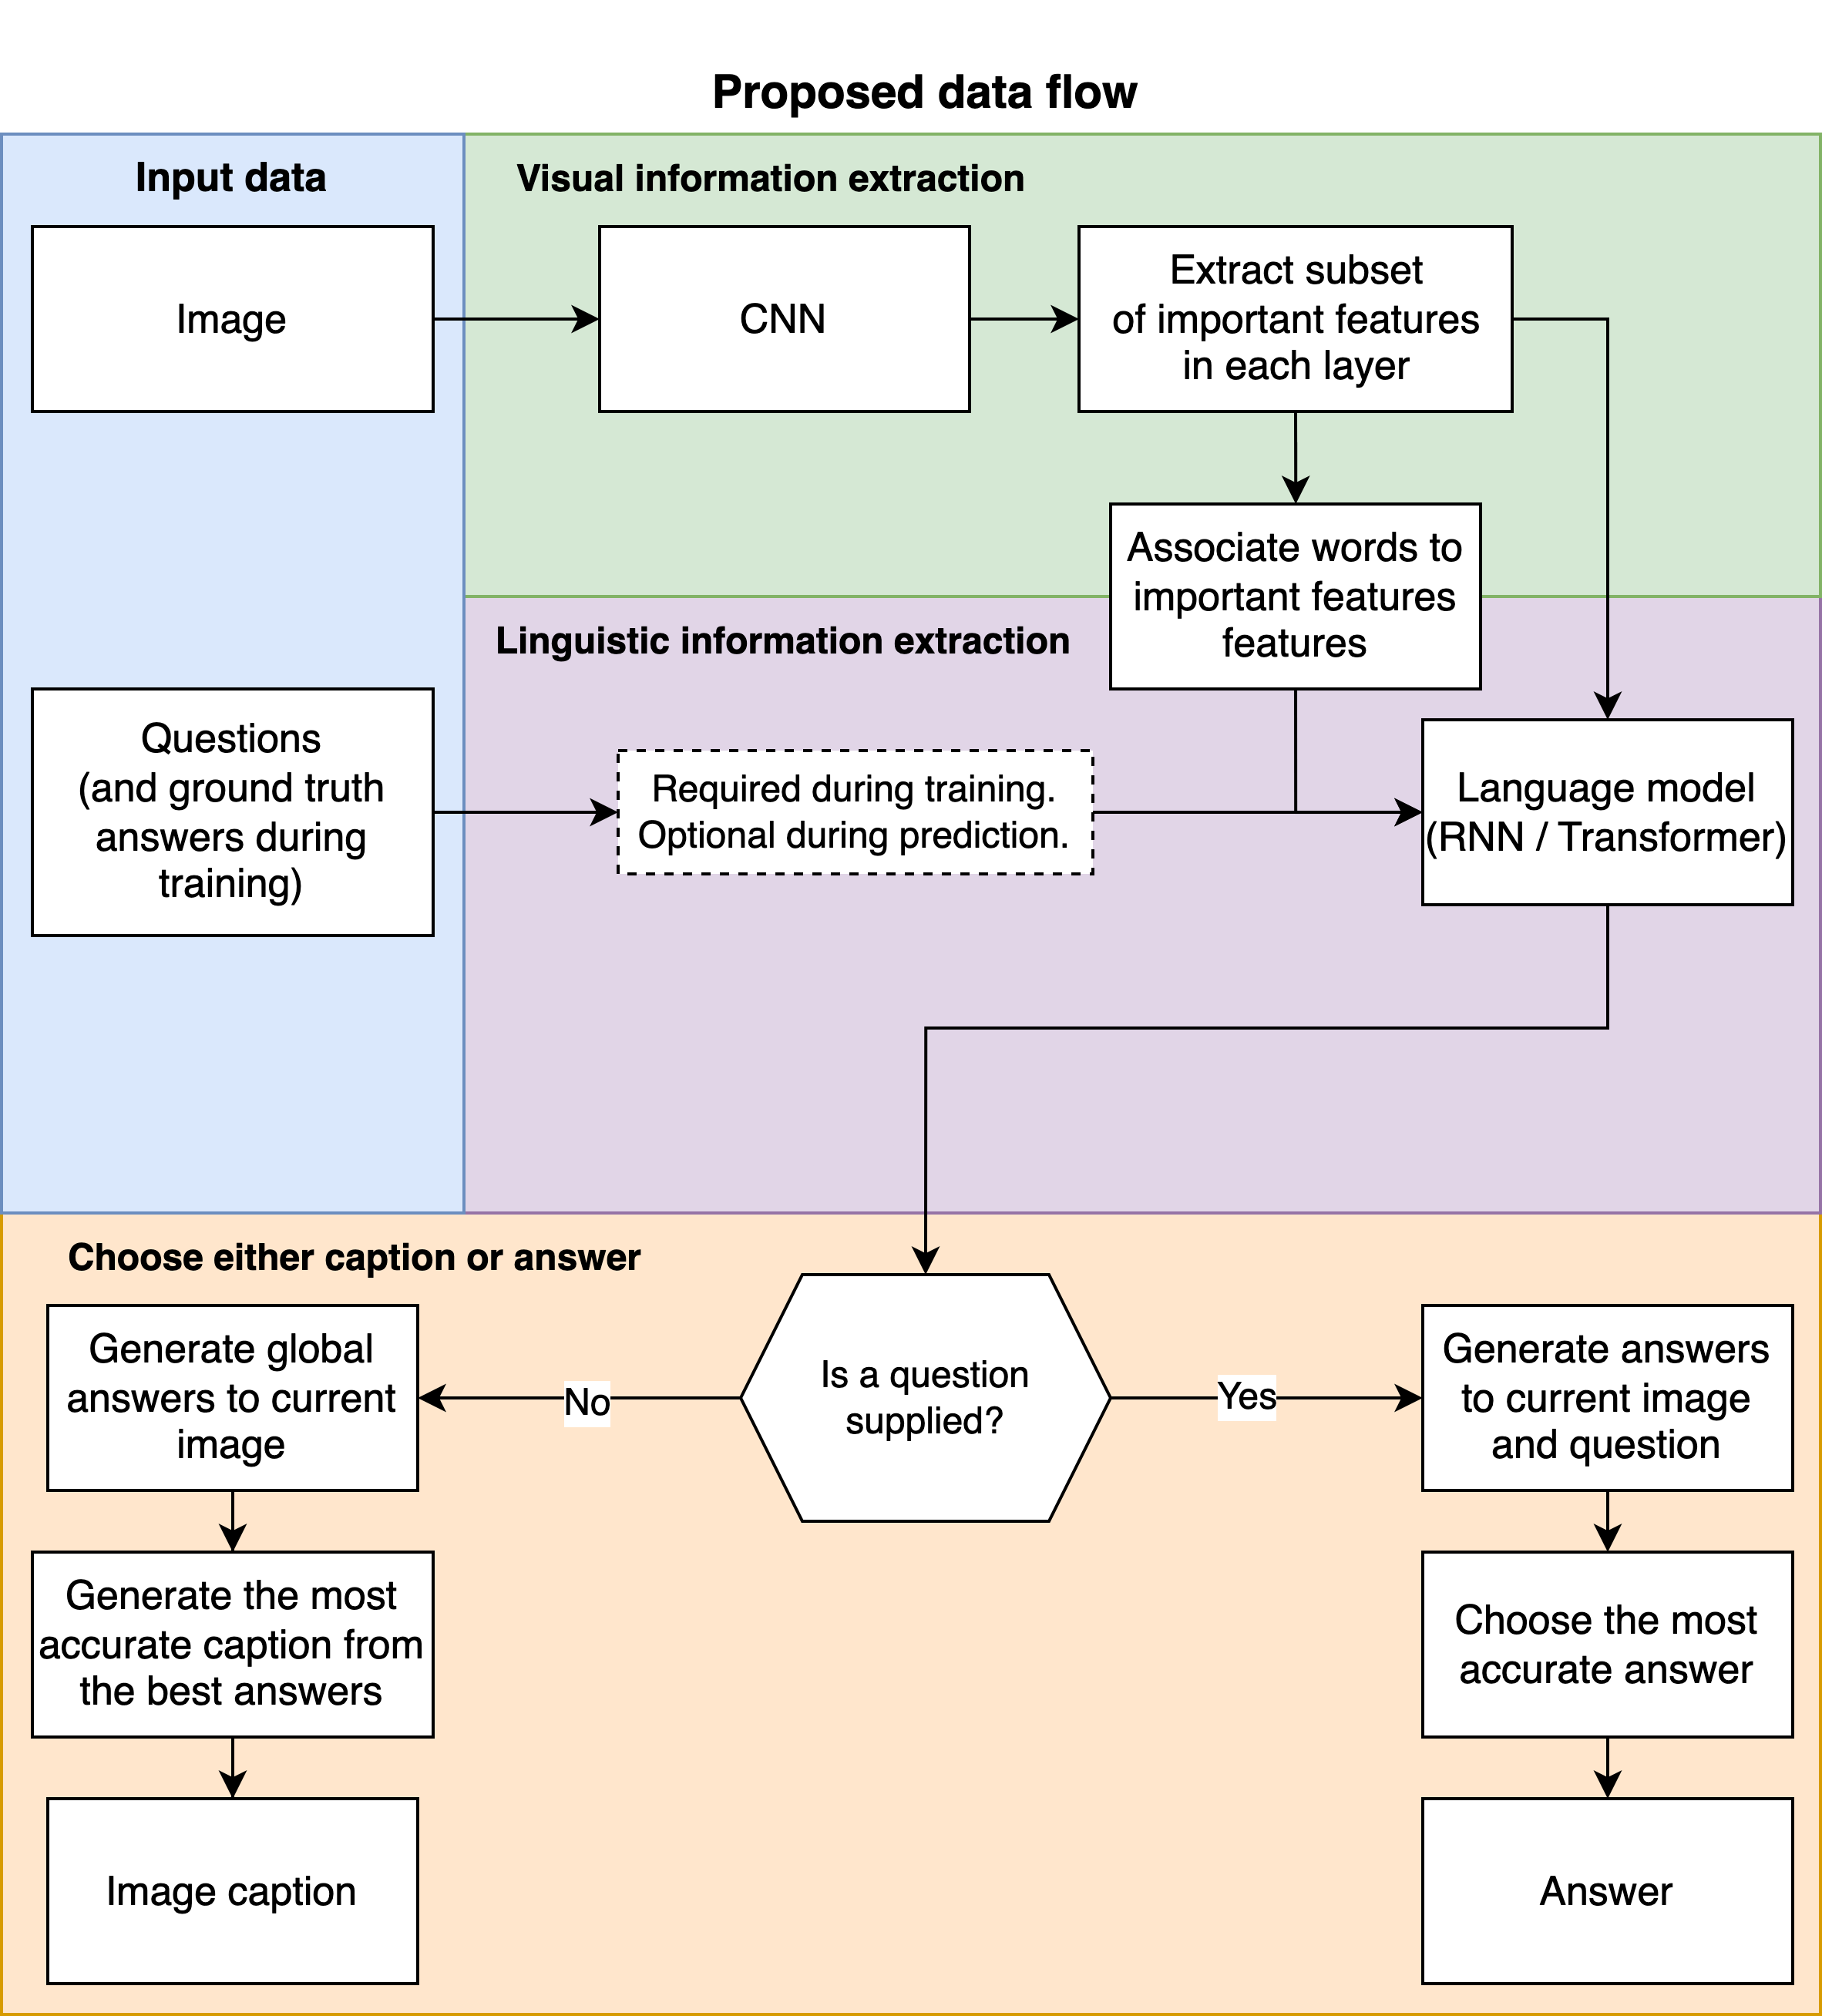
\includegraphics[width=12cm]{images/architecture_proposal.png}
    \caption{Proposal of the data flow and components that will be explored in this thesis.}
    \label{fig:architecture_proposal}
\end{figure}
\label{sec:1_3_scope_and_limitations}

\begin{comment}
Here you can tell the reader about the scope of your thesis, kind of meaning describing what you have done in slighter more detail. The question in section 1.2 might be of the general type, but are you using any specific case studies/application scenarios? Are you limited to a specific type of platform? Have you performed experiments in special environments only, etc.? Describe such information here so that the reader does not expect something going beyond this.
\end{comment}

\section{Scope and limitations}

% Scope:

    % Run on VQA 2.0 dataset 

    % Run with VGG-16





% Limitations:

    % Only with one CNN (VGG16 and Compact Bilinear Pooling)
    
    
    % Only on VQA 2.0 dataset
    
    
    % Only compared to the algorithm in the VQA 2.0 paper and regular image captionings. 


    % Using Caffe
    

\label{sec:1_4_research_methods}

\begin{comment}
You are doing a research education, so it might be nice to show that you are aware of different ways of doing research. Here, you should describe your research methods showing the reader that you are conscious of your method. There exist several methodologies, and finding a reference somewhere would probably be good.
\end{comment}

\section{Research methods}

In order to answer the research goals and achieve the goal of this thesis, a proof of concept method was developed and implemented by the author. In order to have an implementation the new method could be tested against, an existing code base was used as chosen as a starting point. The most fitting existing method was \gls{flex} \cite{wickramanayakeFLEXFaithfulLinguistic2019}. 

The reason why this method was chosen was that it proposes a novel method to associate features responsible for the decisions in a \gls{cnn} model with words. This way it can generate intuitive, descriptive and faithful explanations that annotate objects in an image. These post-hoc justifications for classification using natural language is achieved using a \gls{cnn} for extracting features in images and two stacked \glspl{lstm} to extract features from text descriptions during training phase, and use this knowledge and \glspl{lstm}, in conjunction with image features to give faithful descriptions during testing, when no text descriptions is supplied with the image.


\label{sec:1_5_ethical_considerations}

\begin{comment}
Ethical considerations in research are a set of principles that guide your research designs and practices. Scientists and researchers must always adhere to a certain code of conduct when collecting data from people. For example, the goals of human research often include understanding real-life phenomena, studying effective treatments, investigating behaviors, and improving lives in other ways. What you decide to research and how you conduct that research involve key ethical considerations such as:

i) protect the rights of research participants (privacy); 
ii) enhance research validity, 
iii) maintain scientific integrity; etc. Thus include here a short description of an assessment of any relevant potential ethical considerations.
\end{comment}

\section{Ethical Considerations}



% Into and identify bias (main)
With more intuitive explanations provided by an \gls{xai} system, researchers and users have better insight into the inner workings and arguments of the underlying \gls{ai} method. This, in turn, will address one of the ethical concerns, which is dataset bias. 

\subsubsection{Dataset Bias}
\gls{ai} raises a number of ethical concerns, particularly when used in high-stakes domains such as healthcare, finance, and criminal justice. The concern is not specifically the error of the \gls{ai} model but rather the bias of datasets. Since \gls{ai} is used to condense complex datasets into understandable predictions, it becomes an inherited ethical issue if models learn unfair biases. 
Datasets used in deep learning are often large and complex, and \gls{ai} models are used to extract knowledge from the dataset. Therefore, it can be difficult for researchers and users to identify biases used in training the \gls{ai} models, especially when they do not explain why this prediction is correct. 

% Example of bias in prediction
One ethical problem is that \gls{ai} systems can make predictions that are directed against certain groups of people, such as those from marginalized communities. This could occur if the training data used to develop the system is biased or if the system's decision-making process is not transparent. \gls{xai} can therefore be an important tool to gain insights into our own biases and to help researchers and users avoid making decisions based on false premises. 


% Another ethical issue with \gls{xai} is the possibility that the system will be used for surveillance or other privacy-intrusive purposes. For example, an \gls{xai} system used to monitor people in public spaces could raise concerns about civil liberties and privacy rights. In addition, \gls{xai} systems capable of understanding and interpreting visual or textual information could also be used to profile individuals based on their race, gender, age, or other personal characteristics.



% Bias in VQA
\gls{vqa} datasets and image caption tasks also raise ethical concerns about bias and fairness. The task of \gls{vqa} and image caption rely on data in order to learn to generate textual explanations for visual inputs. However, if the training data is biased in any way, the resulting system will also be biased. For example, if a \gls{vqa} dataset contains mostly humans with one skin color, the system may not work as well with images of people of a different color. 
Similarly, if a dataset used for captioning contains a relationship between sexes and professions, the same bias will be carried over to the model.

% Another ethical issue related to \gls{vqa} and captions is the potential of the generated captions and explanations to perpetuate stereotypes or reinforce societal prejudice. For example, if a system is trained on images that portray people of a certain gender or race in a certain way, it can generate captions that perpetuate those stereotypes. In addition, when used in certain applications, such as facial recognition, the system could reinforce societal prejudice and perpetuate discrimination.

% How VQA bias can be mitigated
The work of Hirota et al. \cite{hirotaGenderRacialBias2022} analyzed gender and racial bias in five popular \gls{vqa} datasets and found unfavorable stereotypes in the samples. 
Various possible solutions to address this issue were explored in their work.
This includes not asking questions about race and sex when not required when making a dataset and collecting a more standardized distribution related to race and sex. 
They also propose an alternative to the manual screening that some \gls{vqa} datasets use since not all can justify the cost of manual annotation. The proposed solution to this automatic screening, followed by ethical guidance for annotators, and lastly, a feedback platform for users.


% LLM
\subsubsection{Large Language Models}
Regarding \glspl{llm}, there are some ethical considerations to address. \glspl{llm} are trained on a large corpus of text, most often collected from the Internet. The data gathered across the web are mostly written by humans, and the \glspl{llm} are trained on this wast dataset to extract a more general understanding of human knowledge and present this with a well-structured syntax. With the advancements and availability of models such as \gls{gpt}-4 \cite{openaiGPT4TechnicalReport2023}, combined with a user-friendly and easy-to-use user interface, like the one used by ChatGPT \cite{ChatGPT}, the public has never before had an advanced \gls{ai} so accessible in their everyday life. Given that users come from different backgrounds and cultures, the \gls{llm} should be able to adapt to its users to close the gap between user and \gls{ai} alignment. 
% something about the alignment problem.
\gls{ai} alignment is a subfield of \gls{ai} safety, with the goal of building safe and reliable \gls{ai} methods \cite{amodeiConcreteProblemsAI2016}. 
% Inner and outer alignment
The alignment problem is defined as the task of aligning the goals of the humans creating the system with the goals of the \gls{ai} system. Outer alignment is the overall goal of the system, and inner alignment ensures that the system behaves as expected in a robust manner \cite{ngoAlignmentProblemDeep2023}.

% Something about hallucinations

\glspl{llm} have billions of parameters and incomprehensible feature space for humans to understand fully. These models are mostly built today using the Transformer model proposed by Vaswani et al. \cite{vaswaniAttentionAllYou2017}, but because of their size and scale, they are very complex to understand \cite{liptonMythosModelInterpretability2017a}. 


% Lex Podcast with Sam
% Sam Altman, the founder and CEO of OpenAI, has in an interview said that solving the alignment problem in \glspl{llm} is not a separate task from improving the model, but solving the alignment problem will also make the models better and more usable for researchers and users. This statement is backed by research, from among other ??? and ???. Solving the alignment problem will give models that better align with humans' overall goal and have an intrinsic goal of following these goals. This can make models easier to adapt and fine-tune to different specific areas of interest, which also will make them more useful and widespread. 


% The open letter to pause training large models
There have been multiple attempts recently to slow the growth of or to regulate deep neural networks, like \glspl{llm}. The goal of this is to have time to address ethical and technical concerns before a new, larger, and better model gets released \cite{PauseGiantAI, REGULATIONEUROPEANPARLIAMENT2021}. The reasons why some argue not to continually make new models are many, but the most prominent concern is to understand better the models already developed. With a better understanding of these models, researchers are better equipped to tune models to better align with the overall goal of humans. An understanding of the inner workings of a model, including an \gls{llm}, can also give insight into how to make the model predictions more transparent, fair, and efficient. 

Ensuring the ability to detect \gls{ai}-generated content is a crucial aspect that deserves significant attention. As \gls{ai} becomes more proficient at autonomously searching the web and generating new datasets, it becomes increasingly important for humans to determine the origin of information and assess its reliability and credibility. These tools play a crucial role in providing transparency and allow users to differentiate between content generated by humans and \glspl{ai}. By integrating reliable detection tools, individuals can make informed decisions based on awareness of whether the information they encounter comes from \gls{ai} algorithms or human sources.


% Carbon Footprint
\subsubsection{Carbon Footprint}
Training large \gls{ai} models takes a considerable amount of energy and therefore produces a lot of greenhouse emissions.  
In the paper introducing the \gls{llama} model \cite{touvronLLaMAOpenEfficient2023}, which is the base model of the Alpaca-VQA model used in this work, they calculate the carbon footprint. This footprint can be estimated by the formula in \autoref{eq:carbon_footprint}.

\begin{equation}
    \text{Wh} = \text{GPU hours} \times (\text{GPU power consumption}) \times \text{PUE}
    \label{eq:carbon_footprint}
\end{equation}

Where \textit{PUE} is Power Usage Effectiveness, which is set to 1.1.
In order to generalize the carbon footprint, the authors of \gls{llama} use the US national averages carbon intensity factor corresponding to 0.385 kg CO\textsubscript{2}eq/KWh, where CO\textsubscript{2}eq is Carbon Dioxide Equivalents. By generalizing the carbon emissions per watt, it is easier to compare models trained in different locations.
The formula used for calculating the metric tonnes of CO\textsubscript{2}eq can be done with the formula in \autoref{eq:tonnes_co2}.

\begin{equation}
    \text{Metric tonnes of CO\textsubscript{2}eq} = \text{MWh used } \times 0.385 \text{kg CO\textsubscript{2}eq/KWh}
    \label{eq:tonnes_co2}
\end{equation}

 
Following this equation, the researchers estimate the development of \gls{llama} to use 2,638 MW in total, corresponding to 1,015 metric tones of CO\textsubscript{2}eq.
This is roughly the same amount as 216 passenger vehicles emit in a whole year \cite{usepaGreenhouseGasEmissions2016}.

In order to minimize the carbon footprint of the \gls{llm} used in this thesis,
the weights used are not from the original \gls{llama} but from the Stanford Alpaca model. 
The model is fine-tuned using optimizations that freeze the internal weights of the model, and a supplementary weight matrix is trained. This implementation is discussed in further detail in \autoref{sec:3_alpaca_vqa}. Also, the experiments follow an iterative design, which helps reduce unnecessary computing time and emissions.
Following the same formula, the fine-tuning of the Alpaca-VQA model used in this work can be calculated. 
It is estimated that the total \gls{gpu} processing time to be 30 hours, with \glspl{gpu} using a maximum of 250 W \cite{Nvidiaa100datasheet}. Using the same PUE as \gls{llama}, the total power consumption is 7.5 kW. 
Using the carbon emissions from the US, the experiments in this work have emitted 2.888 kg of CO\textsubscript{2}eq. 
However, as the servers were located in Norway, the emissions, in reality, were much less. It is estimated that the average emissions per kWh in Norway in 2022 were 0.019 kg CO\textsubscript{2}eq/KWh \cite{LavtKlimagassutslippKnyttet}. Therefore, the actual emissions are 0.143 kg of CO\textsubscript{2}eq, which is less than a kilometer driven in a fossil car \cite{HvaPavirkerUtslipp2017}.


As the fine-tuning used to conduct the experiments in this work is dependent on the base model, the emissions should therefore be seen in conjunction with the final model. 
Therefore it is an ethical concern to keep making larger models that consume more energy, especially when the energy used is not from renewable sources.


To address the issue of large computational needs, processor designers have made specialized chips for machine learning \cite{byunBenchmarkingDataAnalysis2017, jouppiMotivationEvaluationFirst2018, elsterNvidiaHopperGPU2022, kasperekComparisonUsabilityApple2022}. These can assist the development of even better models that also have reduced power consumption. An additional benefit of having reduced power consumption is that more lightweight devices can train and run models that help democratize machine learning. 






% Transformers output linearly, with no internal dialog (reasoning)

% Models are trained as imitators, humans are good at giving human features to non-humans (anthropomorphism). 

% Reinforcement learning from human feedback (RLHF) teaches models to give answers that the human appreciates and thumbs up, giving an incentive to answer something that the human would like to hear, or harmonizes with the humans' previous beliefs. Truth does not care if the human likes it or not, so giving this incentive would make the model pay less attention to giving correct answers, but rather giving answers humans like. 



% EU - The AI Act

% If humans continue to hype the methods recently proposed, like ChatGPT, but the models do not fulfill the hype, there may be another AI winter. One of the main reasons for the two AI winters, as discussed in context in chapter 2 - is background history.


\begin{comment}
    Tell how this thesis uses the ethical information above when doing research.
\end{comment}

In summary, \gls{ai}, datasets \gls{vqa}, and \glspl{llm} raise important ethical concerns about bias, fairness, and carbon footprint. Mainly these concerns stem from reliance on training data, which may be biased or perpetuate stereotypes. 
Researchers and users of these tools must consider the ethical concerns and work towards developing \gls{xai} systems that are transparent, fair, and respectful of humans and the climate.
\label{sec:1_6_main_contributions}

\begin{comment}
It is important to “sell” your work to the reader, making him interested and impressed with your accomplishments. Thus, you should briefly summarize what you have done, list your main results, drawn conclusions and knowledge gained - and put it back in the context of your problem statement. Show how you solved the initial problem or answered the research questions!
\end{comment}

\section{Main Contributions}


\label{sec:1_7_thesis_outline}

\begin{comment}
Describe how you have divided your thesis into chapters, and briefly list what the reader will find in each chapter.
\end{comment}

\section{Thesis Outline}

This work is divided into five main chapters.
All the references used are listed after the last chapter. 
The thesis is structured in the following way:

\begin{itemize}

    \item \textbf{Chapter 1: Introduction} - This is the introduction to this project and thesis. It is designed to be intuitive to follow and convey this research project's motivation and overall goal.
    
    \item \textbf{Chapter 2: Background} - This chapter establishes the foundation and context for the subsequent thesis chapters. It provides the necessary background knowledge and related work for understanding the research conducted in this thesis. It covers the motivation for the research, the importance of XAI, relevant technologies such as AI and machine learning, model explanation techniques, evaluation metrics, and a summary of related work in the XAI field.
    
    \item \textbf{Chapter 3: Methodology} - This chapter delves into the details of two proposed methods in this work, both aiming to explore the implementation of explanatory methods in different domains using machine learning models. The first method, FLEX-VQA, combines a \gls{vqa} architecture with the \gls{flex} framework to provide explanations originating from the visual domain translated into natural language. The second method involves an \gls{llm} combined with a \gls{cnn}, where image features are translated into text for explanation. 
    The chapter highlights the significance of these models' multimodal capabilities and discusses the specific techniques employed. The Alpaca-VQA model, chosen for its pre-training and efficiency, is fine-tuned using the LoRA technique.

    
    \item \textbf{Chapter 4: Experiments and Results} - In this chapter, the Alpaca-VQA model is tested on two different dataset sizes, starting with an investigatory experiment on a smaller dataset to gain initial insights. The model is then trained on a larger dataset of 20,000 samples, and the results are analyzed. Using explanatory post-hoc methods, such as a proxy model explained by \gls{lime} and visualizing transition scores, uncovers biases in the dataset and provides supplementary information about the model's behavior. The chapter also explores linguistic biases by testing a language-only version of the model. The key takeaway is that smaller explanatory methods can be added to larger models after training, providing valuable insights without compromising accuracy or computational resources.
    
    \item \textbf{Chapter 5: Conclusions} - This chapter concludes this thesis and summarizes the findings from the previous chapter. Limitations of the methods used are discussed, as well as future works are suggested. 

\end{itemize}





\chapter{Background}
\label{sec:2_background_all_content}

\label{sec:2_background_theory}


% Broader picture
\section{Artificial Intelligence}

% Short intro
\gls{ai} is both a research topic and a group of approaches aimed at giving computer programs the most intelligent possible approach to solving a given task. In academia, it became a research topic in 1956 after a conference called the Summer Research Project on Artificial Intelligence, which was hosted by John McCarthy and Marvin Minsky, which is considered to be where the term originated and is often credited to McCarthy \cite{mccarthyProposalDartmouthSummer2006, andresenJohnMcCarthyFather2002}. Since this first conference, the field has evolved with the help of an interdisciplinary environment of computer science, mathematics, statistics, psychology, neurology, and linguistics.

% What this section is about
Overall, this section of the thesis provides a brief overview of the history of AI and sheds light on the importance of the field in modern society. It forms the basis for the further discussion of relevant AI concepts in the following sections of this work.

Throughout history, humans have had the desire to wield the power of creating artificial creatures. The concept of artificial beings that are able to observe, evaluate and react to their surroundings can be dated back to the story of Talos in Greek mythology \cite{universityAncientMythsReveal2019}. The concept has since been featured in countless fiction novels and movies, such as Frankenstein, R.U.R, HAL9000, and Metropolis \cite{shelleyFrankensteinModernPrometheus1992, capekRossumUniversalRobots, kubrick2001SpaceOdyssey1969, langMetropolis1927a}. 

Humanity has since taken the dream of artificial beings with consciousness from the realm of fiction and driven the evolution of \gls{ai} as a research field forward with impressive results. 
AI has become an integral part of people's everyday lives, fueling advances in science and technology, including social media, computational photography, voice assistants, and chatbots \cite{barbastathisUseDeepLearning, hoyAlexaSiriCortana2018, biswasRoleChatGPT2023}. Doctors can now use \gls{ai} to interpret medical images, and artists are using AI to create new art \cite{wangMachineLearningRadiology2012, thrallArtificialIntelligenceMachine2018}.


\subsection{A Short History of AI}
% Alan Turing 
The origins of modern AI can be traced back to the 1940s and 1950s when pioneers such as Alan Turing and John McCarthy laid the foundations for today's AI research methods. 

Alan Turing was a British mathematician and pioneer of computer science, and he is most notably known for his contributions to the development of modern computer theory. In 1936, Turing presented his theory of computation, which proposed a system later coined as a Turing machine, which is an abstract machine that manipulates a strip of tape using only simple rules. Despite its limited rules, they can be combined to interpret any proposed computer algorithm. The theory was revolutionary at the time and laid the foundation for the development of modern computers and later became known as the Church-Turing thesis \cite{turingSystemsLogicBased1938, churchUnsolvableProblemElementary1936}. 

One of the first to use Turing's theories in practice was McCullough and Pitts and their formal design of artificial neurons in 1943 \cite{mccullochLogicalCalculusIdeas1943, piccininiFirstComputationalTheory2020}, which was the first step towards the method now known as the perceptron. In 1950, Turing proposed a behavioral test, originally called the imitation game and later named the Turing test. This behavioral test was set up so that a human would speak to two separate entities, the human judge knowing that one was another human and the other a machine. Then the human would talk to those two participants, not knowing whether the responder was the human or the machine, and then try to decide who the machine was. The computer would pass the Turing test if the human judge could not distinguish between human and computer. This test is relevant today with tools such as ChatGPT \cite{ChatGPT}, where the boundary between human and machine-produced natural language disappears. Turing's work laid the foundation for modern computers and artificial intelligence. His ideas are still relevant today, and his impact on the field of computer science cannot be overstated. The Church-Turing thesis, in particular, had a significant impact on the research field of studying computers and giving an understanding of the limitations of computer systems. Turing's work also laid the foundation for the development of artificial neural networks and their use in machine learning.

The research field of artificial intelligence has gone through several ups and downs over the years. These ups and downs have mostly been caused by increased popularity and interest in founding new technologies in the field, followed by disappointment when the development didn't deliver the desired results. Disappointment led to cuts in funding, which stagnated development. The AI industry has experienced two significant cycles of reduced interest, often referred to as the two AI winters. The first AI winter was in the late 1970s, and the second was in the late 80s to early 90s \cite{floridiAIItsNew2020}. Since the beginning of 2012, interest in AI has increased, driven in particular by advances in machine learning, deep learning, and increased computing resources. With the advent of deep learning and big data, AI has seen a resurgence, and unprecedented advances have been made in the field in recent years. This has led to the development of intelligent systems that can take on a variety of tasks that were once thought to be an exclusive domain of humans, such as driving cars and interpreting images. 

As there exist many ways to solve a problem, researchers have divided the \gls{ai} field into two main paradigms that take different approaches to achieving artificial models. 
The two paradigms are named symbolic and connectionist \gls{ai}.


% Symbolic artificial intelligence
\subsubsection{Symbolic Artificial Intelligence}


Symbolic Artificial Intelligence refers to a collection of AI methods based on high-level symbolic representation of problems. It is also known as rule-based AI, classic AI, and good old-fashioned AI (GOFA) \cite{haugelandArtificialIntelligenceVery1989}. 

In the period between the 1950s and mid-1990s, symbolic representation was seen as dominant over the other main representation, connectionism, which will be discussed in the next sub-chapter. This was because symbolic representation came closer to the thought human way of learning symbolic representations rather than analyzing neuron activation in the brain and therefore had an advantage over connections \cite{garneloReconcilingDeepLearning2019}. 
The goal was to provide machines/computer code with human knowledge and patterns of action by defining rules in programs. The main idea behind symbolic AI is to define a high-level symbolic representation that creates the building blocks for the intelligence of the program. In addition to these pre-programmed rules, an expert system is used, which then checks which rules are fulfilled and makes a decision on this basis.

The advantage of symbolic AI is that because of the pre-programmed rules, it is more transparent about what underlies the decisions, and, given the same assumptions, the same result is obtained every time. Because of the rule-based nature of the algorithms, they work well even on data with little variation. They also work well for datasets with few examples because programmers can use \textit{a priori} knowledge of the problem when defining the rules.

Symbolic AI has disadvantages in that irregular variations cannot be accounted for other than creating new and additional rules to cover all variants that may be encountered. This is a disadvantage in systems that process data from the real world, as they often contain large variations. It is, therefore, often practically impossible to write rules to cover all variations unless the task is severe and well-defined.


% Connectionist artificial intelligence
\subsubsection{Connectionist Artificial Intelligence}
Despite developing in the background of Symbolic AI during the first decades of its academic history, new methods have made connectionist AI remarkably popular in recent times. Connectionism is based on the idea that the interconnection of several small nodes, which learn over time, forms intelligent judgment systems. This approach is often compared to how the brain works, a connected network of neurons. The most well-known example of such a method is the artificial neural network, which is built up of many processing nodes, often called perceptions \cite{mccullochLogicalCalculusIdeas1943}.

The perceptron is inspired by biology and mimics a biological neuron. This perceptron takes data as input, weights it according to its learned importance, and then uses a transfer function to provide an output. These small artificial neurons are connected in layers and learn from sample data fed into the model. The model learns by adjusting weights that define the importance of input to make a correct assessment.

Since 2012, models that can train on increasingly large datasets have improved significantly, in large part due to advances in computational power. Connectionism has given a new boost to AI as a field and tool in real-world applications, and they are constantly being renewed to solve new problems.

The main benefit of connectionism is that the model can learn more complex relationships than symbolic \gls{ai} since the weights in the neurons can be updated as new examples are trained. This allows the method to extract information from datasets with large variations between individual samples.

The main downside, however, is that it's often difficult for humans to gain insight into the formation of judgments, as the process is learned by adjusting weights in each of the numerous neurons.
The models, therefore, can learn connections that do not make sense to humans and can be impossible to explain intuitively. Then, even if the inner workings of the model can be explained, it will bring no value to the human evaluating the explanation.


Another disadvantage of these models is that they often become more accurate with more data and more complex model structures, making accurate models even harder to interpret. Because of the difference in how humans reason and some deep artificial networks learn, new research fields like \gls{xai} try to make models more transparent and understandable.


    % Combining these two representations
    \subsubsection{Combination of Symbolic and Connectionist AI}
    With the rapidly growing demand and development of new \gls{ai} tools, there is increasing pressure to make connectionist models more transparent by combining them with symbolic \gls{ai} methods, known as neuro-symbolic \gls{ai} \cite{valiantKnowledgeInfusionPursuit2008}. The advantage of combining these two paradigms is that these combined models utilize the properties of connectionist models to train on large datasets with significant variations, in addition to learning symbolic representations of the dataset, making it easier for humans to understand the basis for the model's decisions.

    In the book \textit{Thinking Fast and Slow} by Daniel Kahneman \cite{kahnemanThinkingFastSlow2013}, a model of human thinking is discussed. It is proposed that human thinking is composed of two systems, one fast and intuitive and the other a slower, more deliberate system. The book argues that the symbiosis of these two systems makes human thinking more robust and reliable. In this context, the neuro-symbolic AI comprises a fast symbolic pattern recognition system, and a connectionist deep learning model takes care of the more deliberate reasoning.  
    
    This type of combined model can train on large datasets of, for example, images while learning symbolic representations from question-and-answer pairs to become familiar with linguistic terms like colors and shapes. The hope is that this will lead to a more general understanding from the model's perspective by learning multimodally and being able to learn variations in the dataset using fewer examples while being reasonably transparent.
    
    The integration of models across modalities is further explored in this work. It is an interesting research area where the combination of connectionist and symbolic approaches can make AI models more transparent, easier to understand, and more meaningful to work without sacrificing accuracy and applicability.


    \subsection{Machine Learning}

    The field of artificial intelligence includes a subgroup subset known as machine learning. Because these two groups are often conflated in the media, reasonable to define machine learning as a subset of \gls{ai}. However, some argue that machine learning has diverged from \gls{ai}, with overlaps, overlaps as illustrated in Figure \ref{fig:ai_ml_dnn_argue} \cite{raschkaChapterIntroductionMachine2020}. Nevertheless, this thesis follows the conversation most agree on and treats machine learning as a sub-field of \gls{ai}, as shown in Figure \ref{fig:ai_ml_dnn}.


    \begin{figure}[htb]
        \centering
        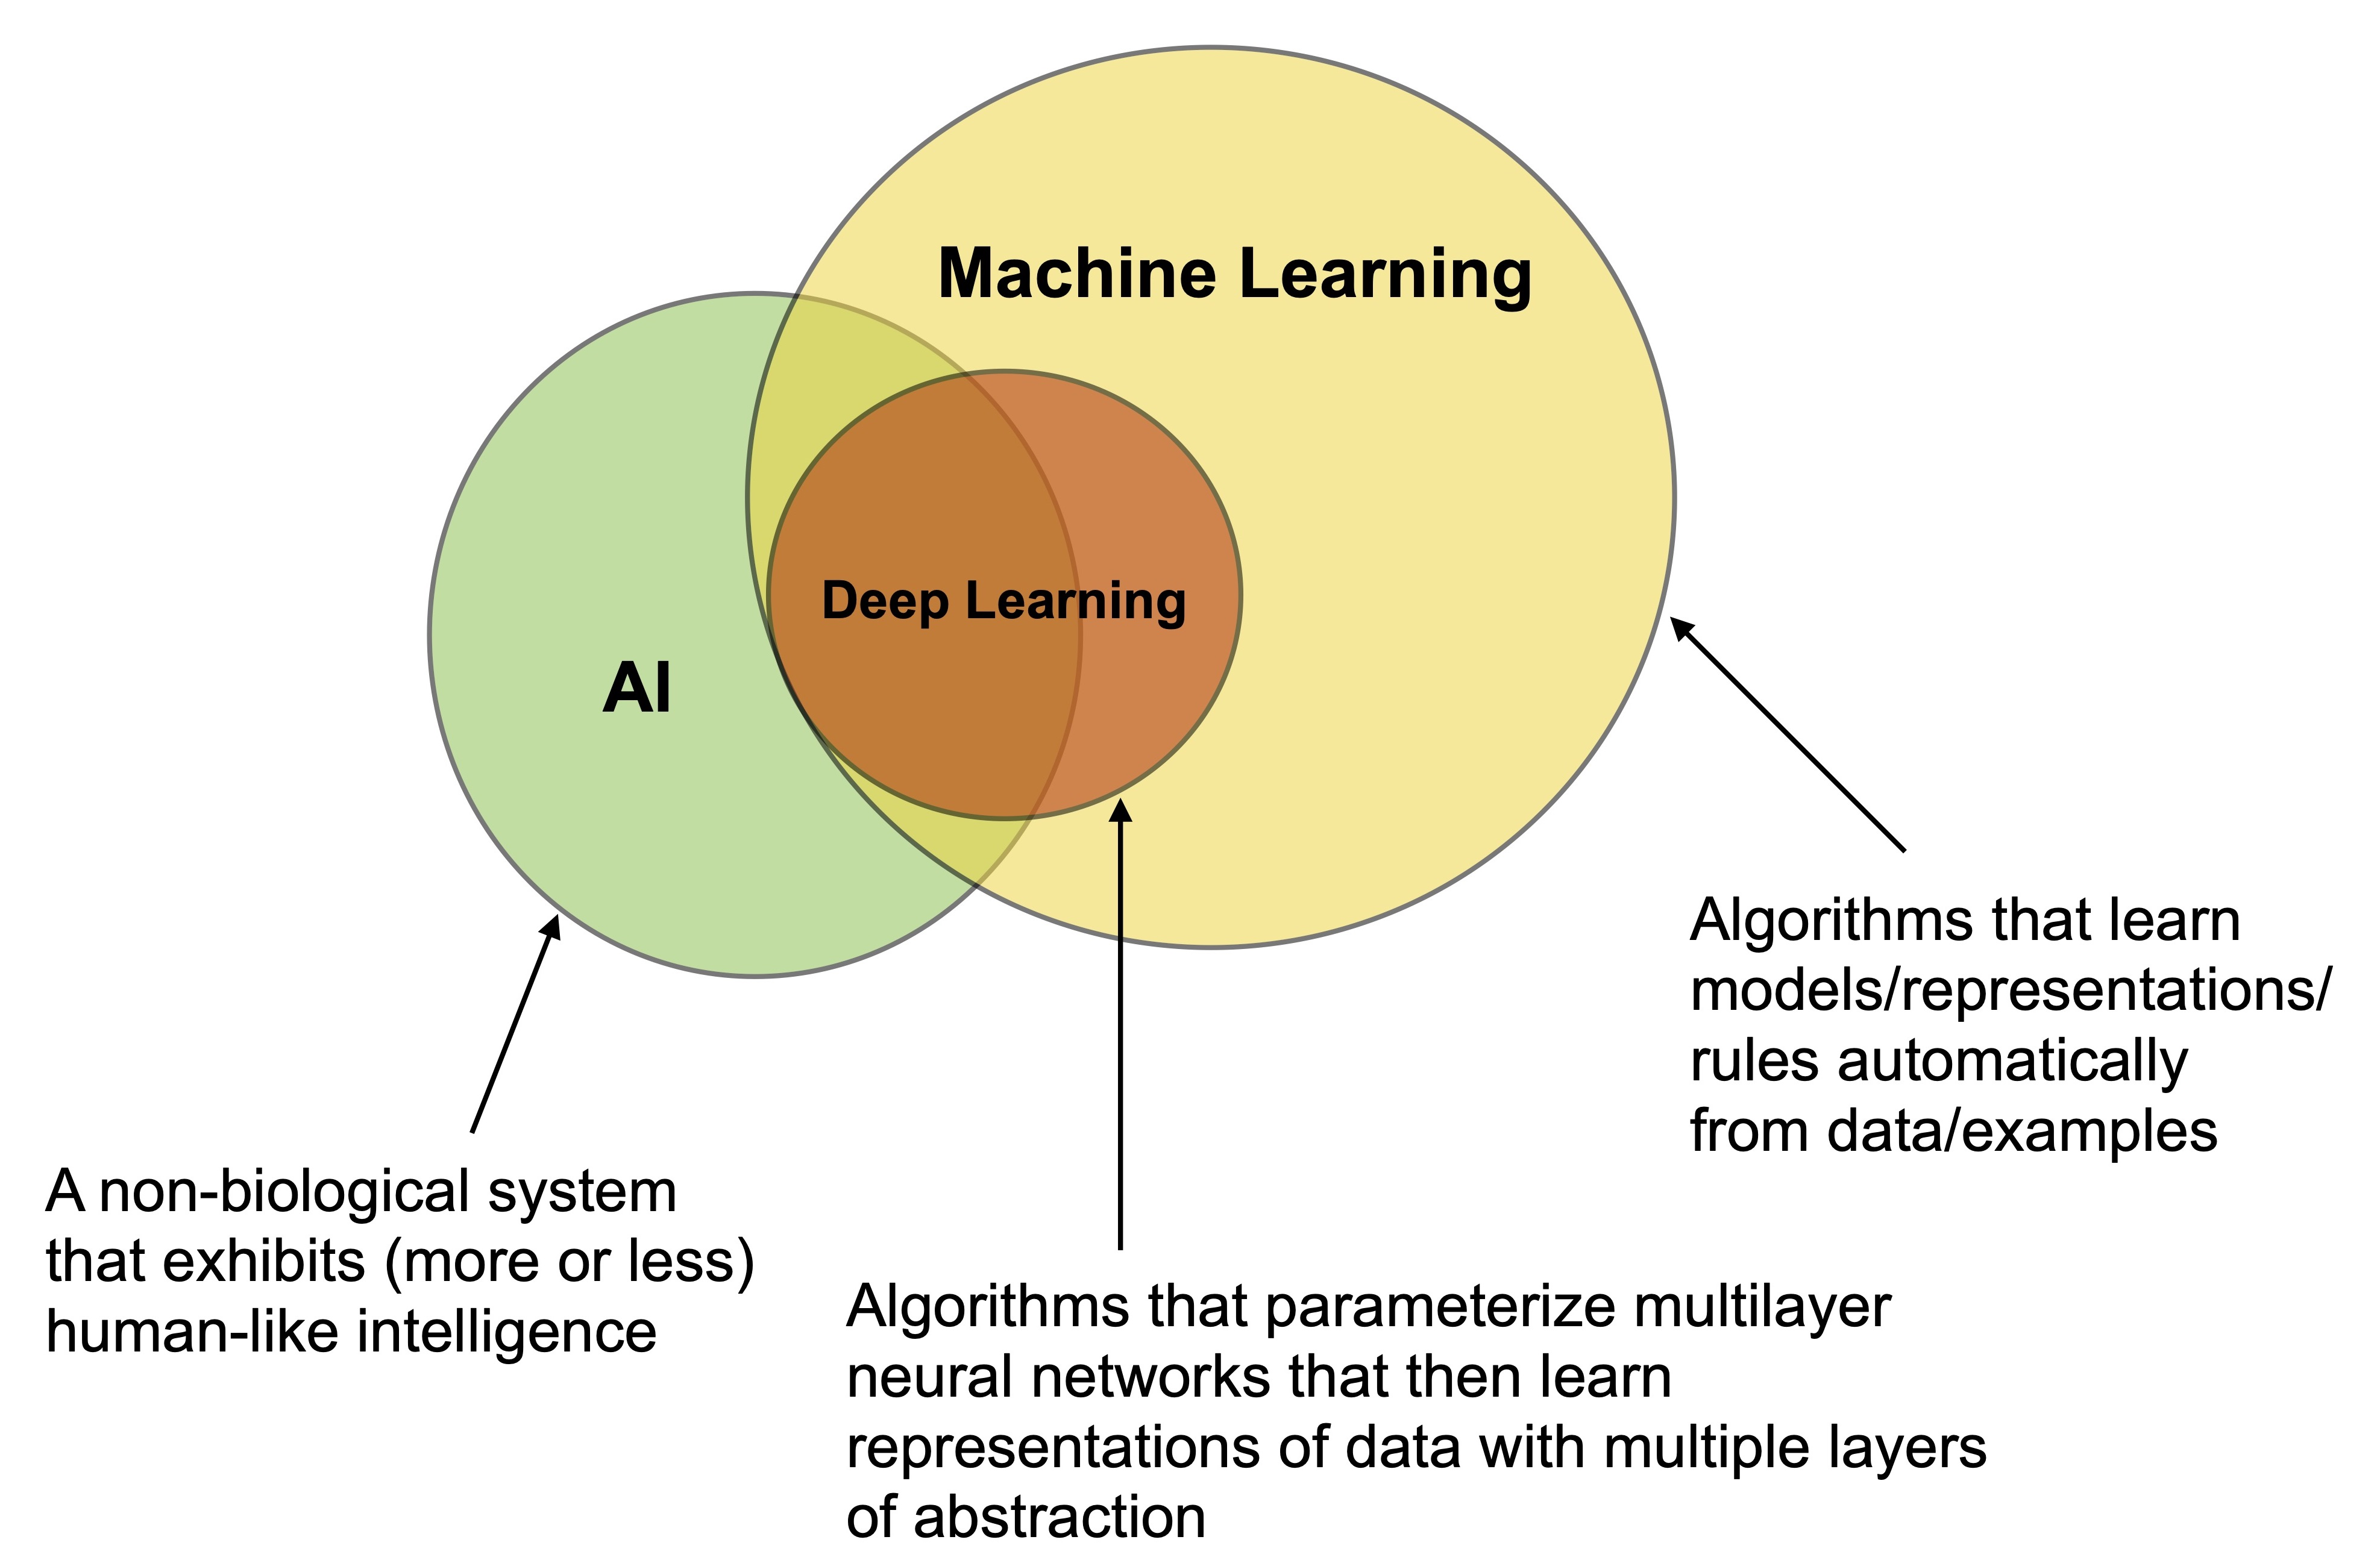
\includegraphics[width=\linewidth]{images/ai_ml_dnn_argue.jpeg}
        \caption[Overview of an alternative structure to the one used in this work for AI, machine learning, and deep learning.]{Overview of an alternative structure for \gls{ai}, machine learning, and deep learning. This structure argues that AI is the pursuit of developing non-biological systems with human-like intelligence and can be achieved with methods that do not use machine learning or deep learning, such as symbolic representations in a shallow architecture. This representation is not de facto and is not used in this work.\\Figure by Sebastian Raschka \cite{raschkaChapterIntroductionMachine2020}}
        \label{fig:ai_ml_dnn_argue}
    \end{figure} 

    \begin{figure}[htb]
        \centering
        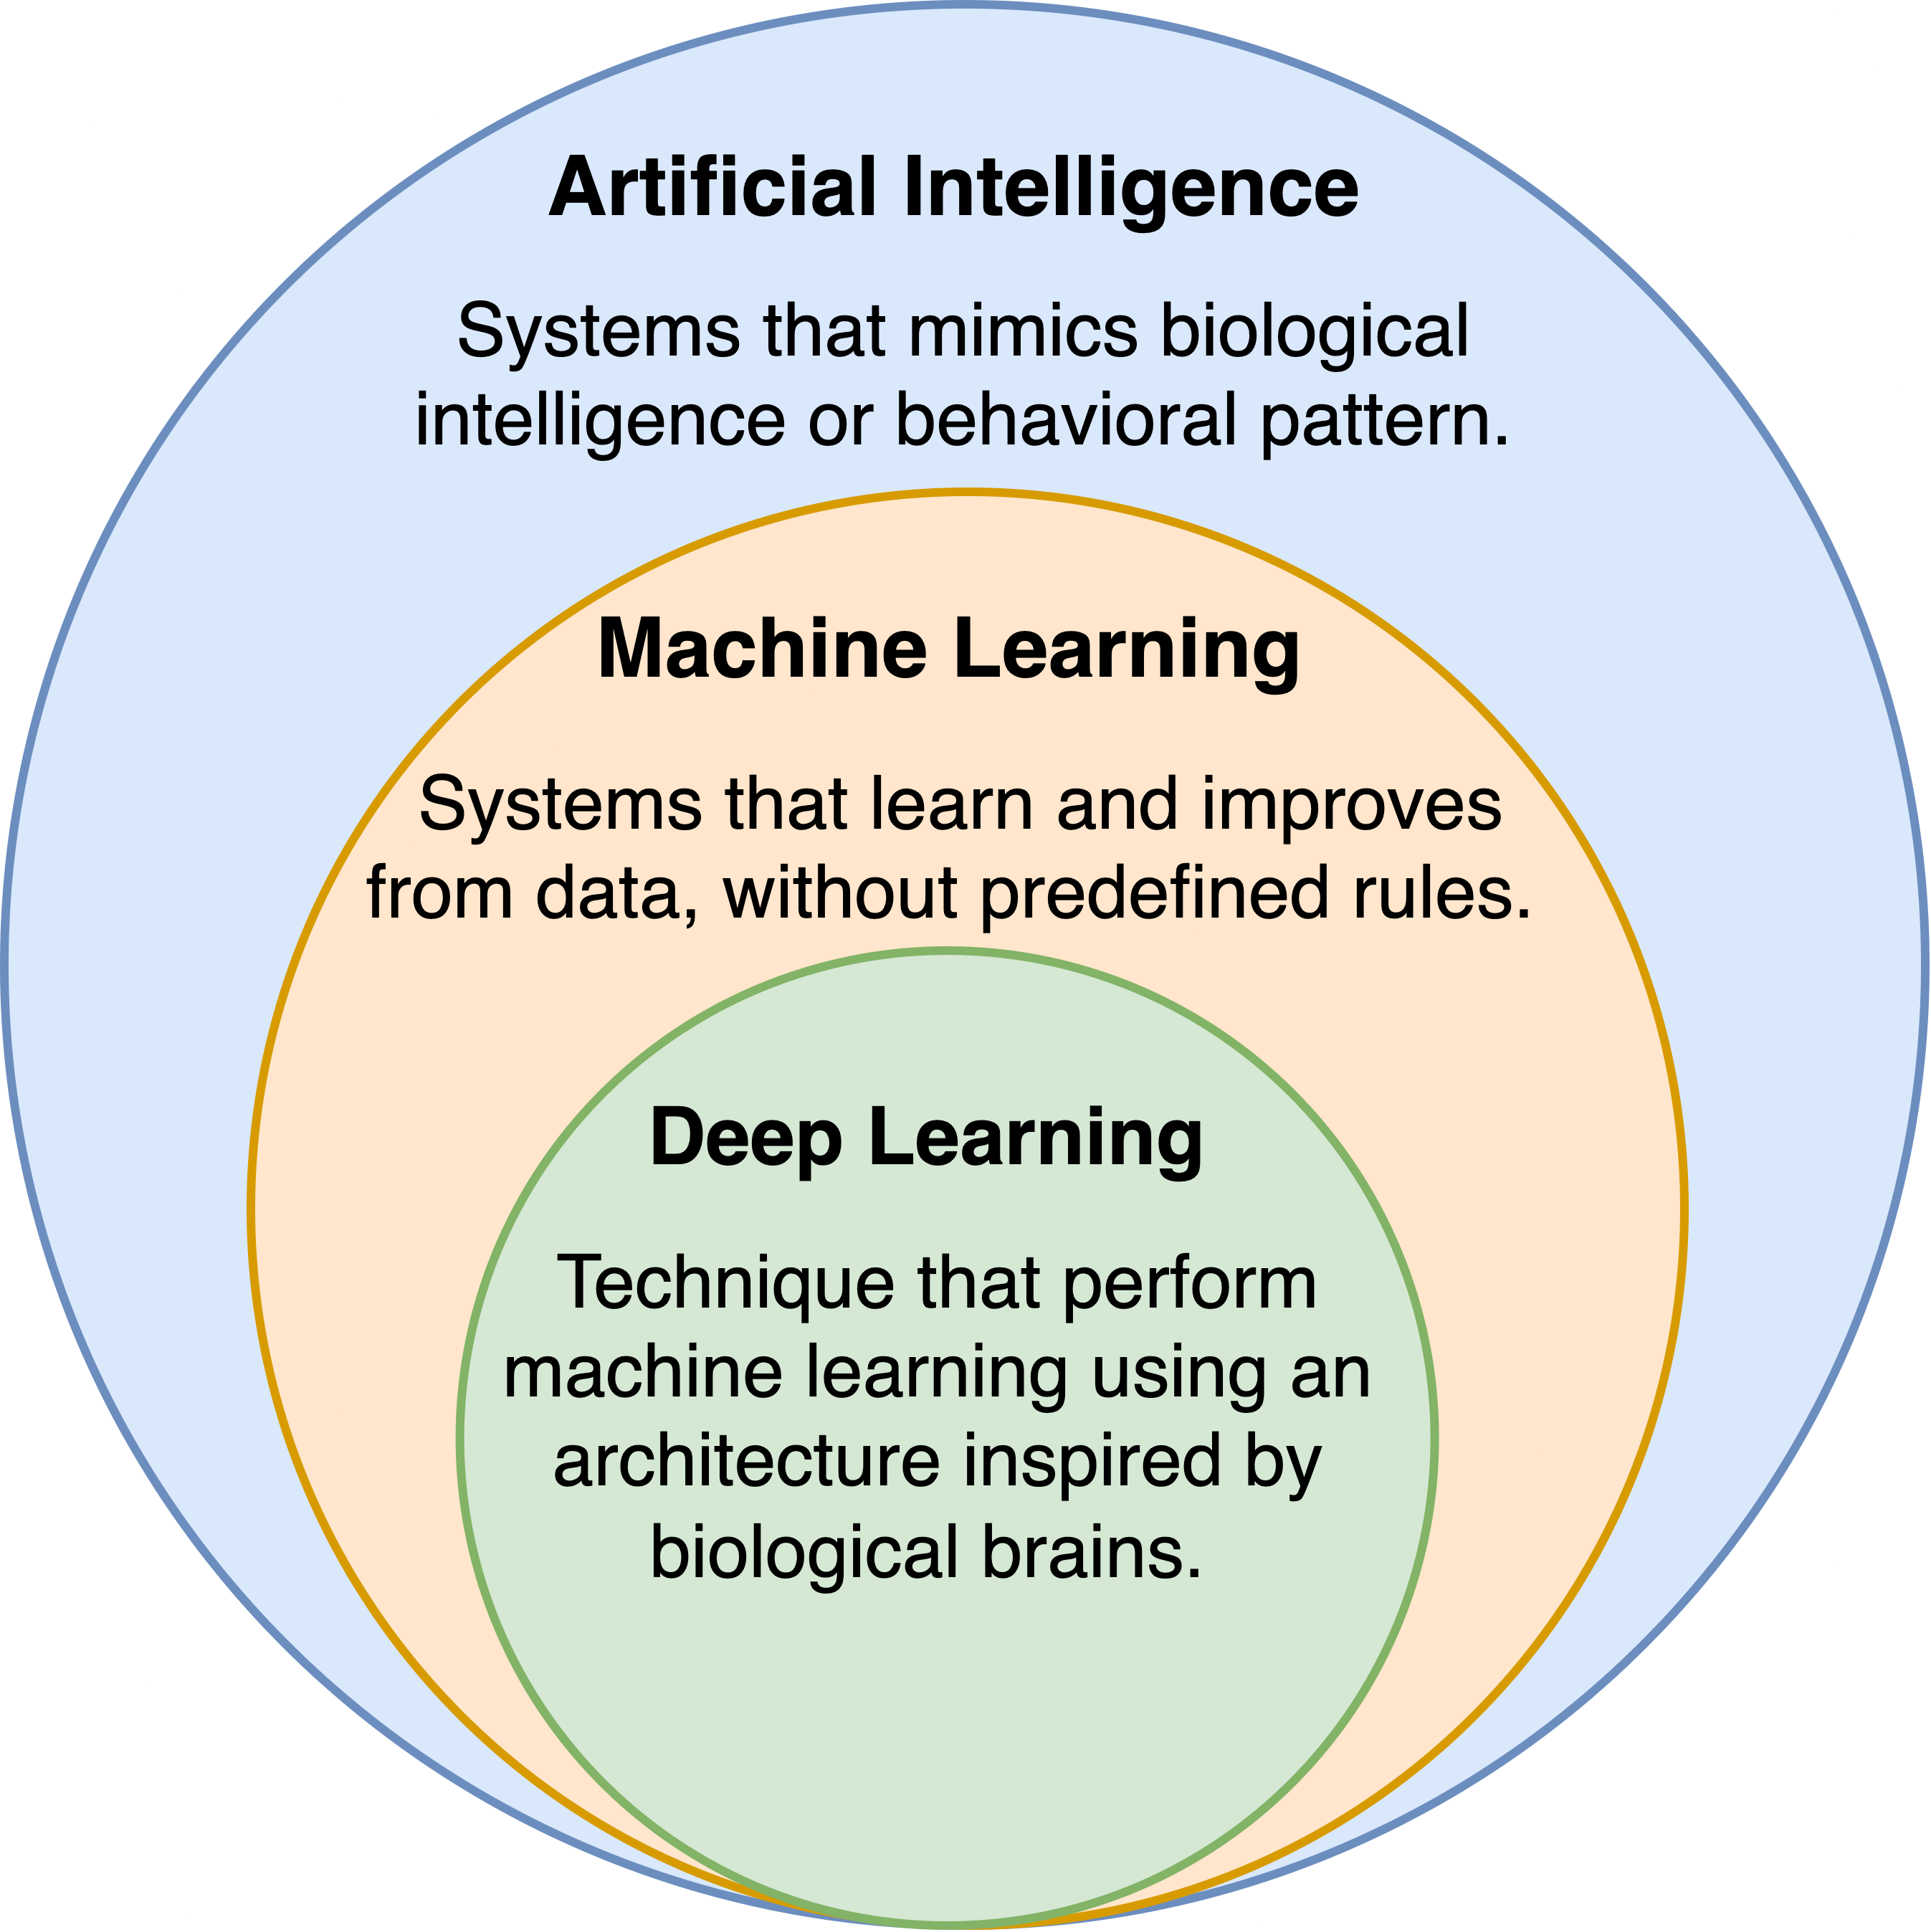
\includegraphics[width=9cm]{images/ai_ml_dnn}
        \caption[Overview of the structure between artificial intelligence, machine learning, and deep learning. This is the structure used in this thesis.]{Overview of the structure between artificial intelligence, machine learning, and deep learning. This is the structure used in this thesis.% Figure by the author.
        }
        \label{fig:ai_ml_dnn}
    \end{figure} 

    Machine learning is often broken down into three sub-areas, which are discussed and explained in this sub-section, explaining how they work, under what circumstances each sub-area can be used to advantage, and the challenges each branch faces are highlighted.

        \subsubsection{Supervised Learning}

        The first category within machine learning is known as supervised learning. This method is conceptually similar to using flashcards for memorization.
        The participant draws a card and reads the question while keeping the answer hidden. Only after the participant answers the question, the correct answer can be revealed. This is, in essence, the same approach used in supervised learning.
        
        
        In supervised learning, a dataset with pre-labeled examples, also known as a fully labeled dataset, is used to train algorithms to predict labeling for unlabeled input data. This is typically accomplished by training on a larger dataset with labels for each input, passing the input through a network, and using the label to inform the algorithm what the input data should be labeled as. In this way, the method learns the relationship between the input and the correct label. The method learns these correlations by adjusting the weights within the network to produce a result that is as close as possible to the true label.
        
        Since the ground truth label is known for each entry in the dataset, the model's output is compared to this ground truth label. The accuracy of the similarity between these two is measured using a loss function. 
        A loss function is a calculation that computes the loss of a single model prediction. The loss is a measure of how far from the ground truth the prediction was and is used to adjust the model to predict better next time. 
        Weights are adjusted using a technique called backpropagation to minimize this loss, and training continues until the weights are appropriately adjusted to achieve a satisfactorily low loss. These weights are then used later when testing real-world inputs, for which ground truth is often unavailable and must be estimated.
        
        Within supervised learning, there are two main subcategories: classification and regression. 
        
        Classification is a method used when the output variable belongs to a category, such as a color or an object, or to indicate the probability that an input belongs to one or more categories. Classification either predicts categorical class labels or classifies data by building a model. A typical classification method can be used to sort emails into spam or not spam or to identify the bird species in an image. Classification models can include methods such as neural networks, \gls{svm}, \gls{knn} \cite{fixDiscriminatoryAnalysisNonparametric1989, coverNearestNeighborPattern1967}, random forest, decision trees, one-vs-rest, and naive Bayes. Section \ref{sec:2_background_theory_deep_learning_and_neural_networks} will go into more detail about neural networks, as this is a central method of machine learning and is relevant to this work, as it is used later in this thesis by the first proposed architecture in Section \ref{sec:3_proposed_architecture}.
        
        The second approach within supervised learning is called regression. This method is used when the output should be a real or continuous value. Regression is used to find the correlation between dependent and independent variables. There are many different models within regression, such as linear regression, logistic regression, and polynomial regression. It is common to use hyperplanes that fit the available data. Hyperplanes are defined as a subspace of a vector space and have one less dimension than the vector space they are inside. These planes, therefore, are used to make a cut in the feature space in order to separate data samples.
        Regression is often used to make forecasts based on past data, e.g., estimating real estate prices for an area or salary growth.


        \subsubsection{Unsupervised Learning}

        Unsupervised learning is a technique that uses raw data from a given dataset to identify patterns and relationships in unlabeled data, facilitating the grouping of each item into appropriate clusters. The essence of this approach is that it can autonomously analyze and group data without requiring human intervention to pre-label the data. Therefore, it is well suited for use in data analysis, image recognition, and image segmentation.

        
        
        The main grouping models used in unsupervised learning are clustering, association, and dimension reduction. Clustering aims to divide raw data into groups or clusters based on similar characteristics. An example of a cluster split is shown in Figure \ref{fig:knn}, demonstrated by the \gls{knn} method. Association rules, on the other hand, are a rule-based approach that attempts to uncover relationships between variables in a dataset. These associations can, for example, be used in recommendation models, where companies can identify correlations between customers who purchase different items and use this knowledge to suggest similar products to new customers.

        \begin{figure}[htb]
         \centerline{
             \begin{subfigure}[b]{0.37\textwidth}
                 \centering
                 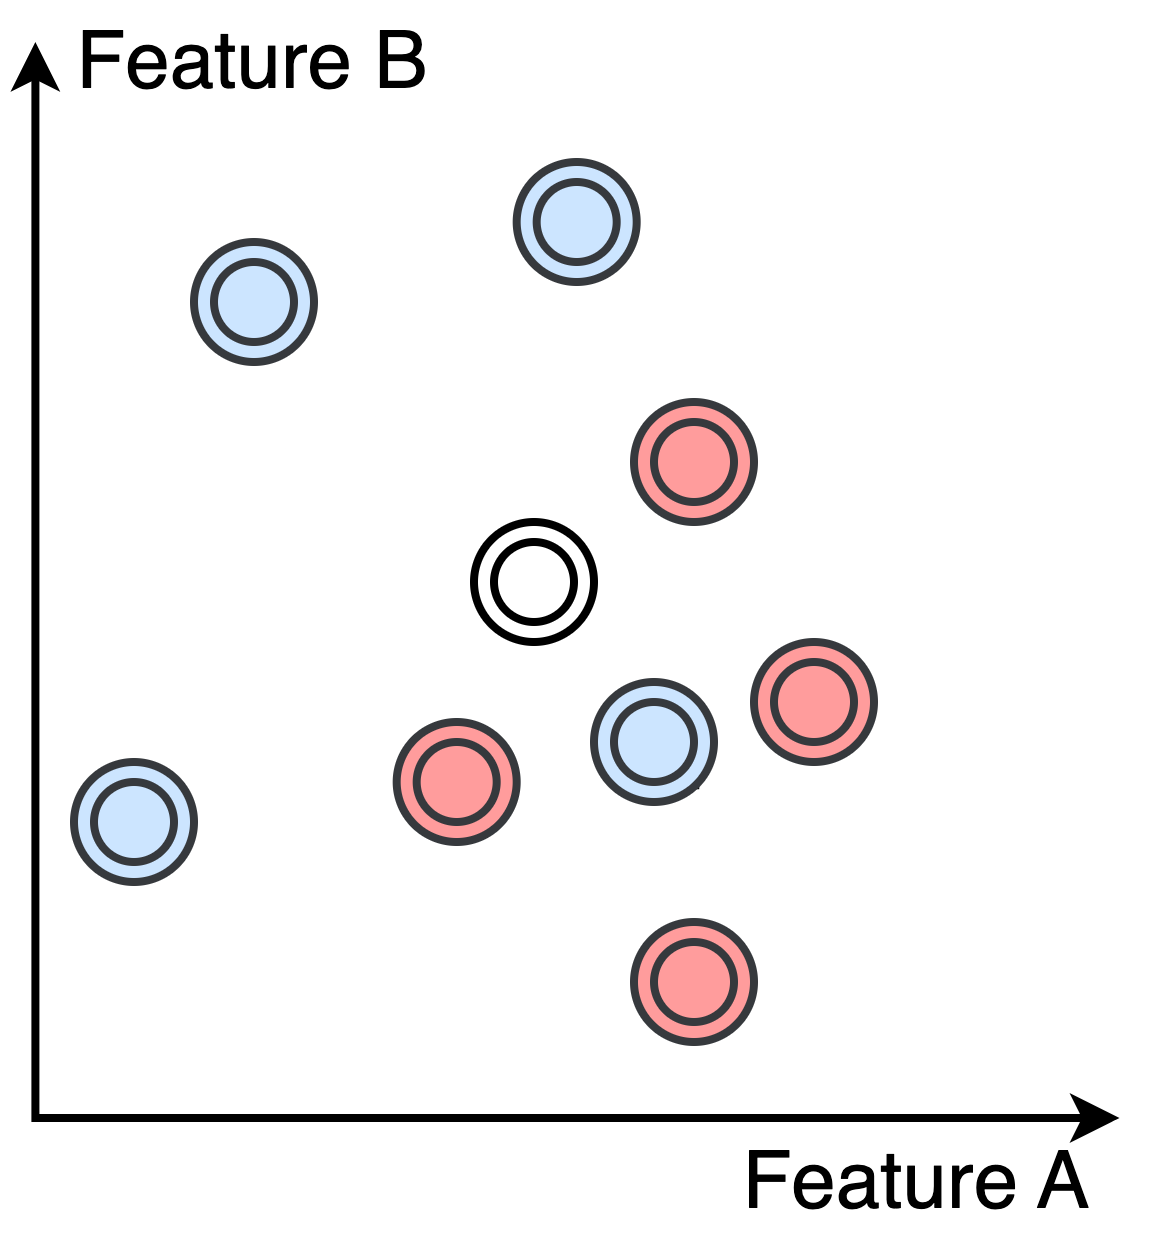
\includegraphics[width=\textwidth]{images/knn_1}
                 \caption{Samples are distributed in a feature space. The colors represent class, and the white is a new sample. A new sample will be classified based on neighboring samples.}
                 
             \end{subfigure}
             \hspace{0.015\textwidth}
             \begin{subfigure}[b]{0.37\textwidth}
                 \centering
                 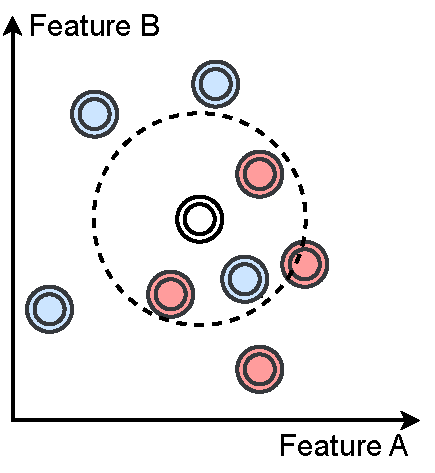
\includegraphics[width=\textwidth]{images/knn_2}
                 \caption{The new sample checks the nearest neighboring samples. In a circumference, noted with a dotted circle, the 4 closest neighboring samples are found.}
                
             \end{subfigure}
             \hspace{0.015\textwidth}
             \begin{subfigure}[b]{0.37\textwidth}
                 \centering
                 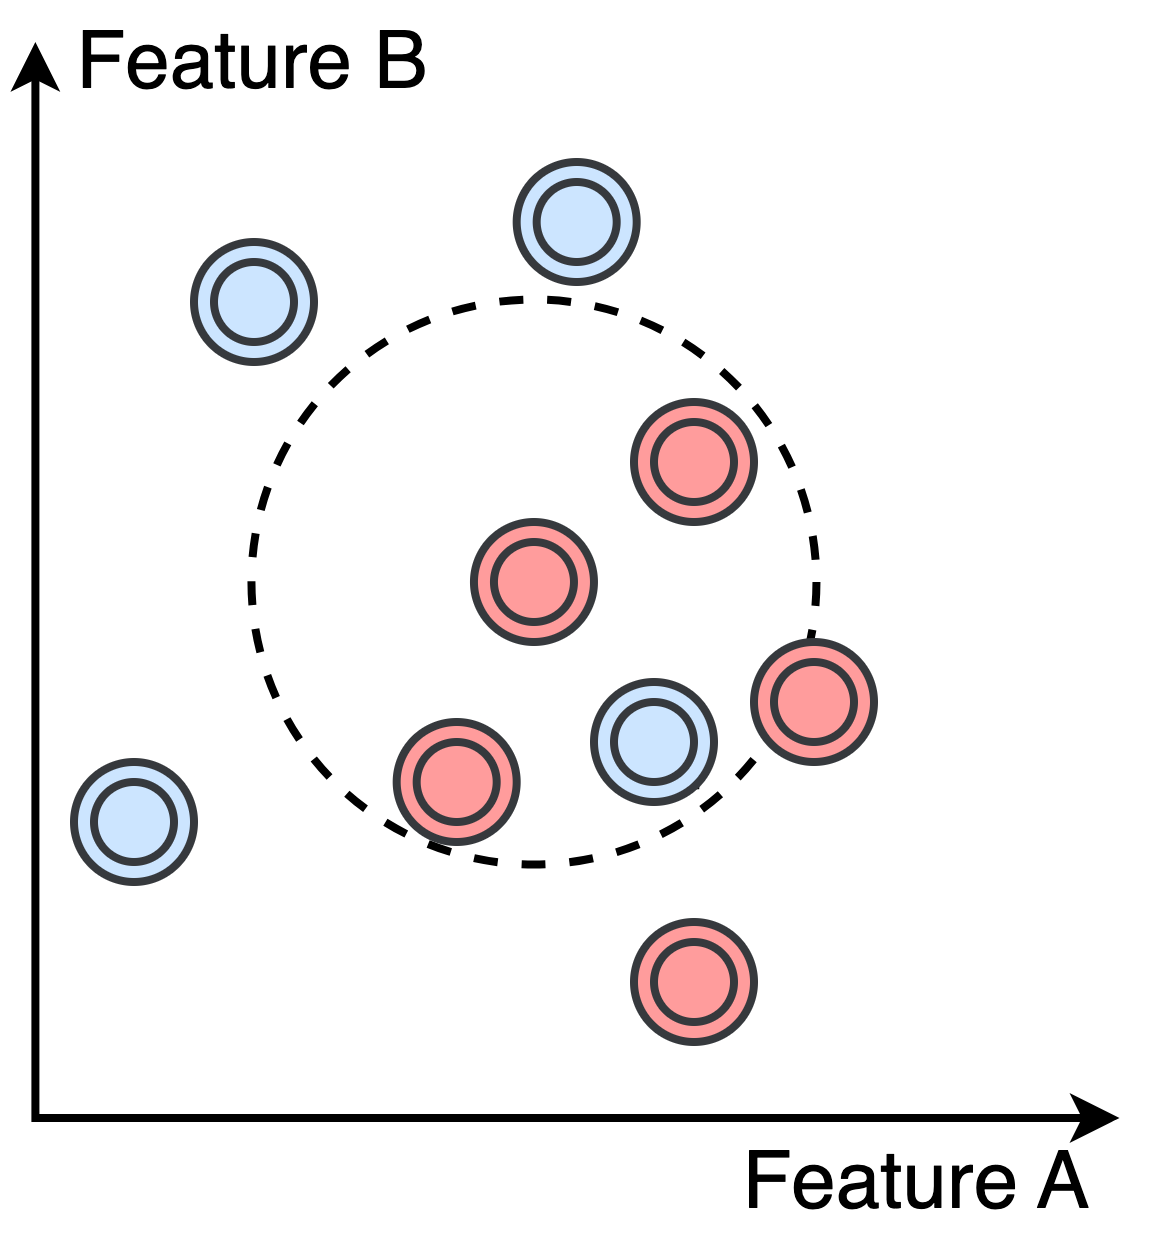
\includegraphics[width=\textwidth]{images/knn_3}
                 \caption{The classes of the 4 closest samples are counted, and the majority class is chosen. Of the 4 samples, one is blue, and three are red. The new sample is therefore classified as red.} 
             \end{subfigure}
             }
            \caption[Figure showing k-Nearest Neighbors clustering.]{Example of how the clustering algorithm k-Nearest Neighbors computes the class of a new sample. 
            %Figure by the author.
            }
            \label{fig:knn}
        \end{figure}
        
        Dimensionality reduction is a technique for reducing the number of dimensions in a dataset. 
        Although many machine learning methods benefit from additional data, this is not always the case \cite{belkinReconcilingModernMachinelearning2019, nakkiranDeepDoubleDescent2021}. Data samples can often contain insignificant variables or noise, making model training ineffective and making the dataset in practice smaller regarding useful information. This technique can be used to create a dataset containing more distinct features and also visualize and analyze data. When reducing the dimensions of a dataset, the goal is to reduce the number of learnable parameters while maintaining the integrity of the data being processed. Well-known methods for dimension reduction are \gls{pca} and \gls{svd}. More recently, good results have been obtained with deep neural network-derived autoencoders \cite{sakuradaAnomalyDetectionUsing2014}. Autoencoders can compress data fed to them and produce a representation or encoding that retains much of the underlying data, but the dimensions are significantly reduced.
        To retrieve this data after encoding, a decoder is required to reconstruct the data. Figure \ref{fig:auto_encoder} depicts an autoencoder with an encoder and decoder.

        \begin{figure}[htb]
            \centering
            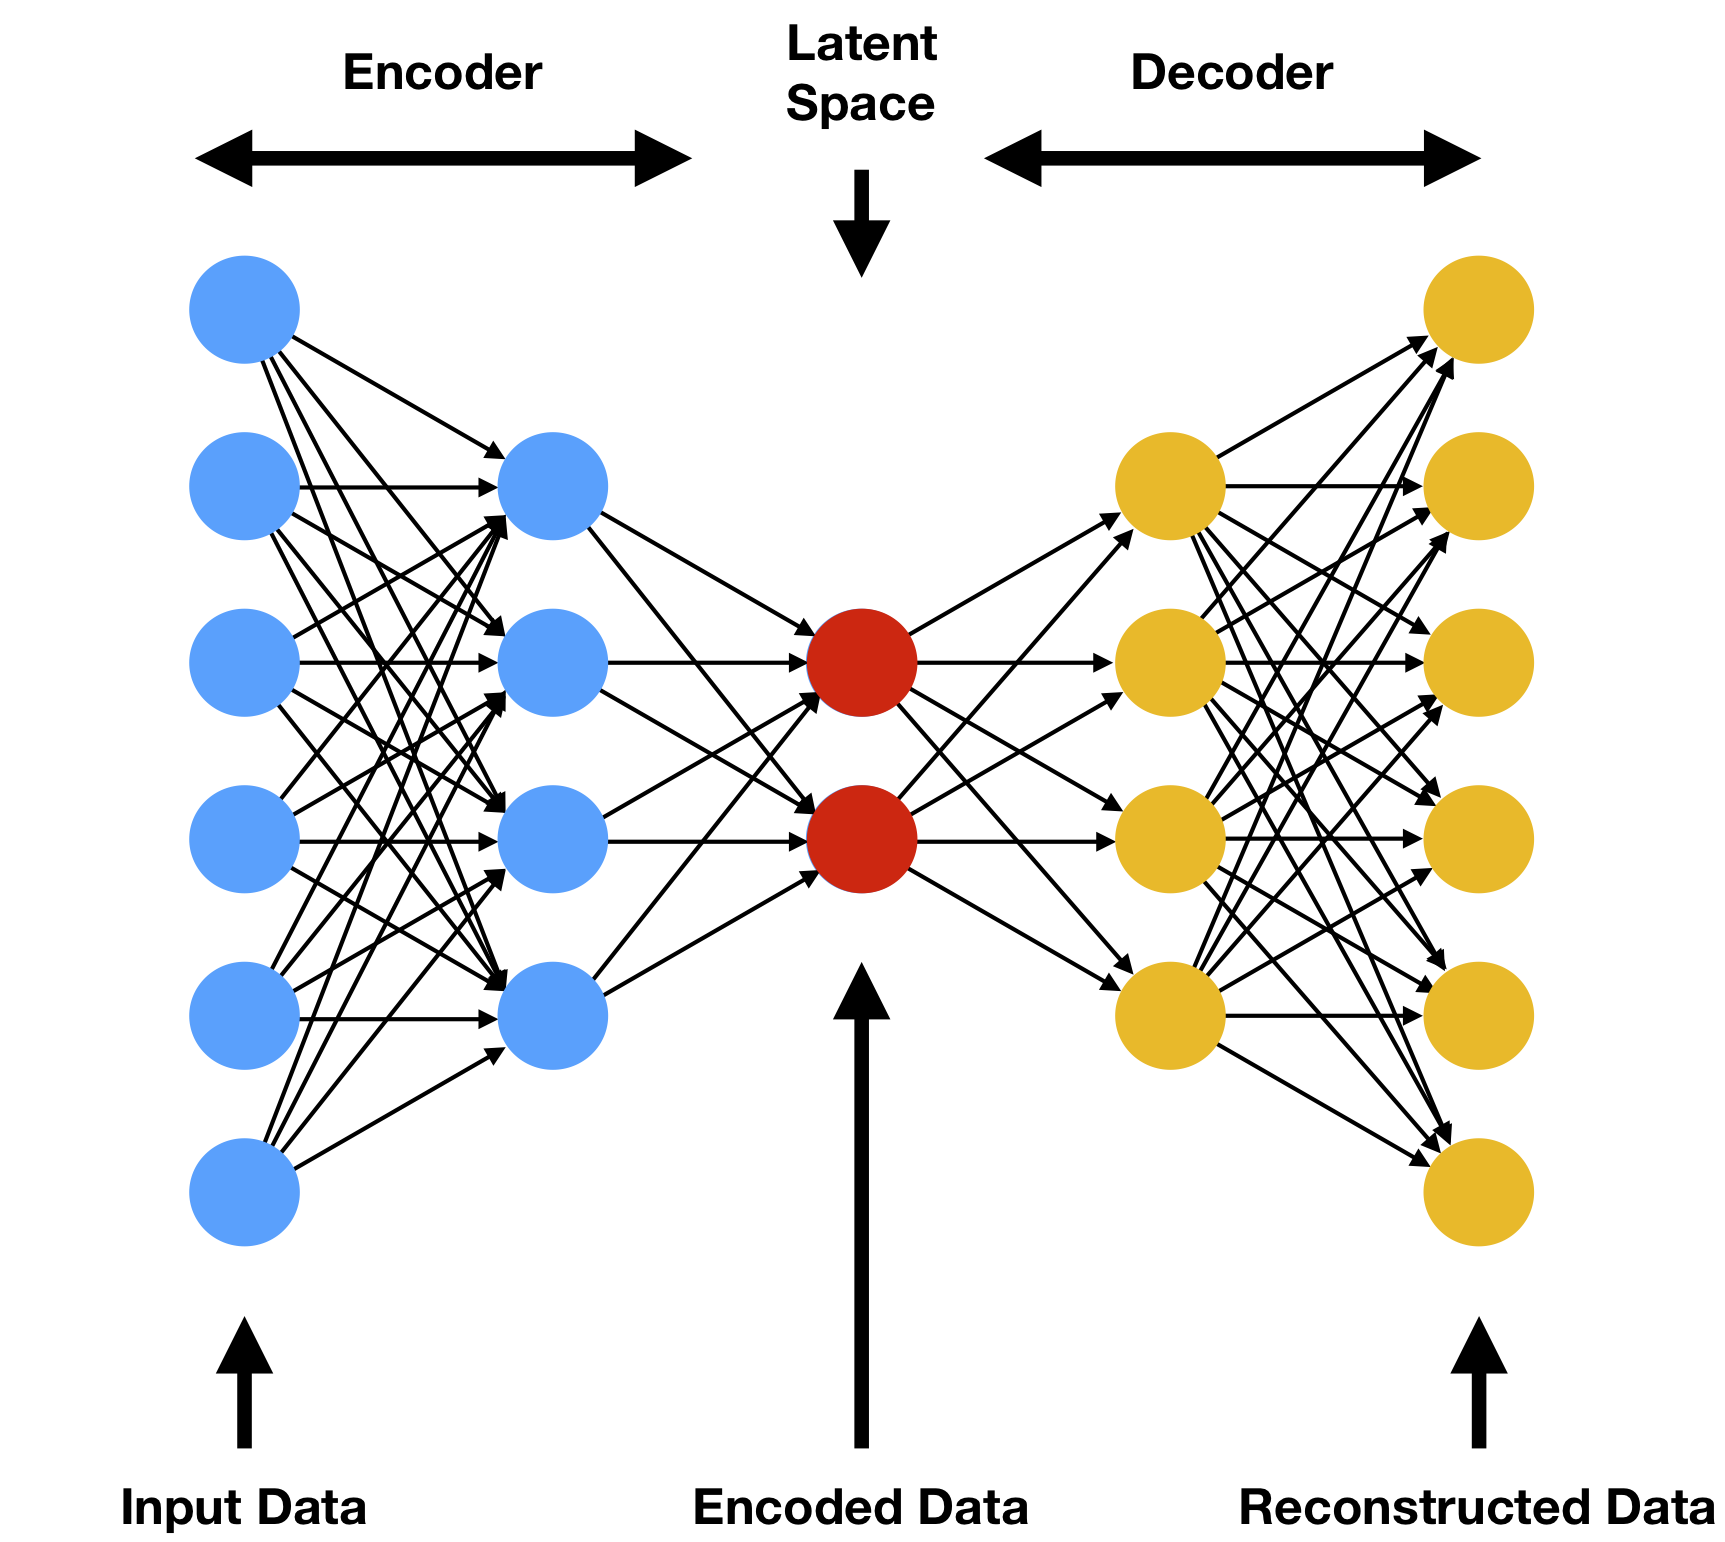
\includegraphics[width=\textwidth]{images/auto_encoder}
            \caption[Figure of an autoencoder.]{A diagram of an autoencoder consisting of an encoder and a decoder network. The encoder network maps the input image into a low-dimensional representation, while the decoder network reconstructs the original image from the low-dimensional representation. By minimizing the reconstruction error between input and output, the autoencoder can learn a compressed representation of the input data.\\Figure inspired by Steven Flores \cite{floresVariationalAutoencodersAre2019}.}
            \label{fig:auto_encoder}
        \end{figure} 
        
        Unsupervised learning has proven useful in computer vision, where it can aid in object recognition, detection, and segmentation, such as in medical datasets. By allowing correlations to be identified and grouped into clusters based on features or traits, unsupervised machine learning can also be used for anomaly detection, where it can flag atypical data. This method is also often used in recommendation engines, such as those found in online stores, streaming services, or social media.


        \subsubsection{Semi-Supervised Learning and Hybrids}

        % https://en.wikipedia.org/wiki/Semi-Supervised_Learning#Semi-supervised_learning
        % https://en.wikipedia.org/wiki/Active_learning_(machine_learning)
        % https://ai.stanford.edu/blog/weak-supervision/
        % https://medium.com/geekculture/weak-supervision-and-active-learning-352fe8dc7df8
        % https://snorkel.ai/weak-supervision/
        % https://www.youtube.com/watch?v=SS9fvo8mR9Y
        % https://www.youtube.com/watch?v=-cc2RYF37zE

        Supervised learning is often more accurate than unsupervised learning as it can learn from the knowledge provided by humans in the form of labeled data. This approach can also avoid computational complexity since the model does not need to train on irrelevant features for the specific task. However, the downside of supervised learning is that it requires significant human effort beforehand labeling the dataset, which can be time-consuming and costly, particularly when domain experts are required.

        A hybrid solution that aims to leverage the best of both supervised and unsupervised learning is known as semi-supervised learning. This approach can be beneficial when there is too much data to label, either because the dataset is large or the cost of labeling is high. Semi-supervised learning typically assumes that data points close together in feature space share labels or have an underlying correlation factor in a lower dimension (manifold hypothesis/assumption). Methods using semi-supervised learning often achieve higher accuracy than those using only supervised or unsupervised approaches separately. This is because they do not need to discard data that is not labeled and can be trained using a researcher's \textit{a priori} knowledge of the dataset or possible solution \cite{reddySemisupervisedLearningBrief2018, berthelotMixMatchHolisticApproach2019}.
        
        Other approaches, such as active learning and weak supervision, can also often be used when a fully labeled dataset is unavailable for training. Active learning is a process in which a model can select input data about which it is unsure and ask a human or other expert for the correct answer. For example, such methods can label large data sets with services such as Amazon Mechanical Turk \cite{AmazonMechanicalTurk}. Samples are selected using a model that attempts to ask for samples believed to have the highest value for further classification. This can be achieved by first asking an expert for a sample from random samples and fitting the model to obtain a decision boundary that separates the classes. After that, the model can iteratively identify examples of high importance since they are near or at this decision boundary. These are the most uncertain examples, making them valuable for the model to identify. Then the model asks the expert for samples near the boundary. The boundary is adjusted again, and the process is repeated until the model fits the data and satisfactorily separates the samples.
        
        Weak supervision is a method that can be applied in situations where it is preferable to have a large number of sufficiently accurate examples rather than a smaller number that are completely correct \cite{hoffmannKnowledgeBasedWeakSupervision2011}. This approach is often implemented by defining some rules or using a knowledge base in advance, which helps the model estimate the probability that an example belongs to a certain category. Weak supervision is often used in conjunction with transfer learning, which involves transferring knowledge from one area to another \cite{wangSimVLMSimpleVisual2022}. Transfer learning has shown promising results because generalizable knowledge of data can often be transferred, eliminating the need to learn from scratch on a new dataset. Transfer learning can be combined with other methods, e.g., supervised learning \cite{zhuangComprehensiveSurveyTransfer2021}.
    
    \subsection{Deep Learning and Neural Networks} \label{sec:2_background_theory_deep_learning_and_neural_networks}
    Neural networks, also known as \glspl{ann}, are a machine learning method inspired by how the biological brain processes information and learns. Essentially, \glspl{ann} approach the goal of extracting information and constructing knowledge by forming a network of artificial neurons that can process input data. These artificial neurons, called perceptrons, are the building blocks of neural networks and are likewise inspired by biological neurons. In this representation, the inputs to the artificial neuron are synapses on the dendrites, the axon hillock inspires the activation function, and the output from the artificial neuron is the biological axon.
    
    The artificial neurons process data by weighting the input data and a predetermined bias before passing it through an activation function, such as a sigmoid or \gls{relu} \cite{dubeyActivationFunctionsDeep2022} that produces the neuron's output. When the output of the activation function exceeds a certain threshold, the neuron is activated and sends data to the next layer. No further data is sent if the output does not exceed the threshold.

    \begin{comment}
    % Remove this
    This processing step of a perceptron can be viewed as a linear regression, as in shown formula ?. However, unlike linear regression, perceptrons in \glspl{ann} are connected in a network, so changes in weights cascade to the next level of perceptrons. A single-layered neural network can therefore be seen as a logistic regression function.
    \end{comment}
    
   \glspl{ann}, often called multi-layer perceptron (MLP), are the cornerstone of deep learning, which refers to \glspl{ann} with more than three layers. The smallest deep network, therefore, has an input layer, two hidden layers in the middle, and an output layer. These middle processing layers are called the hidden layer because it is hidden from the outside, which the input and output layers are not. An example of such a network with two hidden layers is shown in Figure \ref{fig:deep_network} to see. 


    \begin{figure}[htb]
        \centering
        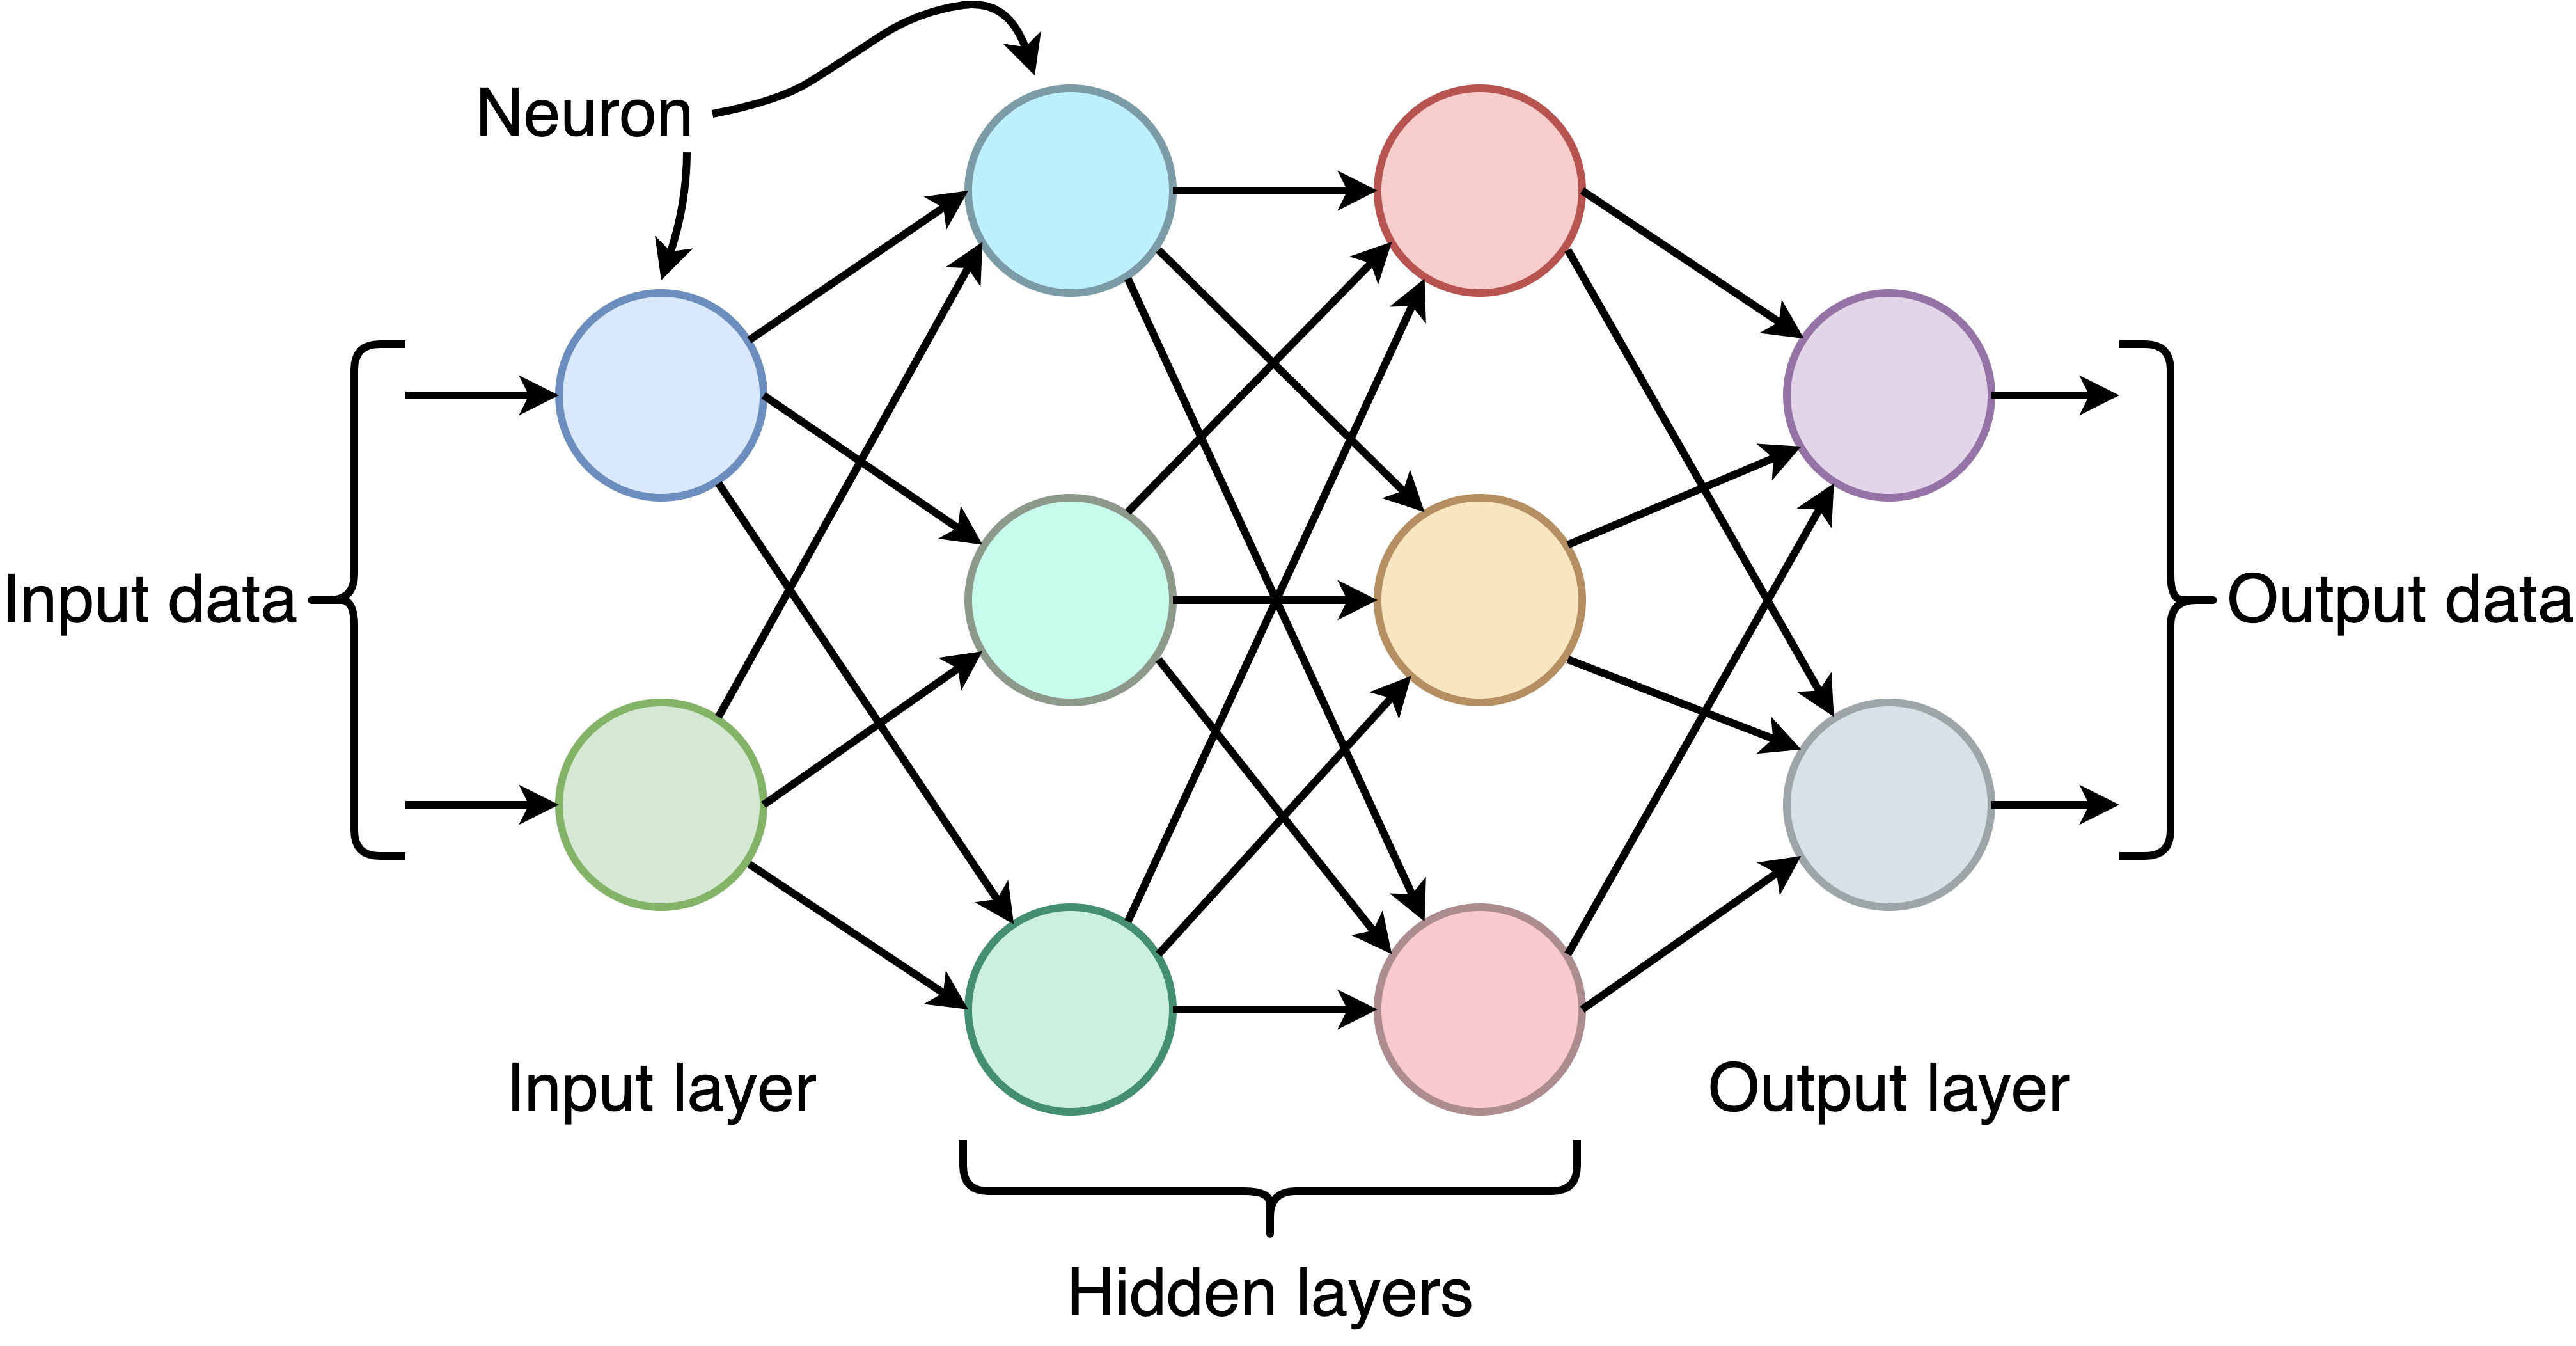
\includegraphics[width=\linewidth]{images/deep_neural_network}
        \caption[Figure of a fully connected deep artificial.]{A fully connected deep artificial neural network with two hidden layers and two input and output neurons.} %Figure by the author.}
        \label{fig:deep_network}
    \end{figure}

   
    
    Most \glspl{ann} are feedforward, meaning that data is entered on one side, passed through the network, and produces a result on the other end. These networks are often trained using backpropagation, where the network output is compared to the ground truth, and the difference between the estimated result and the ground truth is used to adjust the network weights to minimize this difference. The backpropagation technique is also inspired by biological backpropagation, which occurs when a neuron generates an action potential that sends a voltage spike back to the dendrites. Other methods are proposed instead of feedforward combined with backpropagation, such as the proposed forward-forward algorithm by Geoffrey Hinton \cite{hintonForwardForwardAlgorithmPreliminary2022}.


    Deep neural networks have achieved remarkable achievements, mainly due to their ability to learn from structured and unstructured data. This allows them to learn and generalize knowledge given sufficient amounts and high-quality data \cite{willeminkPreparingMedicalImaging2020}. Before computing power allowed deep networks, hand-made feature extractors were commonly used, using human-predefined features such as texture, shape, and color for object recognition tasks. However, when deep learning was first used in the \gls{imagenet} competition \cite{russakovskyImageNetLargeScale2015}, which is a competition identifying objects from the ImageNet dataset \cite{dengImageNetLargeScaleHierarchical2009}, it achieved great results as shown in Figure \ref{fig:imagenet_results_graph}. This figure shows the methods and their classification error for each year the competition was arranged. It is clear that deep learning made significant strides in 2012 with AlexNet, which was proposed by Krizhevsky et al. \cite{krizhevskyImageNetClassificationDeep2017}. These methods have improved significantly since then, largely thanks to improved methods and hardware. In 2015, deep learning even surpassed the human ability to classify images in ImageNet with the ResNet model proposed by He et al. \cite{heDeepResidualLearning2015, heDelvingDeepRectifiers2015}.
    
    \begin{figure}[htb]
        \centering
        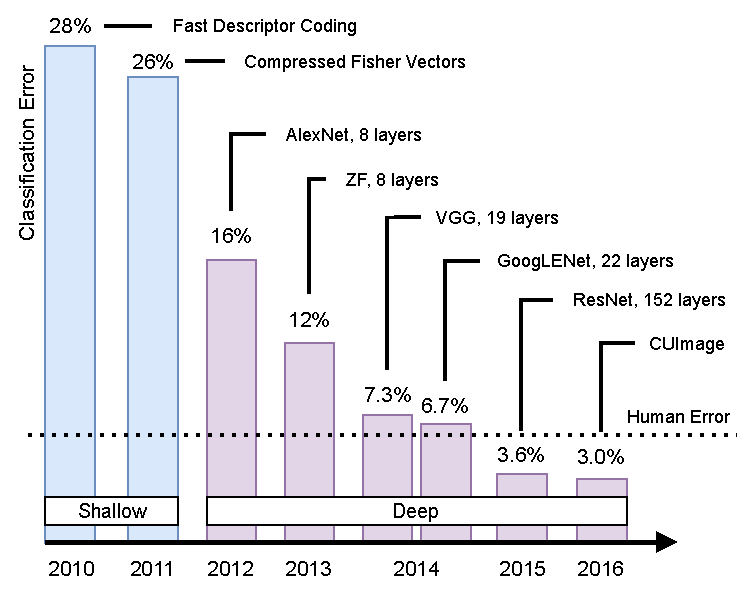
\includegraphics[width=\linewidth]{images/imagenet_results_graph}
        \caption[ImageNet competition winners from 2010 to 2016.]{Overview of the ImageNet competition winners from 2010 to 2016. The figure shows how deep networks have significantly improved the networks' ability to guess the right label for the images in the ImageNet dataset. In 2015, the deep network ResNet \cite{heDeepResidualLearning2015} surpassed the average human ability to label these images correctly. \\
        Figure inspired by Gordon Cooper \cite{cooperSoftwareFrameworkRequirements2017}.}
        \label{fig:imagenet_results_graph}
    \end{figure}


    
    \subsection{Convolutional Neural Networks}

    % Intro to CNNs
    Inspired by biology alongside regular neural networks, the computer vision method called \glspl{cnn} is designed to mimic how the brain's visual cortex processes visual information. \gls{cnn} builds on the idea and technique of neural networks and adds at least one convolutional layer. A convolutional layer allows information about neighboring entities to be obtained from the previous layer. The method has proven particularly effective in computer vision to process and analyze images and video because it can gather context from nearby areas where the convolution is centered. This can help the method extract contextual and semantic relationships that would otherwise have been lost. Both of the proposed methods presented in this thesis use a \gls{cnn}, namely a VGG-16 model \cite{simonyanVeryDeepConvolutional2015}, to classify images and extract image features. Therefore, understanding how \glspl{cnn} are constructed and their advantages and uses are relevant.

    % Intro to convolution layers
    The convolution layer works by scanning small filters across the input image, computing dot products between the filter and the image pixels at each location, and creating a feature map. A convolution layer can be considered a flashlight beam aimed at an image. The beam of light allows the viewer can see areas of the image that are in the perimeter of the area where the center of the beam is directed. As the beam of light moves across the image, the viewer can comprehend more of what is in the image. An illustration of a convolution is shown in Figure \ref{fig:convolutuon}.

    \begin{figure}[htb]
        \centering
        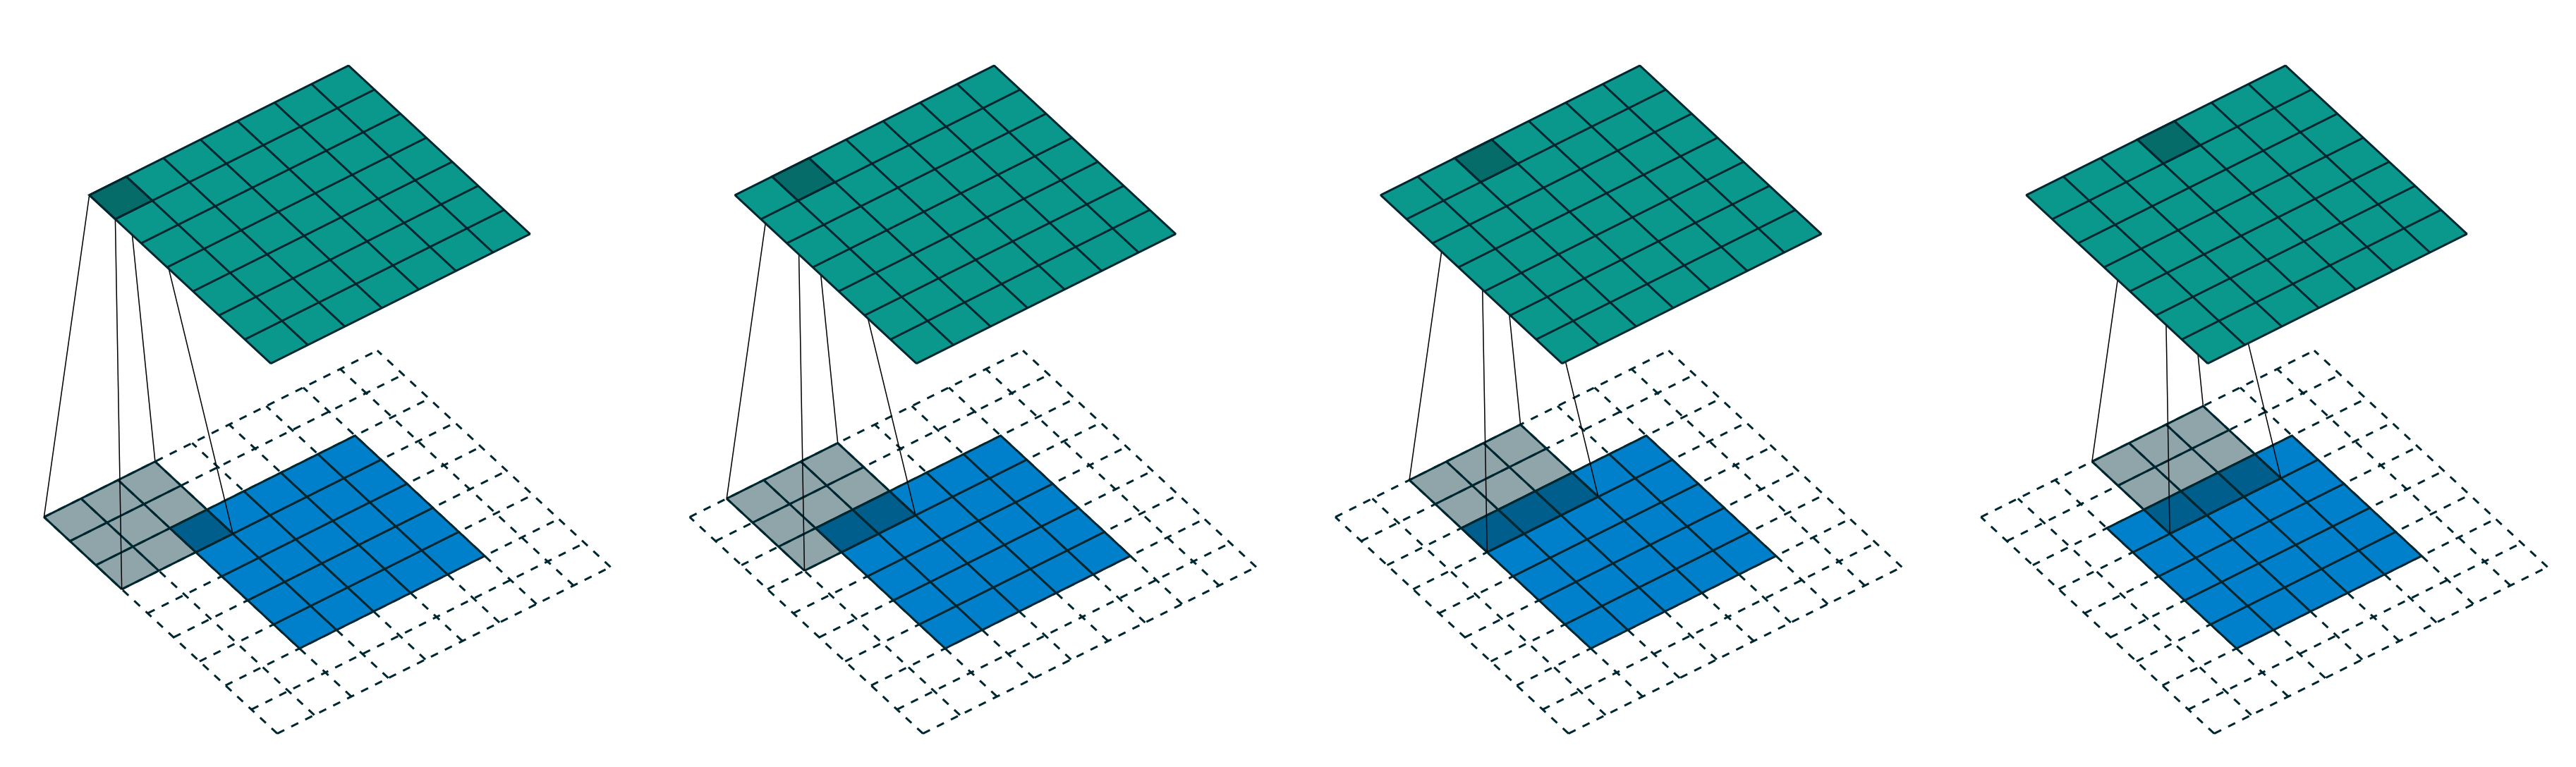
\includegraphics[width=\linewidth]{images/convolution.png}
        \caption[Illustration of a convolution.]{An illustration of a convolution where a $3 \times 3$ kernel is convolved with a $5 \times 5$ input matrix. The convolution illustrated has full padding and a one-step stride.\\
        Figure by Vincent Dumoulin and Francesco Visin \cite{dumoulinGuideConvolutionArithmetic2018}.}
        \label{fig:convolutuon}
    \end{figure}


    % Short history and advantage.
    The first \gls{cnn} that trained with backpropagation was first proposed by LeCun et al. in 1989 \cite{lecunHandwrittenDigitRecognition1989} and has since had a huge importance in making machines interpret images and videos. A major advantage of using a convolutional layer is that it can compress information while preserving information and the context around the retrieved information. A very common \gls{cnn} architecture is shown in Figure \ref{fig:vgg_cnn}. Also seen in the figure is that a typical \gls{cnn} has a fully connected neural network. A \gls{cnn} often uses fully connected layers, unlike a normal neural network, because of the condensation of information with surrounding information, allowing for a network that can take advantage of using many parameters without overfitting.  

    \begin{figure}[htb]
        \centerline{
        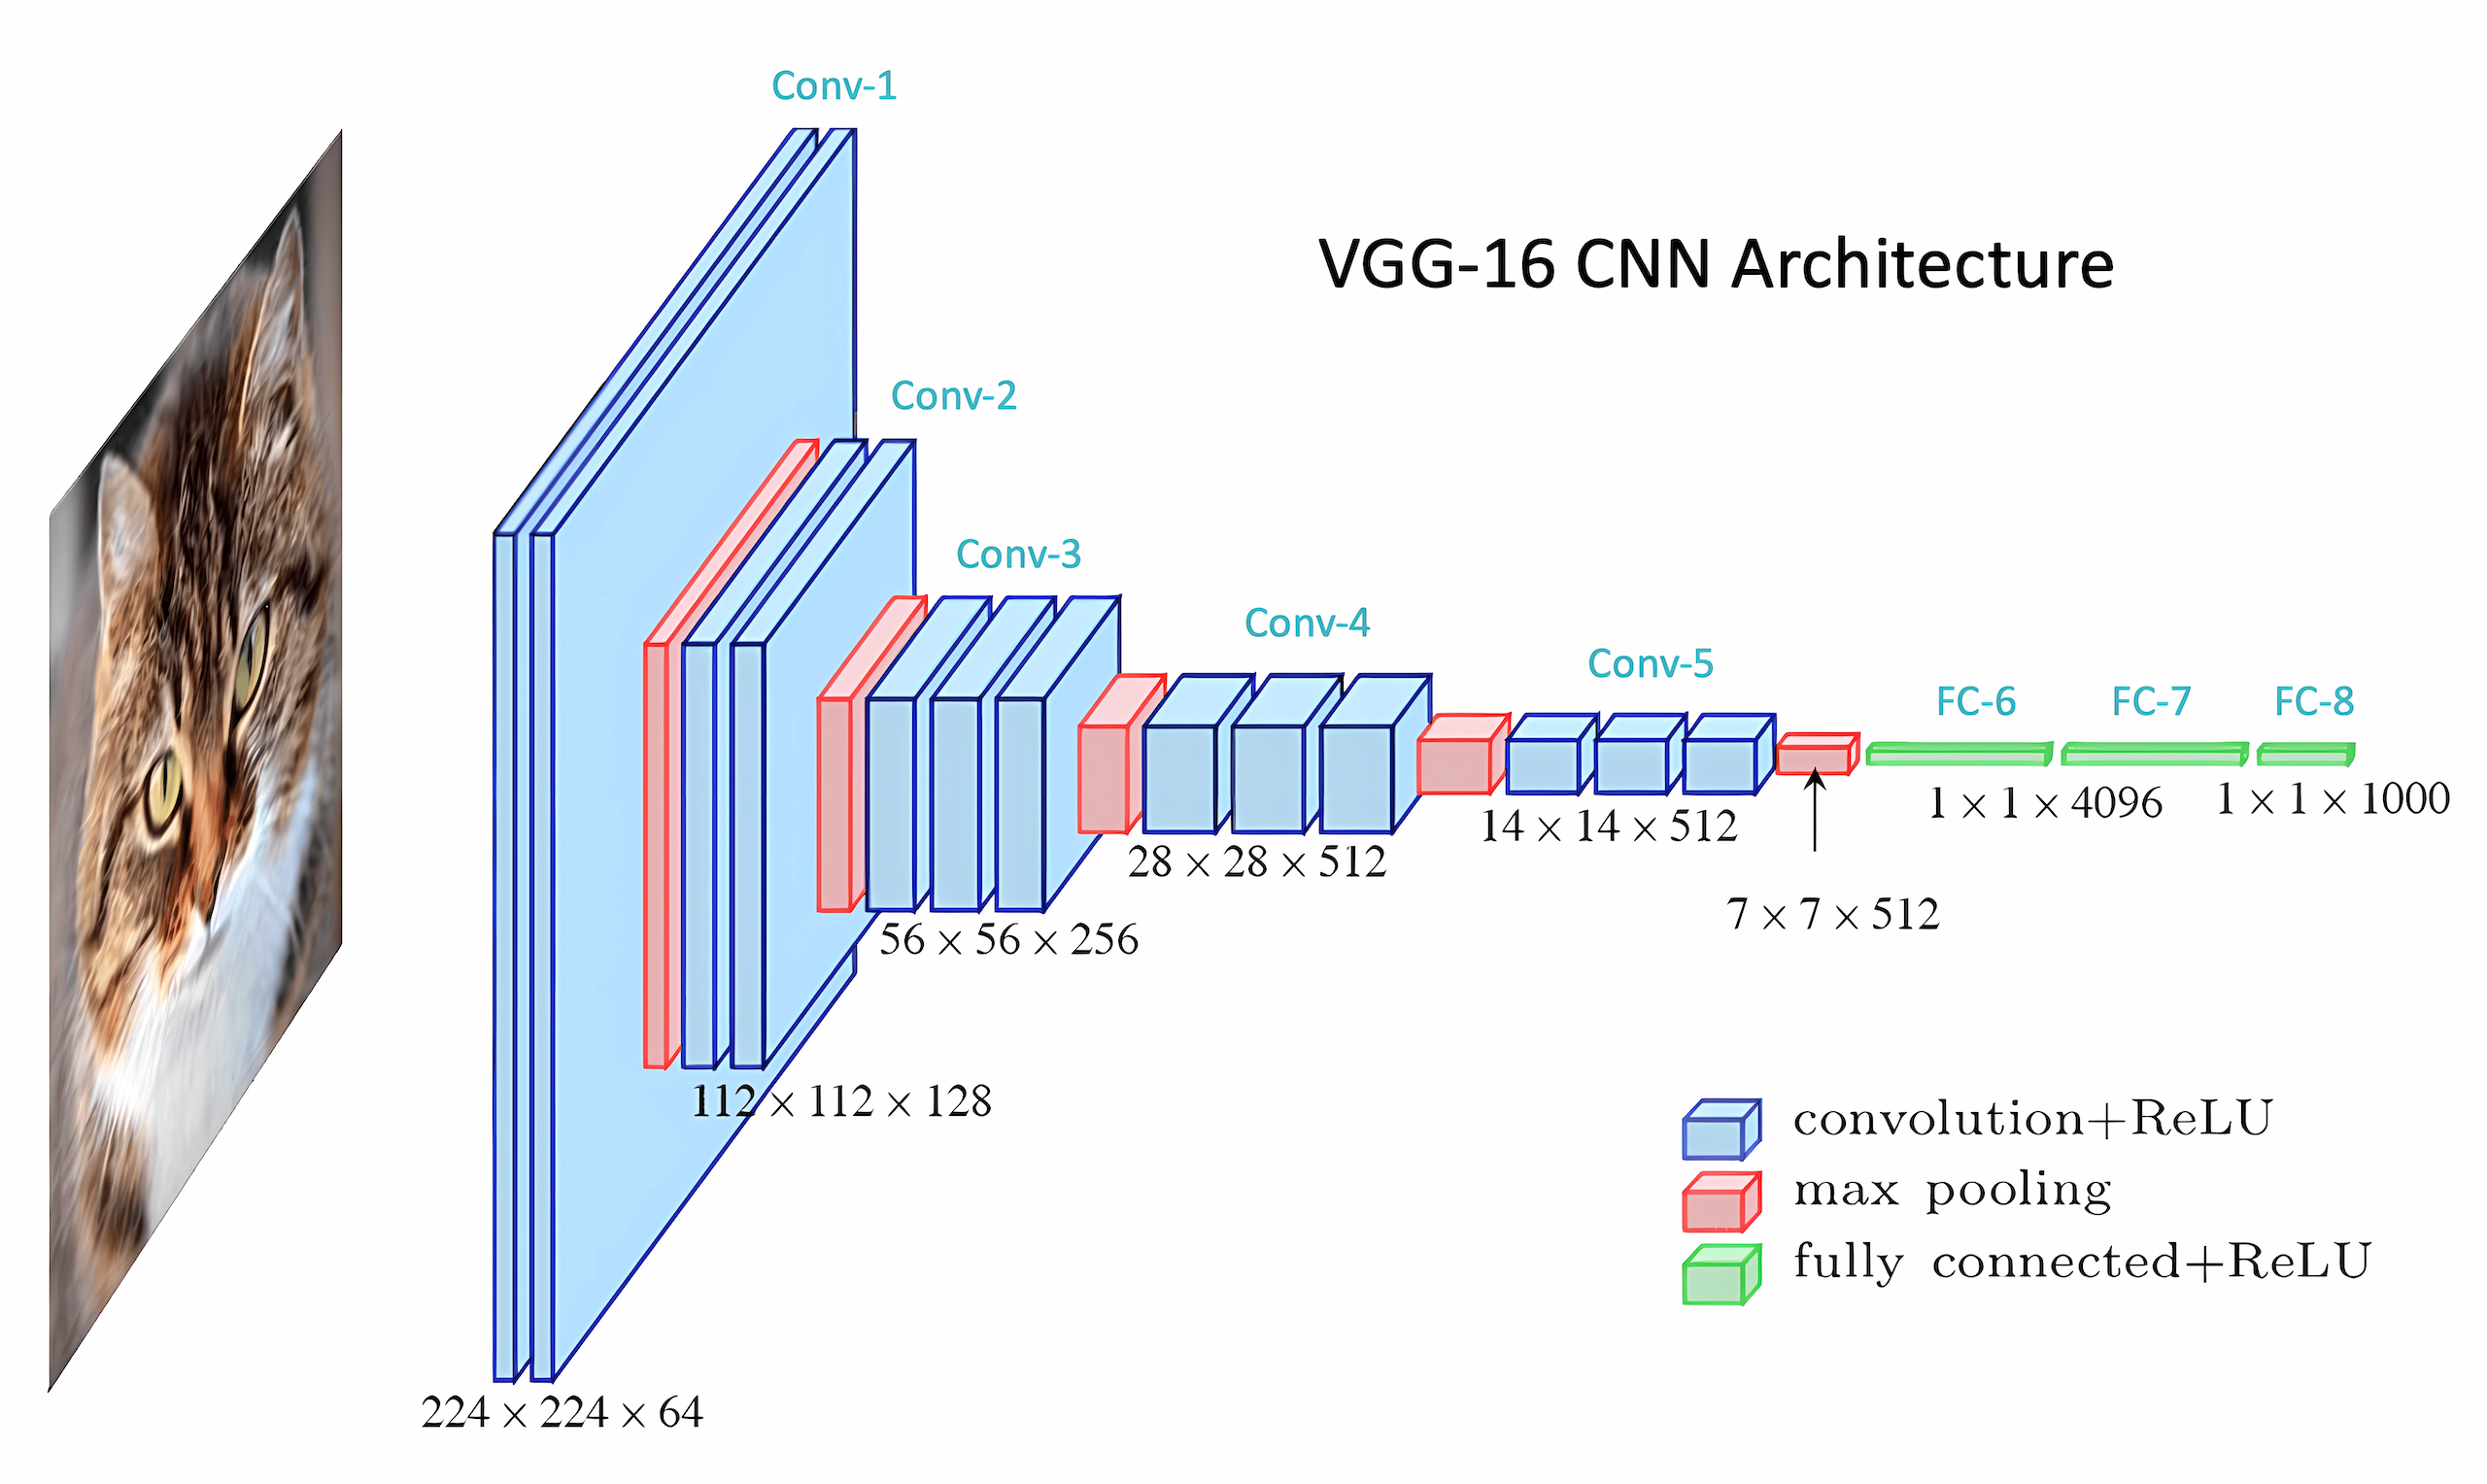
\includegraphics[width=1.1\linewidth]{images/vgg_cnn.png}}
        \caption[Example of a CNN architecture, illustrated by the VGG-16.]{Example of a typical CNN architecture, here illustrated by the VGG-16 model proposed by Simonyan and Zisserman \cite{simonyanVeryDeepConvolutional2015}. As seen in this figure, the first part of the network convolves the input image and extracts feature maps. These feature maps are then fed into a fully connected artificial network that classifies the image in a given class.\\
        Figure by Satya Mallick \cite{UnderstandingConvolutionalNeural2023}.}
        \label{fig:vgg_cnn}
    \end{figure}
    
    The convolution layers can be applied to an input image as a series of filters, producing a series of feature maps that emphasize different aspects of the image. These filters have weights that are learned and adjusted during training and are able to recognize different types of patterns of increasing complexity and abstraction from the input image. The training process is similar to regular neural networks. It typically updates weights using backpropagation to minimize the loss function and improve the accuracy of the network on the training set. The first layers, closest to the input image, generally recognize low-level features such as edges, lines, corners, texture, and color. As the convolutional layers process the input information, more complex features can be detected that build an abstraction on the information extracted from earlier layers. Convolution layers farther from the image can recognize more high-level features such as shapes, objects, and scenes. Overall, the convolutional layers allow the features of the input image to be analyzed hierarchically, with the early layers capturing low-level features and the later layers capturing high-level features.
    
    % More in-depth architecture with pooling layers.
    \glspl{cnn} are typically designed with multiple layers, similar to deep neural networks, and the last layers are typically fully connected. The fully connected layers take the output of the convolution layers, a set of feature maps, and convert them into a single vector of class scores that represent the probability that the input image belongs to each possible class. The main function of pooling layers in \glspl{cnn} is to reduce the spatial dimensions of the feature maps generated by convolutional layers while preserving the most salient features of the input image. Pooling layers operate on small regions (e.g., 2x2 or 3x3) of the feature maps generated by the previous convolution layers and reduce their size by applying a pooling function, such as max pooling or average pooling, on each region. Max pooling selects the maximum value within each region as the representative value, while average pooling calculates the mean of the region. These operations effectively downsample the feature maps and help reduce the network's sensitivity to small spatial translations and variations in the input. Pooling layers can be inserted after one or more convolutional layers in a \gls{cnn}. Their hyperparameters, like the size of the pooling area and the stride (i.e., the amount of movement of the pooling window), can be tuned to control the amount of downsampling and the size of the resulting feature maps.
    
    Additionally, pooling layers can prevent network overfitting by reducing the number of parameters and the computation time required for training. The role of pooling layers in \glspl{cnn} is not limited to downsampling. However, they can also help to capture translation invariance, i.e., the property that the learned features are invariant to small translations in the input. The translation invariance is achieved because the max or average operation selects the most prominent feature in a given region, regardless of its exact position. This property allows the network to collect more general relationships in the input data, providing a more general understanding of the network. The overall benefits of pooling layers lie in reducing the spatial dimensions of feature maps while preserving their salient features, resulting in more efficient and robust image analysis.
    
    % Summary
    In essence, the different layers of a \gls{cnn} work together to extract and classify features in images and videos. This makes \glspl{cnn} particularly effective for tasks such as image classification, object detection, and segmentation, where detecting and locating different features of an image is critical for accurate performance. \glspl{cnn} have proven highly effective in image classification tasks, outperforming other types of neural networks and traditional machine learning algorithms. They have been used in various applications, including object recognition, facial recognition, and medical image analysis. With the development of larger and more complex networks and the availability of powerful hardware and software, \glspl{cnn} remains an active area of research and development in machine learning.


\section{Image Captioning}

    The methods proposed in this thesis use techniques to extract information from input images and present a text output. The method to make a model give a textual description to an image is often called image captioning.
    Image captioning is a field of research where the objective is to generate textual descriptions using natural language from the content of an image. This process uses computer vision and \gls{nlp} to gather information from images and give a text that describes or analyzes the image's content. Image captioning is, therefore, a multimodal method that has excelled with the advancements in computer vision, helped considerably by \glspl{cnn} and language models. The motivation for developing this field of research is that its advancements can be utilized in many applications. Image captioning can contribute to improving accessibility for the visually impaired, enhancing search and retrieval systems, assisting in indexing images and video, and making models that can use the combined information in both language and vision to gather information. 

    Image annotation methods typically include modern deep learning techniques, using \glspl{cnn} to extract image features and \glspl{rnn} \cite{rumelhartLearningRepresentationsBackpropagating1986}, typically \glspl{lstm} \cite{hochreiterLongShorttermMemory1997}, to use these extracted image features to generate image captions. \glspl{rnn} are a class of neural networks designed to work on data sequences, like natural language. \glspl{lstm} in particular are designed to combat the problem of vanishing gradients, making them better suited for longer sequences of data. An advantage of the multimodal nature of image labeling methods is that the \gls{cnn} are able to capture spatial features within a given image. In contrast, the \gls{rnn} can structure this information by including temporal dynamics and syntaxes using natural language to create a description that matches the image.


    \section{Attention Mechanisms}
    % Attention is all you need
    The method of attention in modern models was proposed by Bahdanau et al. \cite{bahdanauNeuralMachineTranslation2016} and is a technique that allows the model to search for the most relevant information located in different positions in a sequence. Recent advances in image captioning have seen the use of attention mechanisms, both in the vision and language modalities. Attention mechanisms have allowed the model to selectively focus on different parts of the image when generating captions. By selectively paying attention to different areas of the image, the model is able to capture the fine-grained details needed to generate accurate and descriptive captions. This has significantly improved the quality of captions, where attention-based methods often outperform traditional non-attention-based techniques \cite{liEntangledTransformerImage2019}. 
    
    The attention technique is motivated by nature and is inspired by cognitive attention mechanisms. The main advantage is that the attention allows the method to highlight some parts of the input data while giving other, less important parts a lower priority. Attention mechanisms aim to carefully learn which parts of the data are most important in context and prioritize those parts.


    % One attention method that has made huge advancements is the Transformer architecture proposed by Vaswani et al. The Transformer differs from a traditional network in that it entirely dispenses recurrence and convolutions. Instead, it is solely based on the attention mechanism, using self-attention and point-wise, fully connected layers for both the encoder and decoder of the architecture. 

    Attention-like mechanisms have been part of the research field of machine learning since the 1990s. Initially, it was introduced under names like sigma pi units, multiplicative modules, and hyper-networks \cite{lecunRNNsGRUsLSTMs2020}. The flexibility of attention-based techniques comes from their ability to learn which parts of the input data are most important in context. 
    
    Attention weights are most commonly learned during training through backpropagation and gradient descent. The weights are used to give relevance scores to different words in context for being the following word in the text sequence. Attention can be derived in several ways, notably global vs. local and soft vs. hard. Global and local attention refers to different ways of weighting input features, where a global process weights all input features equally without prioritizing specific parts. Each input feature is considered when computing the output.
    In contrast, local attention refers to a more selective process in which the input features are weighted differently and are therefore prioritized when computing the output. This prioritized subset is usually determined by a region or window around the previous output or target position, borrowing ideas from how \glspl{cnn} retrieves surrounding data from an image.
    
    Soft and hard attention refers to the different methods of incorporating attention into a neural network. Soft attention is computed by a weighted average of the input features, with the weights learned during training and typically normalized to a value between 0 and 1. This weighting allows the model to consider multiple input parts simultaneously, gathering information from a more extensive range. On the other hand, hard attention selects a particular input feature to take care of at each time step, effectively forcing the model to make a discrete decision. This attention implementation can make the model less flexible but excel when the input is highly structured and easily segmented into distinct parts. 
    
    Some effective methods that use attention are \glspl{lstm}, Transformers, and Perceivers \cite{hochreiterLongShorttermMemory1997, vaswaniAttentionAllYou2017, jaeglePerceiverGeneralPerception2021}. An overview of the Transformer model proposed by Vaswani et al. \cite{vaswaniAttentionAllYou2017} can be seen in Figure \ref{fig:transformer_architecture}. The use of autoregressive transformers and attention mechanisms have made it possible to make large language models, such as \gls{bert}, \gls{bart}, and \gls{gpt} \cite{devlinBERTPretrainingDeep2019, lewisBARTDenoisingSequencetoSequence2019, radfordImprovingLanguageUnderstanding2018, radfordLanguageModelsAre2019, brownLanguageModelsAre2020, openaiGPT4TechnicalReport2023}. 

    
    In the language part of the model, the attention mechanisms can also be used to selectively focus on a different part of the features extracted from the image. They can therefore generate the textual context that is most relevant to identify contents in the image correctly. This way, the model can describe the essential features of the picture or video using natural language. Some recent models have moved from CNN architectures to extract image features and solely rely on attention mechanisms to gather relevant information in the visual domain. Some of these models are \gls{vit}, alongside versions of \gls{bert} that incorporate vision, like ViBert \cite{leiLessMoreClipBERT2021, liVisualBERTSimplePerformant2019, suVLBERTPretrainingGeneric2020}. % An image is worth 16x16 words: Transformers for image recognition at scale, ViBert 

    
    \begin{figure}[htb]
        \centering
        \centerline{
        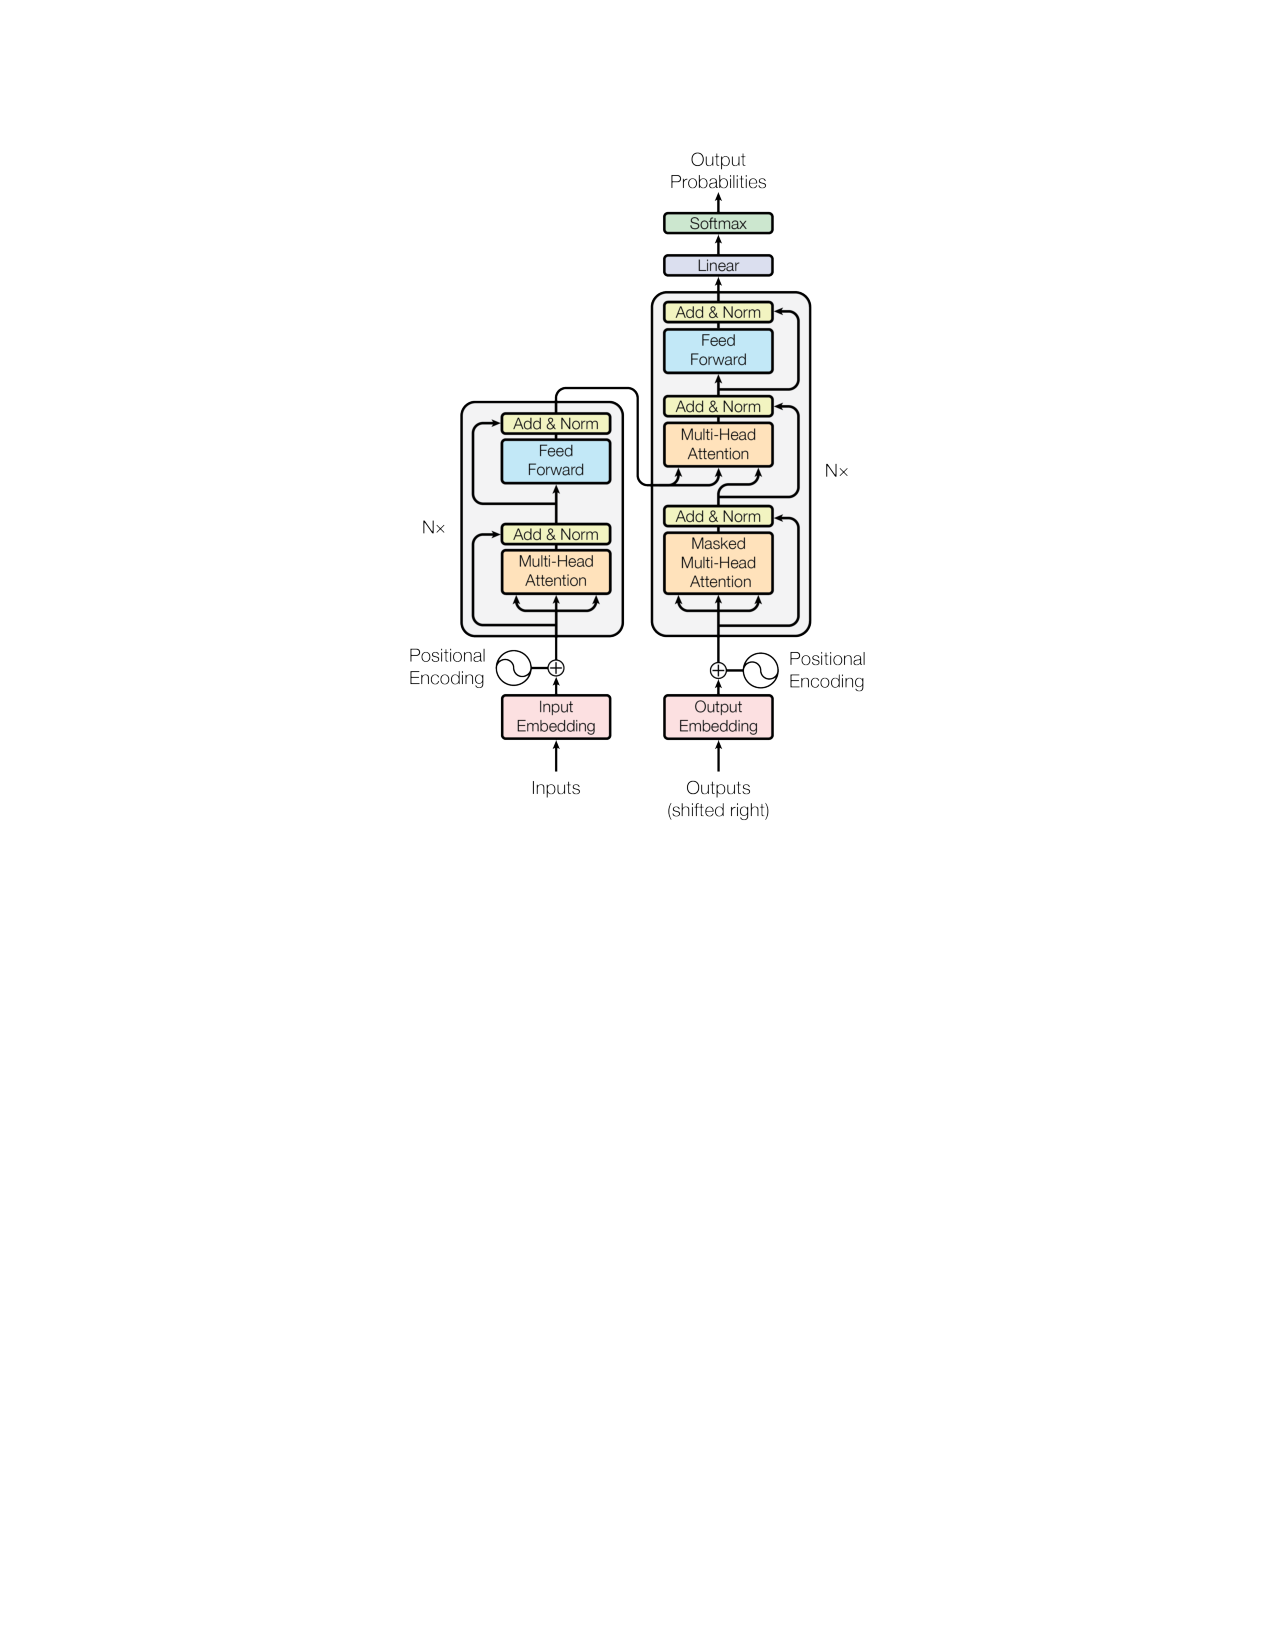
\includegraphics[width=10cm]{images/Transformer_architecture}}
        \caption[Figure of the transformer architecture.]{Transformer architecture proposed by Vaswani et al.\\
        Figure by Vaswani et al. \cite{vaswaniAttentionAllYou2017}.}
        \label{fig:transformer_architecture}
    \end{figure}


    
    %\subsection{Image Classification}


    %\subsection{Natural Language Processing}




% \section{Visual Question Answering}
    % What is VQA

    % Why is VQA important and interesting
    




\section{Model evaluation}
    In the field of machine learning and \gls{ai}, model evaluation refers to the process of measuring the quality and effectiveness of a trained model. These evaluations are essential in developing machine learning systems, allowing researchers and practitioners to determine their models' accuracy and generalization performance. Model evaluation helps to identify any weaknesses or shortcomings in a model's design or training process and enables researchers to make improvements to enhance the model's performance.

    \subsection*{Performance Metrics}
    \label{sec2:performance_metrics}
    Performance metrics are integral to machine learning models, allowing us to measure how well a model performs on a given task. These metrics evaluate the accuracy and effectiveness of a model's predictions by comparing them to the actual values. The choice of performance metrics depends on the problem being solved and the type of model being used. For example, in a binary classification problem, the model's accuracy can be used as a performance metric. In contrast, for multi-class classification problems, metrics like precision, recall, and $F_1$ score are more appropriate. In general, model evaluation metrics like precision and recall provide information about the performance of a model on a particular class, while accuracy and $F_1$ score provide an overall measure of model performance. Choosing appropriate performance metrics when developing a machine learning model is essential to ensure that the model's predictions align with the intended use case.
    
     % Precision and  Recall
    \subsection{Precision and Recall}
    Precision and recall are two important metrics used in classification tasks to evaluate the performance of a model. 
    Both precision and recall are based on the values in the confusion matrix, which is a table that summarizes the performance of a classification model. The confusion matrix contains four values: true positives, false positives, true negatives, and false negatives. True positives and false positives correspond to the model's positive predictions, while true negatives and false negatives correspond to the negative predictions. Figure \ref{fig:confusion_matrices} shows an example of a confusion matrix. The precision and recall are defined as follows.
        

    \begin{itemize}
        \item Precision: the ratio of correct answers among all answers proposed by the model, and it measures how precise the model's positive predictions are. The precision score can be calculated as follows:
        
        \begin{equation}
            \text{Precision} = \frac{\text{True Positive}}{\text{True Positive} + \text{False Positive}}
        \end{equation}
        
        \item Recall: the ratio of correct answers proposed by the model among all possible correct answers, and it measures how well the model is able to identify positive instances. The recall score can be calculated as follows:

        \begin{equation}
            \text{Recall} = \frac{\text{True Positive}}{\text{True Positive} + \text{False Negative}}
        \end{equation}
    \end{itemize}


    \begin{figure}[htb]
     \centerline{
         \begin{subfigure}[b]{0.5\textwidth}
             \centering
             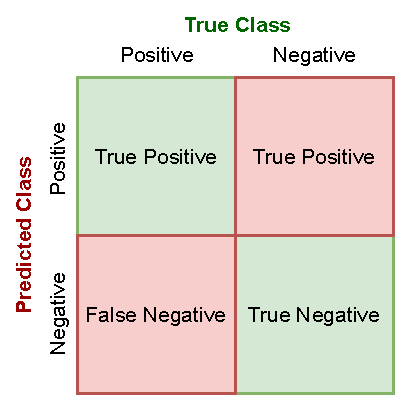
\includegraphics[width=\textwidth]{images/confusion_matrix_binary}
             \caption{Example of a confusion matrix of a binary classifier. A perfect classifier would have just true predictions.}
             \label{fig:confusion_binary}
         \end{subfigure}
         \hspace{0.1\textwidth}
         \begin{subfigure}[b]{0.5\textwidth}
             \centering
             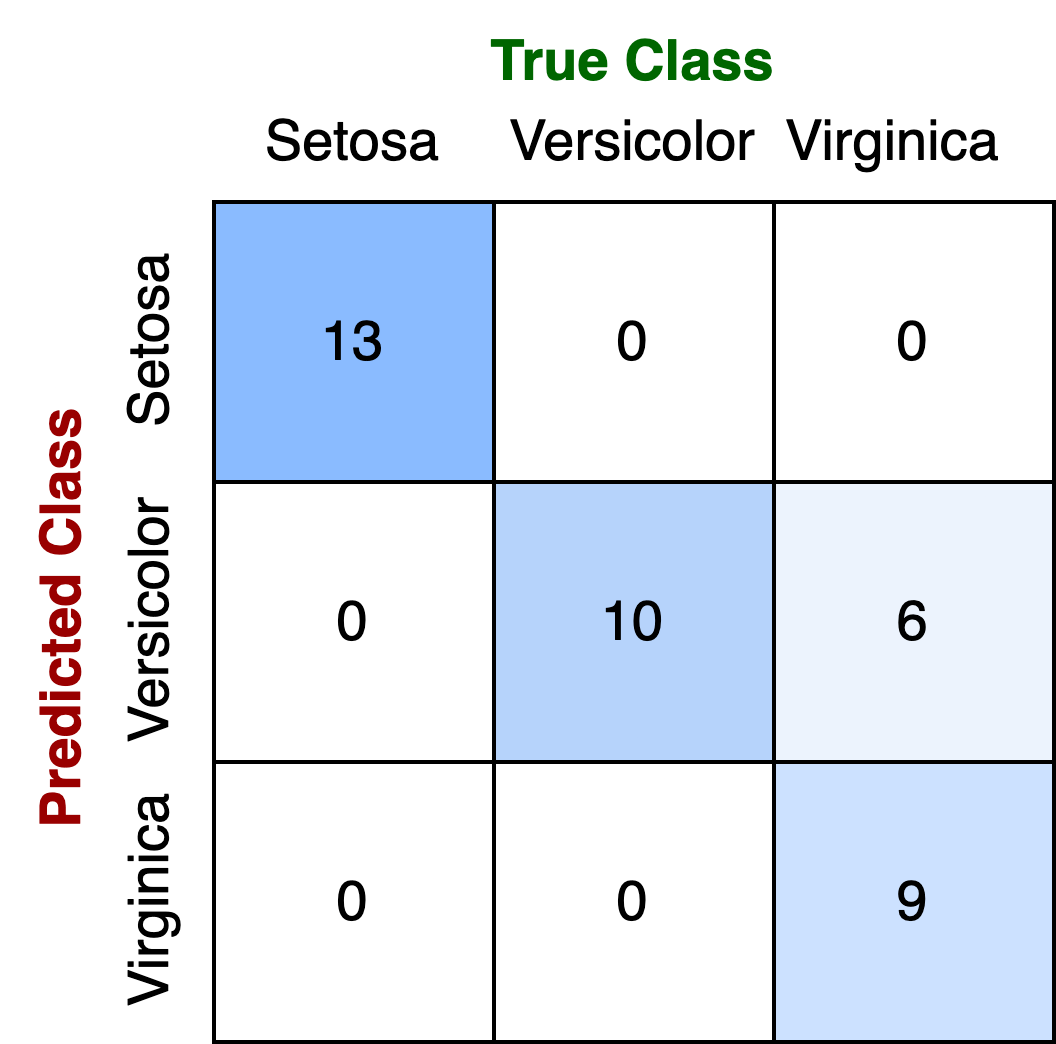
\includegraphics[width=\textwidth]{images/confusion_matrix_multi}
             \caption{Example of a confusion matrix of a multi-class classifier. An adapted example from scikit-learn \cite{ConfusionMatrix}.}
             \label{fig:confusion_multi}
         \end{subfigure}
         }
        \caption[Example of confusion matrices, both binary and multi-class.]{Example of confusion matrices, both for a binary (a) and multi-class (b) classifier.%Figure by the author.
        }
        \label{fig:confusion_matrices}
    \end{figure}


    % Accuracy
    \subsection{Accuracy}
\begin{comment}
https://www.statology.org/f1-score-vs-accuracy/
Accuracy:

Pro: Easy to interpret. If we say that a model is 90% accurate, we know that it correctly classified 90% of observations.

Con: Does not take into account how the data is distributed. For example, suppose 90% of all players do not get drafted into the NBA. If we have a model that simply predicts every player to not get drafted, the model would correctly predict the outcome for 90% of the players. This value seems high, but the model is actually unable to correctly predict any player who gets drafted.
\end{comment}
    Accuracy is a commonly used evaluation metric in statistics and artificial intelligence for classification models. It is a metric that is easy to interpret by humans because it measures the percentage of correctly predicted labels out of all the predictions made by the model. Accuracy is a valuable metric when the classes in the dataset are balanced, meaning that the number of instances for each class is roughly equal. However, when the classes are imbalanced, accuracy can be misleading. For instance, in a dataset with 95\% of the samples belonging to class A and only 5\% belonging to class B, a model that always predicts class A will have an accuracy of 95\% but will not be helpful in practice if the real-world data does not have the same distribution.

    Moreover, accuracy does not account for false positives and false negatives, as seen in Formula \ref{eq:accuracy}. False positives occur when the model predicts a positive label for a sample that is negative, while false negatives occur when the model predicts a negative label for a sample that is positive. In some applications, such as medical diagnosis, false negatives may be more costly than false positives, and accuracy alone may not be an adequate metric for evaluating model performance. Therefore accuracy can be a helpful and easily understandable metric when there is no critical downside predicting false negatives and the classes in the dataset are balanced. When dealing with real-world datasets, the classes are often not balanced, and a more suitable metric can be the $F_1$ score.
    


    \begin{equation}
        \text{Accuracy} = \frac{\text{True Positive} + \text{True Negative}}{\text{Total Sample Size}}
        \label{eq:accuracy}
    \end{equation}


    % F1 score
    \subsection{F\textsubscript{1} Score}


    The $F_1$ score is a statistical metric used to measure a model's performance on a dataset. It evaluates the performance of a binary classifier, which is a classification system that makes predictions for two possible classes, for example, positive and negative. The $F_1$ score can be calculated using the formula in Equation \ref{eq:f1}.

    \begin{equation}
        F_1 = 2 \frac{\text{Precision} \cdot \text{Recall}}{\text{Precision} + \text{Recall}}
        \label{eq:f1}
    \end{equation}

    In the context of question answering by an \gls{llm}, the $F_1$ score can be used to evaluate the accuracy of the model's responses to questions. Specifically, the score measures the harmonic mean of the model's precision and recall.

    \begin{comment}
https://www.statology.org/f1-score-vs-accuracy/
F1 Score:

Pro: Takes into account how the data is distributed. For example, if the data is highly imbalanced (e.g. 90% of all players do not get drafted and 10% do get drafted) then F1 score will provide a better assessment of model performance.

Con: Harder to interpret. The F1 score is a blend of the precision and recall of the model, which makes it a bit harder to interpret.

As a rule of thumb:

We often use accuracy when the classes are balanced and there is no major downside to predicting false negatives.

We often use F1 score when the classes are imbalanced and there is a serious downside to predicting false negatives.
    \end{comment}


    \subsection{Perplexity}

    Perplexity, often referred to as \textit{PPL}, is one of the most common metrics for evaluating language models. In information theory, perplexity measures how well a probability distribution or model predicts a sample. Intuitively, perplexity means being surprised, and in practice, it measures how surprised the model is when it sees new data. The lower the perplexity score, the better the training. Perplexity is usually only used to determine how well a model has learned the training set. 

    At its core, a language model is a probability distribution over a set of words, known as the model vocabulary. Considering all of its previous words, the model indicates the probability that a given word will appear in the vocabulary. Usually, the word with the maximum likelihood is selected as the next predicted word in the sequence.

    As an evaluation metric, perplexity can be used to compare probabilistic models, and low perplexity indicates that the probability distribution is good at predicting the sample. This probability can be calculated by multiplying a sequence of conditional probabilities for each word by its previous words, which indicates the probability of this sequence.
    Given a tokenized sequence $X = (x_0, x_1, ..., x_t)$, the perplexity of the sequence \textit{X} is given in the Formula \ref{eq:2_perplexity}.
        

    \begin{equation}
    \operatorname{Perplexity}(X)=\exp \left\{-\frac{1}{t} \sum_i^t \log p_\theta\left(x_i \mid x_{<i}\right)\right\}
    \label{eq:2_perplexity}
    \end{equation}

    In this formula, $\log p_\theta\left(x_i \mid x_{<i}\right)$ is the log-likelihood for the token with index $i$, given the previous tokens $x_{<i}$.

\section{Frameworks}
    %\subsection{PyTorch}
    This section briefly describes the most important external frameworks used in this thesis.
    
    \subsection{TensorFlow}
    
    TensorFlow is the framework used in the FLEX-VQA method proposed in this thesis. Here the framework is used to train the FLEX model to find connections between images and captions. A more detailed description of the implementation is discussed in Chapter \ref{sec:3_alpaca_vqa}.

    
    TensorFlow is an open-source machine learning framework developed and maintained by the Google Brain team. It was first introduced in 2015 and has since become one of the most widely used frameworks in machine learning.
    TensorFlow's core strength lies in its ability to handle large-scale machine learning models easily. It provides a highly optimized execution engine that efficiently computes complex models. This optimization is achieved through dataflow graphs, representing the computations as a directed graph of nodes and edges. Each node in the graph represents an operation, while the edges represent the data flow between operations. This architecture allows for parallelism and efficient computation, making it an attractive choice for large-scale machine learning tasks.
    
    One of the key advantages of TensorFlow is its versatility. It supports various machine learning tasks, including classification, regression, clustering, and reinforcement learning. It also supports deep learning models, such as \glspl{cnn}, \glspl{rnn}, and transformers.

    

    \subsection{Text Tokenization}
    \label{sec2:text_tokenization}

    Large language models such as GPT-3 \cite{brownLanguageModelsAre2020} and BERT \cite{devlinBERTPretrainingDeep2019} are trained on massive amounts of text data and can generate coherent and contextually relevant sentences, paragraphs, and even longer texts. However, feeding raw text data to such models can be computationally expensive and lead to suboptimal results due to high input variability. Therefore, text pre-processing techniques such as tokenization convert raw text into a form the model can more easily process.
    
    Tokenization is the process of splitting text into smaller units, called tokens, such as words, subwords, or characters. These tokens are then assigned a unique integer identifier and are often converted into fixed-length sequences, which can be fed into the language model. This process allows the model to handle text data more efficiently, reduces input variability, and helps to improve the training and inference times.
    
    Using a tokenizer specific to the language model used is crucial because it ensures that the tokens are consistent with the vocabulary and encoding scheme of the model. For example, using a tokenizer that splits words differently than the one used during the pre-training of the model can lead to inconsistencies and decreased performance.
    
    Various tokenization techniques are available, such as byte-pair encoding (BPE) \cite{gageNewAlgorithmData1994, sennrichNeuralMachineTranslation2016}, WordPiece \cite{devlinBERTPretrainingDeep2019}, and SentencePiece \cite{kudoSentencePieceSimpleLanguage2018}. BPE is a subword tokenization method that progressively merges the most frequent pairs of characters in a corpus to create a fixed-size vocabulary. WordPiece is a similar technique that uses a predefined list of subword units to tokenize words. SentencePiece is a more flexible method for creating a custom vocabulary that can handle rare and out-of-vocabulary words.
    
    Each of these techniques has its advantages and disadvantages. BPE and WordPiece are efficient and widely used, but they can result in a large vocabulary size and require additional processing steps to handle out-of-vocabulary words. SentencePiece can manage rare and out-of-vocabulary words better but can be computationally expensive due to their adaptive nature.

    This work uses a tokenizer built on top of SentencePiece, adapted and trained specifically to the \gls{llama} model. A more detailed explanation of this tokenizer can be seen later in \autoref{sec3:text_encoding}, which details the implemented method.
\label{sec:2_problem_and_application}
\section{Problem and application}
% Intro to this chapter

The increasing use of \gls{ai} has led to significant advances in various areas. However, understanding their decision-making processes becomes increasingly difficult as AI systems become more complex and opaque. 
The need for \gls{xai} and more transparent machine learning models has become imperative to address this problem, especially in applications where the consequences of wrong decisions can be severe, such as healthcare, finance, and autonomous vehicles. This chapter aims to provide an overview of the problem and application of \gls{xai}, which is crucial for building transparent and trustworthy \gls{ai} systems.


% Problem:
\subsection{Problem}
% ------------------------------------------

% Black-box
Although deep networks have made significant positive achievements in areas such as object detection \cite{girshickRichFeatureHierarchies2014, renFasterRCNNRealTime2015, redmonYouOnlyLook2016, linFocalLossDense2017}, image annotation and captioning \cite{vinyalsShowTellNeural2015, karpathyDeepVisualSemanticAlignments2015, johnsonDenseCapFullyConvolutional2016, tranRichImageCaptioning2016}, their complexity makes it more difficult to understand why these networks predict what they do. People, both researchers and users, of these systems need to be able to know how these black-box algorithms work to gain confidence \cite{koehlerExplanationImaginationConfidence1991, herlockerExplainingCollaborativeFiltering2000, dzindoletRoleTrustAutomation2003}, improve the models and apply these networks in new ways and domains \cite{jiangArtificialIntelligenceHealthcare2017, tonekaboniWhatCliniciansWant2019, holzingerCausabilityExplainabilityArtificial2019, guptaDeepLearningObject2021, tjoaSurveyExplainableArtificial2021}. Researchers and model architects can understand at a higher level how information flows in the network compared to everyday users by using their technical insight. However, as the architecture grows more profound and complex, and the training datasets are getting larger, it can be challenging to understand which parts of the input data contributed to making the decision \cite{sagirogluBigDataReview2013}.

% Interpretablity vs. accuracy 
\paragraph{Interpretablity vs. Accuracy\\}
The models with the highest accuracy for large data sets often have such complex architectures that even domain experts have difficulty interpreting their decisions \cite{caruanaIntelligibleModelsHealthCare2015}. Meanwhile, smaller, less complex architectures often have lower accuracy and generalize worse than their more complex counterparts. An example of this was shown in a case study to predict the risk of death for patients with pneumonia to help medical staff prioritize \cite{cooperPredictingDireOutcomes2005}. The researchers found the most accurate model to be a neural network, outperforming less complex models such as logistic regression. A rule-based system was also evaluated, and while this is a simpler model than neural networks, it is interpretable by design. This rule-based model to investigate the underlying dataset showed that a patient suffering from pneumonia and asthma had a lower probability of dying than only having pneumonia and was, therefore, less important to treat. The model drew this conclusion because patients in the training set with both pneumonia and asthma were usually prioritized first, was given medical treatment, and therefore had a higher survival rate \cite{cooperEvaluationMachinelearningMethods1997}. Because of this insight from the rule-based method, more complex models, such as neural networks, were concluded to be too risky in real-world decisions.

In pursuing models with higher accuracies, the primary way to achieve this is with even more complex models and larger training datasets \cite{bianchiniComplexityNeuralNetwork2014}. This brings the trade-off of an interpretable and explainable model vs. a more accurate model \cite{barredoarrietaExplainableArtificialIntelligence2020} to the forefront of discussion. 


% XAI
\paragraph{Explainable AI\\}
The field of \gls{xai} is working on solving the trade-off between performance and explainability. Some approaches specialize in explaining specific architectures, called model-specific. Meanwhile, others, called model-agnostic, try to explain models of different architectures, exploiting inherent properties in neural networks and statistics. Examples of inherently explainable models include decision trees, Bayesian classifiers, logistic regression, linear models, and \gls{knn} \cite{fixDiscriminatoryAnalysisNonparametric1989, coverNearestNeighborPattern1967, molnarInterpretableMachineLearning}. These algorithms are interpretable and, as a result of this, more explainable by design. This interpretability results from their internal structure, and computations follow clear rules or formulas that are manageable to comprehend.
However, models such as deep neural networks can work better than less complex methods on larger datasets. Because of their complex structure, with many hidden layers and weights trained on large datasets, it is difficult, if not impossible, for humans to understand what the model evaluated when choosing a prediction. Researchers in \gls{xai} have developed model-specific and \textit{post-hoc} model-agnostic techniques to understand better these complex methods to explain the underlying model prediction. The term post-hoc comes from Latin and means \textit{"after this"}. In this thesis, the term is used to describe a method applied after a machine learning model is developed. These methods try to bridge the gap between high accuracies and explainability.
In theory, this allows us to use the model best fit for the task, regardless of complexity, without the expense of not understanding the model's predictions. 

% Many models 
Different explanations try to give additional insights into the predictions. A local explanation looks at one specific model decision and tries to explain what was important in the input data to provide this prediction. A global explanation, on the other hand, looks at the whole model's process of making decisions and sees how the different attributes contribute to making a decision. These global explanations can also be built from multiple local faithful explanations. A third type is contrastive explanations that utilize local features to explain the difference between instances. This allows insight into the model's inner workings on a more global scale based on local predictions.

% Cons
One typical disadvantage of model-agnostic explanations is that their insights and descriptions are not always faithful to the underlying model they try to explain. This can happen if an explaining model is trained to look at the underlying model's input, inner workings, and output and learns the correlation between them. The problem is that correlation does not imply causation, and the explaining model can give a deceiving explanation that can look correct at first. Developing explanatory methods that find causations rather than correlations is an ongoing research topic.




% Application (where my system will go):
\subsection{Application}
% ------------------------------------------

% Intro
With better explanations that are intuitive and faithful to the underlying prediction model, humans can be more precise when improving the model. This also gives the ability to use the model with confidence that the prediction is based on correct decisions.


% Medical / bank
When machine learning methods are utilized as a tool in the real world, it is essential that everyone in the process of using the tool can trust the model. 
In a medical setting, both the doctor and the patient must have confidence that the conclusions drawn are based on a reasonable and trustworthy basis. If the model is correct, but the clinician does not trust the underlying model or the patient has no explanation for the model's conclusion, the model is not being used as intended and is, therefore, a useless tool.

This is also the case in other domains, such as finance. Here the bank can utilize large models that look at the loan applicant using big data. The bank can profile the customer alongside fellow citizens in the same demographic and use a model to predict whether or not that customer should receive a loan. In this case, finding all biases in the data set can be difficult, as it can be challenging to distinguish correlation from causation in demographic analysis \cite{garciaHarmsDemographicBias2019}. Here the bank must have an explanation alongside the predicted output of the loan to see better if the model made a trustworthy decision. 

% Non-experts improve models



% Finding bias in datasets
One advantage of better understanding the model's evaluations in a prediction is that it can highlight biases in the dataset. If these biases are known and understood, they can be combated. Ribeiro et al. \cite{ribeiroWhyShouldTrust2016} showed that it could be hard to discover biases when the predictions are correct without knowing the reasoning. They experimented with a model trained on images of huskies and wolfs and first presented the model's prediction without explanations to participants. The participants were then asked to determine if they trusted the model. Thereafter the model's explanation for the predictions was presented, and participants again had to tell if they trusted the model now. In both instances, the participants were also asked if they thought snow was a potential feature of importance. An image of a husky misclassified as a wolf can be seen in Figure \ref{fig:wolf_husky}, alongside the regions important in making the decision. The results can be seen in Table \ref{table:husky_vs_wolf}, and it can be seen that a considerable amount of the participants lost trust in the biased model when they were presented with the explanation. They then noticed that the decision was based only on whether the snow was visible in the image. This shows that models with an intuitive explanation are more likely to gain the trust of their users. Trustworthy explanations open the ability for users who do not have insight into the making of the model to still able to detect biases in the dataset and improve the model. 

\begin{table}[htb]
    \centering
    \begin{tabular}{ c c c} 
     
               & Before explanation & After explanation\\ [0.5ex] 
        \Xhline{1.5pt} \\ 
            Trusted the biased model & 10 out of 27 & 3 out of 27 \\  [0.5ex]
        \hline  \\ 
            Thought snow was an \\ important feature & 12 out of 27 & 25 out of 27 \\ [1ex] 
        \hline
    \end{tabular}
    \caption[Overview over the trust by participants in the "Husky vs. Wolf" experiment by Ribeiro et al. \cite{ribeiroWhyShouldTrust2016}.]{Overview over the trust by participants in the "Husky vs. Wolf" experiment by Ribeiro et al. \cite{ribeiroWhyShouldTrust2016}. The majority lost trust when explained that a classifier considered snow in the background the most important feature when classifying images of huskies and wolves.}
    \label{table:husky_vs_wolf}
\end{table}

\begin{figure}[htb]
    \centering
    \includegraphics[width=\linewidth]{images/husky_vs_wolf.png}
    \caption[Husky classified as a wolf, alongside an explanation of what the model considered important.]{Husky classified as a wolf, alongside an explanation of what the model considered important.\\ Figure by Ribeiro et al. \cite{ribeiroWhyShouldTrust2016}.}
    \label{fig:wolf_husky}
\end{figure} 


% Make humans able to learn from the models
Today's machine learning models are already better than humans in domain-specific tasks, like chess \cite{campbellDeepBlue2002}. Silver et al. \cite{silverGeneralReinforcementLearning2018} proposed the reinforcement learning algorithm AlphaZero, which learns to play chess, shogi (Japanese chess), and Go, only by playing with itself. This method does not get any domain knowledge except the game rules and achieves performance better than humans. Because this algorithm has not seen humans play these games, it does not have human biases and playing flaws in it, and professional game players can learn new moves and techniques by playing with it. 
As performance better than humans is a goal many researchers strive for when it comes to machine learning, it is more important than ever that these algorithms give explanations on what they do and why so that humans can learn new aspects never before thought of, as well as detect flaws that restrict performance, both in humans and machines.

\label{sec:2_related_work}
\section{Related Work} 

% Computer vision
% ------------------------------------------
\subsection{Computer Vision}
Computer Vision is the interdisciplinary task of making computers understand and act on visual input. This scientific discipline's main objective is to make computers extract high-dimensional data from the real world using digital images and videos. The extraction of visual information that computers can use includes methods for collecting, processing, analyzing, and understanding the images using statistics, geometry, physics, and learning theory. 

% Object detection
Object detection is a significant part of computer vision that has made astonishing progress. It has been an important research topic because it is one of the fundamental problems in computer vision. Detecting objects form the fundamental basis of other computer vision tasks, such as object tracking, segmentation, and image captioning. Many of these sub-domains' achievements have come from using \gls{cnn} architectures with more layers, trained on larger datasets, and more powerful computers. These main components have made the algorithms capable of learning a deeper understanding of the visual world and learning more fundamental elements of materials, objects, and scenes.  

% Is this relevant?
Krizhevsky et al. introduced AlexNet\cite{krizhevskyImageNetClassificationDeep2017}, as a variant of the \gls{cnn} proposed by LeCun et al.\cite{lecunHandwrittenDigitRecognition1989, lecunGradientbasedLearningApplied1998} seen in Figure \ref{fig:lenet}, both utilizing the backpropagation algorithm \cite{rumelhartLearningRepresentationsBackpropagating1986}
in training. The main difference is that AlexNet uses three more layers, ReLu \cite{fukushimaCognitronSelforganizingMultilayered1975}
, and is running on \glspl{gpu} instead of \glspl{cpu}, which in practice means more efficient use of computing power.
AlexNet achieved impressive results in the ImageNet \cite{dengImageNetLargeScaleHierarchical2009} 2012 Challenge and is often considered the most influential paper published in computer vision. 
Following this paper, there has been an increasing amount of work done and articles published in the domain of deep learning and images during the last decade.

\begin{figure}[htb]
    \centerline{
    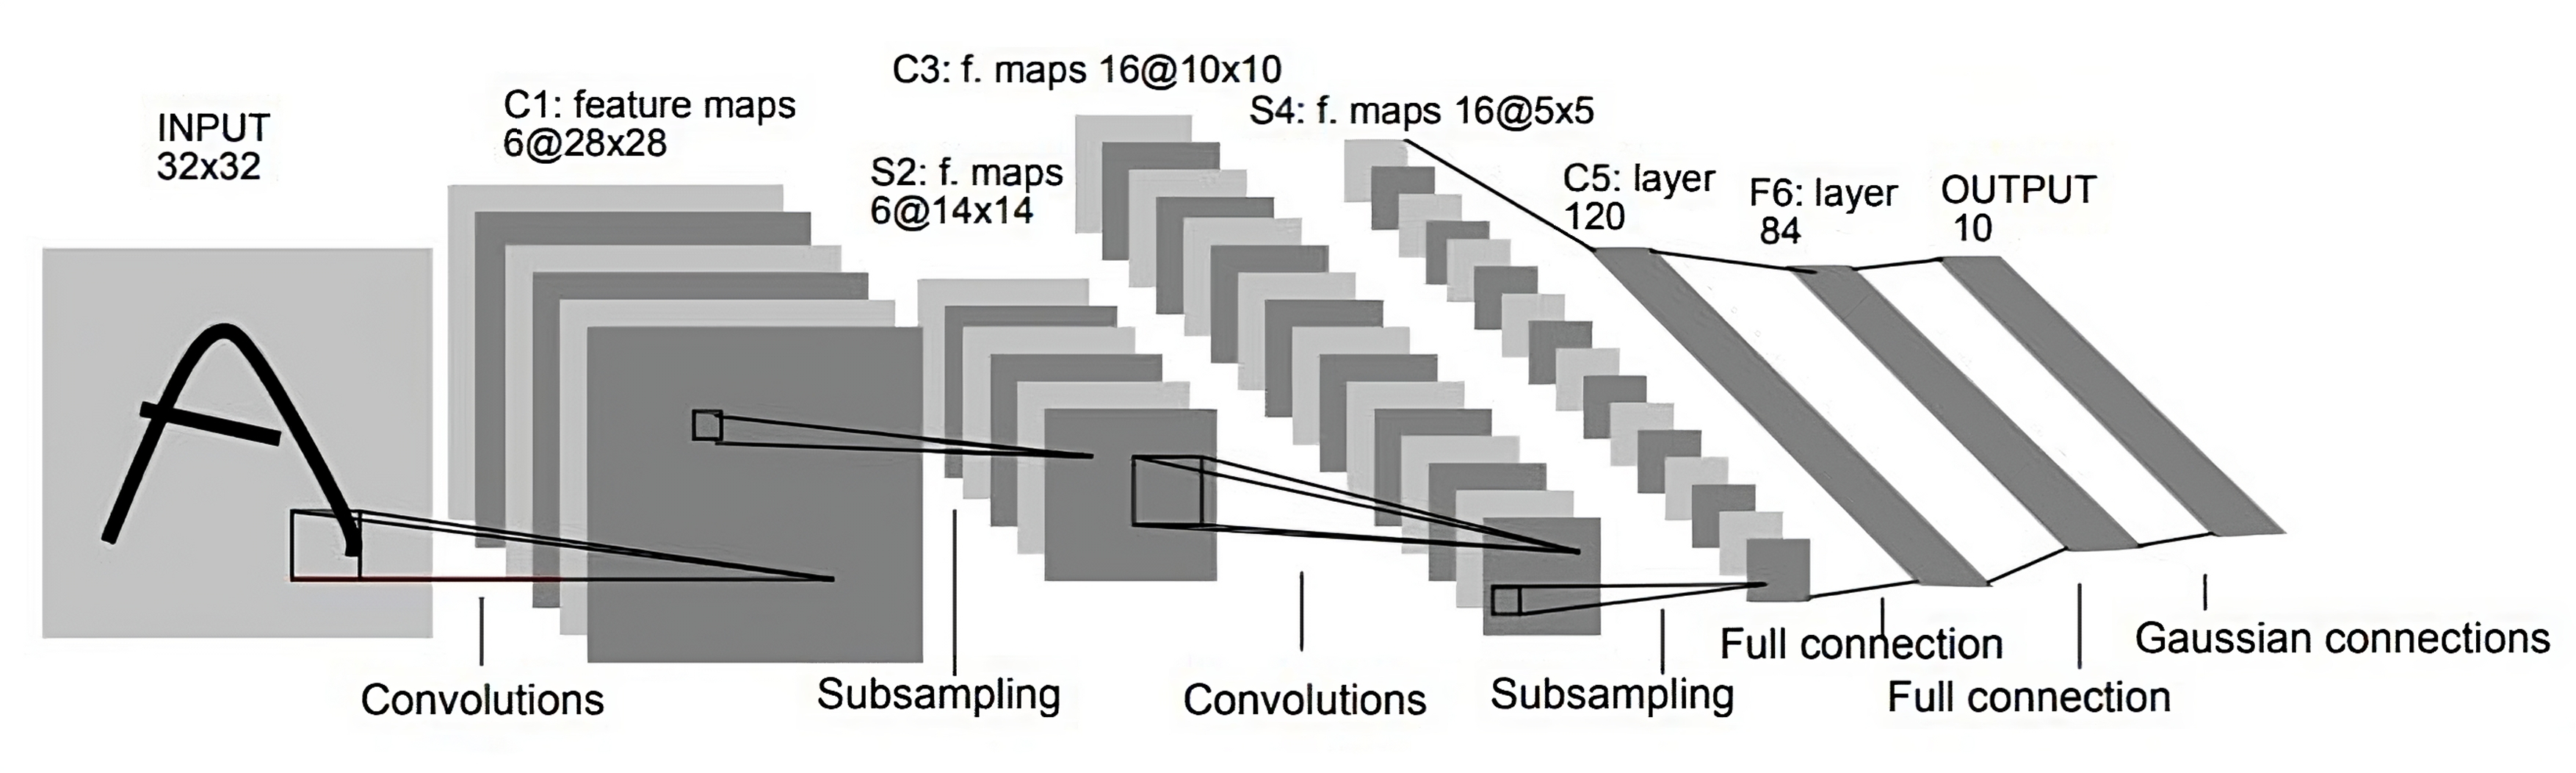
\includegraphics[width=1.2\linewidth]{images/LeNet.jpeg}}
    \caption{\gls{cnn} architecture of LeNet-5 proposed by LeCun et al. \cite{lecunGradientbasedLearningApplied1998}.}
    \label{fig:lenet}
\end{figure} 

% XAI
% ------------------------------------------
\subsection{Explainable AI (XAI)}

The rapid growth of artificial intelligence (AI) technologies has led to an increasing demand for transparency and interpretability in machine learning models. While these models have demonstrated impressive performance in various applications, their lack of transparency and interpretability has raised concerns about their reliability, accountability, and potential biases. As a result, the field of explainable AI (XAI) has emerged to address these challenges by developing techniques and tools that enable humans to understand how AI systems work and make decisions.

Explainable AI is an interdisciplinary research field that aims to make AI models more transparent, interpretable, and accountable to human users. It combines techniques from machine learning, human-computer interaction, cognitive science, and other related disciplines to develop methods and tools for explaining the behavior and decisions of AI models. The need for explainable AI arises from the fact that many machine learning models, especially deep neural networks, are often viewed as black boxes, meaning that their internal workings and decision-making processes are intricate for humans to comprehend. As a result, these models' lack of transparency and interpretability can create distrust among users, limit their adoption, and raise ethical concerns, especially in high-stakes applications such as healthcare, finance, and criminal justice.

An overview of influential methods proposed in \gls{xai} is presented in this subsection.

% LIME
\paragraph{LIME\\}
In pursuing a method that helps the explaining model to be locally faithful to the underlying model, Ribeiro et al. \cite{ribeiroWhyShouldTrust2016} proposed \gls{lime}. This model-agnostic method explains any method by learning an interpretable, less complex model locally around a specific prediction. This approach assures that the explanation is locally accurate and represents the actual inner workings of the model. 
In the same paper, they also introduce a method for explaining the global attributes of the model by framing the task as a submodular optimization problem. The technique is called SP-LIME (Submodular Pick LIME). With this approach, they can achieve global explanations that are locally accurate and faithful to the underlying model in a non-redundant way. LIME will be used later in this thesis as an explanation method adapted to a \gls{llm}.

% SHAP
\paragraph{SHAP\\}
Making non-redundant explanation features faithfully and efficiently is not easy. Lundberg et al. \cite{lundbergUnifiedApproachInterpreting2017} proposed a unified framework for interpreting predictions made by the underlying method. This framework called \gls{shap}, assigns each feature a value of importance for a specific prediction. The framework utilizes the class of additive feature attribution methods and estimates the Shapley % cite
values from cooperative game theory for that prediction. With this approach, they achieve more effective explanations to compute and have better consistency with human intuition than previously proposed methods.  


% Grad-CAM
\paragraph{Grad-CAM\\}
Visually explaining features that contributed to an image prediction can be essential in gaining trust in a model. Selvaraju et al. \cite{selvarajuGradCAMVisualExplanations2020} proposed a technique for making \glspl{cnn} more explainable and transparent by producing visual explanations for the underlying model. The method is called \gls{gradcam}, a generalization of CAM proposed by Zhou et al. \cite{zhouLearningDeepFeatures2016}, and uses the gradients in a single backtrack of any target concept. Therefore it does not need any architectural changes or retraining of the underlying prediction model to produce a localization map highlighting the crucial regions in the image for predicting the given concept, often called a saliency map in computer vision.

% DenseCap


% FLEX
\paragraph{FLEX\\}
While visual-only explanations can give the user insight into which areas of the image were essential in making the decision, they tell little to nothing about why those regions were important. On the other hand, linguistic descriptions give the user an essential understanding of the model's evaluation when predicting. 
Wickramanayake et al. \cite{wickramanayakeFLEXFaithfulLinguistic2019} propose \gls{flex} to merge saliency maps with locally accurate linguistic descriptions. In this approach, they look at the gradients through layers and identify the most critical activations in the single decision. The advantage of looking at different layers is that alongside getting an explanation that is faithful to the underlying model, they also extract features the \gls{cnn} identifies at each layer. A \gls{cnn} may represent high-level concepts, like a "car", at the last layer while identifying features such as texture and color at earlier layers. Using the activations at all essential layers, \gls{lime} achieves an image caption that explains all the essential parts of the prediction using sentences. \gls{flex} maps words to neurons in the \gls{cnn} by looking at high activations of that neuron combined with a word from the caption during the training. For this, they are using a \gls{cnn} and two stacked \gls{lstm} \cite{hochreiterLongShorttermMemory1997} cells.
The \gls{flex} framework is used as a basis for one of the two proposed methods in this thesis. A more detailed description of the specific implementation for this work is discussed later in Chapter \ref{sec3:flex_vqa}.

% VQA dataset
\paragraph{Visual Question and Answering (VQA)\\}
In order to make the linguistic abilities of computers more robust, Agrawal et al. \cite{agrawalVQAVisualQuestion2016} proposed a new dataset called \gls{vqa}. This dataset provides images from the COCO dataset \cite{linMicrosoftCOCOCommon2015}, paired with free-form, open-ended questions and answers corresponding to the content of the images. These questions and answers target different areas of the images, including underlying context and background details. This dataset aims to make models that can learn multi-modal visual and linguistic domain knowledge to get a more general and complete understanding of the world. Models that have done well in this dataset are frequently made up of \glspl{cnn}, to acquire the visual knowledge, combined with an \gls{rnn} % cite
for linguistic understanding.

Even though \gls{vqa} is not strictly \gls{xai}, it is still relevant regarding transparency to the user. \gls{vqa} is an important research area because it provides AI systems with human-readable explanations of their decision-making processes.
By providing a natural language explanation of why a specific answer was generated for a particular question about an image, \gls{vqa} models can help improve \gls{ai} systems' transparency and interpretability. This can be particularly important in domains such as healthcare and finance, where trust and transparency are critical for ensuring that \gls{ai} systems are making reliable and safe decisions. Therefore, it is important to continue developing and improving \gls{vqa} models to provide accurate and interpretable answers to questions regarding images.
Both the methods implemented and investigated in this work will be based on \gls{vqa}, using text to describe the contents of images utilizing different approaches.

\subsection{Large Language Models (LLMs)}

    \glspl{llm} are neural networks with billions or more parameters trained by self-supervised or semi-supervised learning on large amounts of text. They originated around 2018 and have performed competently on a variety of tasks. \glspl{llm} are typically general-purpose models that excel in various roles, with their performance and range of capabilities depending on the number of resources devoted during training. These models demonstrate considerable general knowledge about the world and can learn associations that make the model "memorize" numerous facts and contexts during training. 

    
    
    \glspl{llm} are pre-trained on large text datasets and can be characterized by four parameters: the size of the model, the size of the training dataset, the training cost, and the post-training performance. These variables are related by simple statistical laws called scaling laws. 

    \glspl{llm} serve not only to teach \glspl{ai} human languages but to understand proteins, write software code, and help students. These models are trained with vast amounts of text fed into the AI algorithm through unsupervised learning, allowing the model to find valuable connections in the language. Through this method, a \gls{llm} learns words, their relationships, and the concepts behind them. Large language models can also be tailored for specific use cases, including through techniques such as fine-tuning or prompt tuning, which feed the model small bits of data that must be focused on to train it for a specific application.
    
    
    However, a disadvantage of \glspl{llm} is that they can suffer from a phenomenon called hallucinations. Generative models can hallucinate because they contain vast amounts of data and organize the information in an unsupervised way. These models tend to make self-confident claims about facts not justified by their training data, which appears plausible but is not factually correct. Because of their size, they can also be challenging and computationally expensive to interpret. An ethical concern about the size of these models is that they are also computationally intensive during training and inference since they are trained on large datasets. As a result, these models have a larger carbon footprint than smaller models. However, there are ways to make these models smaller and faster, which are discussed in this chapter and also provide an overview of the development of large language models.

   

    \paragraph{BERT\\}

    BERT (Bidirectional Encoder Representations from Transformers) is a large-scale neural language model that has made significant contributions to the field of natural language processing (NLP) \cite{devlinBERTPretrainingDeep2019}. BERT is a pre-trained model that uses a transformer-based architecture that has grown in popularity in recent years due to its success in several NLP tasks. Introduced by Google in 2018, BERT is trained on a large corpus of text using an unsupervised learning approach. The model is pre-trained on a task called Masked Language Modeling (MLM), in which a small percentage of the words in a sentence are masked randomly, and the model is trained to predict the original word based on the context of the sentence. This method can be viewed as a "fill in the blanks" task, often called a cloze test, of the training sentences, keeping some words invisible to the model during training and helping the model generalize to new and unseen data. In addition, BERT is trained on an NSP task (Next Sentence Prediction), similar to the GPT models. The model is given pairs of sentences and asked to predict whether the second sentence continues the first.

    The main innovation of BERT is its ability to understand the context and provide contextualized word embeddings. Unlike previous word embeddings, which were static and did not change based on the context of the sentence, BERT can offer different embeddings to the same word depending on its context.
    
    
    
    \paragraph{BART\\}
    Lewis et al. at Facebook presented an \glspl{llm} named BART (Bidirectional and Auto-Regressive Transformer) \cite{lewisBARTDenoisingSequencetoSequence2019}. Like BERT, it uses a transformer-based architecture and is trained on a large corpus of natural language. However, unlike BERT, BART is unique because it integrates a bidirectional and auto-regressive architecture, which makes it well-suited for text generation and summarization tasks. 
    This model is a pre-trained sequence-to-sequence model that can be fine-tuned for various natural language processing tasks. BART is designed to handle auto-regressive, non-auto-regressive, generation, and comprehension tasks. The model is pre-trained on a large corpus of text using a denoising autoencoder objective, which requires the model to reconstruct original text from corrupted versions. Using a denoising autoencoder in pre-training helps reduce hallucinations by training the model to distinguish between real and fake input. 
    The authors demonstrate that BART outperforms several state-of-the-art models on various natural language generation and comprehension tasks, including summarization, question answering, and text classification. They also show that BART can be fine-tuned with relatively little data and can generalize to new domains. 
    However, instead of using Masked Language Modeling and Next Sentence Prediction like BERT, BART is pre-trained using a denoising autoencoder (DAE) objective.

    The DAE objective involves corrupting an input sequence by randomly deleting or swapping tokens and training the model to reconstruct the original sequence. This approach allows BART to handle more complex tasks such as text summarization, sentence generation, and machine translation.
        
    
    
    \paragraph{GPT\\}
    GPT (Generative Pre-trained Transformer) is a set of \glspl{llm} developed by OpenAI \cite{radfordImprovingLanguageUnderstanding2018}. Like BERT and BART, GPT is a transformer-based model but uses only an autoregressive architecture. It is pre-trained on large datasets and tuned for specific tasks. When GPT-2 was released, it was trained on a much larger dataset with significantly more parameters than GPT-1 \cite{radfordLanguageModelsAre2019}. This allowed it to generate more coherent and realistic text than its predecessor. GPT-3 is the third model in the GPT series and was released by OpenAI in 2020. It was trained on an even larger dataset than GPT-2 and had even more parameters, making it one of the largest language models. GPT-3 could generate even more readable and human-like text than its predecessors and perform various NLP tasks without explicit training \cite{brownLanguageModelsAre2020}. At the time of writing, the last published GPT model was GPT-4, which is still an autoregressive model but also includes multimodality \cite{openaiGPT4TechnicalReport2023} by making it able to interpret images. To reduce the effects of hallucinations on a generated output, GPT implements a combination of methods such as filtering and sampling.
    
    These models have proven to be versatile and powerful tools for natural language processing. GPT models have significantly influenced the NLP field, and many researchers and developers have used it as a starting point for their projects. Fine-tuned chatbot versions of GPT-3 and GPT-4 have been made available for public interaction under the name ChatGPT \cite{ChatGPT}.

    
    
    
    
    % LLaMA
    \paragraph{LLaMA\\}
    The \gls{ai} department of Meta, previously Facebook, released a modified architecture for a \gls{llm} called \gls{llama} \cite{touvronLLaMAOpenEfficient2023}.
    %This model with corresponding weights was not released to the public, but after a leak, \cite{vincentMetaPowerfulAI2023}, both the model and its weights became available to the public. 
    These models are created to compare to other \glspl{llm}, such as GPT-3 \cite{brownLanguageModelsAre2020}, Chinchilla \cite{hoffmannTrainingComputeOptimalLarge2022}, or PaLM \cite{chowdheryPaLMScalingLanguage2022}, while keeping the number of parameters considerably smaller. In the paper where Hoffman et al. propose the Chinchilla model, they also present insight into how models scale the best in conjunction with the size of the available dataset. The authors of \gls{llama} use this insight to make the model with fewer parameters perform well by training it on more tokens. The dataset that the \gls{llama} model is pre-trained on is publicly available and disclosed, which makes it compatible with open-source. The architecture is based on the transformer \cite{vaswaniAttentionAllYou2017}, with various improvements inspired by other \glspl{llm}. Some of these improvements are pre-normalization, inspired by GPT-3 \cite{brownLanguageModelsAre2020}, which improves the training stability by normalizing the input of each transformer sub-layer instead of the output. Like the PaLM model, they also use a SwiGLU as the activation function, first introduced by Shazeer at Google \cite{shazeerGLUVariantsImprove2020}, instead of ReLU. Shazeer showed it to improve the perplexities of transformer-based models. To make the self-attention mechanisms in the transformer position-agnostic, the authors implement a method called Rotary Position Embedding (RoPE) introduced by Su et al. This method allows both flexibilities of sequence length and faster convergence in fine-tuning compared to normal self-attention. With the 13 billion parameter version of \gls{llama}, the authors show that this model outperforms the GPT-3, with 175 billion parameters, on several evaluation metrics. Because the \gls{llama} model is ten times smaller than GPT-3, it can also be run on a single \gls{gpu}. These steps towards smaller, capable models benefit both the carbon footprint and inference compute budget and permit democratizing \glspl{llm} by making a model that can run on consumer hardware.

    \paragraph{Alpaca\\}
    The work in this thesis uses this Alpaca model to interpret images. More of how this model is implemented is discussed later in Chapter \ref{sec3:alpaca_vqa}.
    
    With Taori et al., Stanford University released an open-source fork of this \gls{llama} model, with some modifications, called Alpaca \cite{taoriStanfordCRFM, taoriStanfordAlpacaInstructionfollowing2023}. The Alpaca model is a fine-tuned model, with a 7B \gls{llama} model as the base model, trained on 52 thousand instruction-following tasks generated by OpenAI's text-DaVinci-003 model \cite{OpenAIAPI} using techniques from the Self-Instruct paper proposed by Wang et al. \cite{wangSelfInstructAligningLanguage2022}. Figure \ref{fig:alpaca_training} shows an overview of the Alpaca training procedure and how the dataset was built. By using text-DaVinci-003 to generate instructions, the team was able to train the model and generate the dataset for a significant cost reduction compared to traditional methods, totaling only \$600, with \$500 using OpenAI API to create the dataset and \$100 to rent 3 hours on 8 Nvidia 80GB A100 GPU cards. Reducing the cost of training an \gls{llm}, comparable to models much more expensive to develop, helps democratize these models and make them available to more people for less cost and energy.

    
    To address the ethical issue of not knowing whether a text is generated by an \gls{ai}, the team also implemented the method proposed by Kirchenbauer et al. \cite{kirchenbauerWatermarkLargeLanguage2023}. This method embeds "green" or marked tokens into the generated text, which are invisible to humans but can be detected by an algorithm analyzing a short span of these tokens.  
    The authors argue that the watermark can be embedded with negligible impact on text quality and can be detected with an efficient open-source algorithm without access to the language model API or parameters. The watermark works by choosing a random set of green tokens before generating a word and using a soft watermarking rule to encourage the input of green tokens during sampling. The authors propose a statistical test to detect the watermark with interpretable p-values and derive an information-theoretic framework to analyze the sensitivity of the watermark.

    Given the need for less computational resources, giving the method a reduced carbon footprint, and the ability to disclose the generated text as computer-generated, the Alpaca model represents a favorably ethical and transparent option for users of a system compared to other \gls{llm}. As such, it is an appropriate choice as a starting point for this thesis. This model has many of the benefits that \glspl{llm} can provide, like knowledge of vasts amount of data, while still being able to customize it to a specific task through fine-tuning. This process enables the model to adapt to a particular assignment while retaining the knowledge acquired from its initial training data.

    
    % Data flow
    \begin{figure}[htb]
        \centerline{
        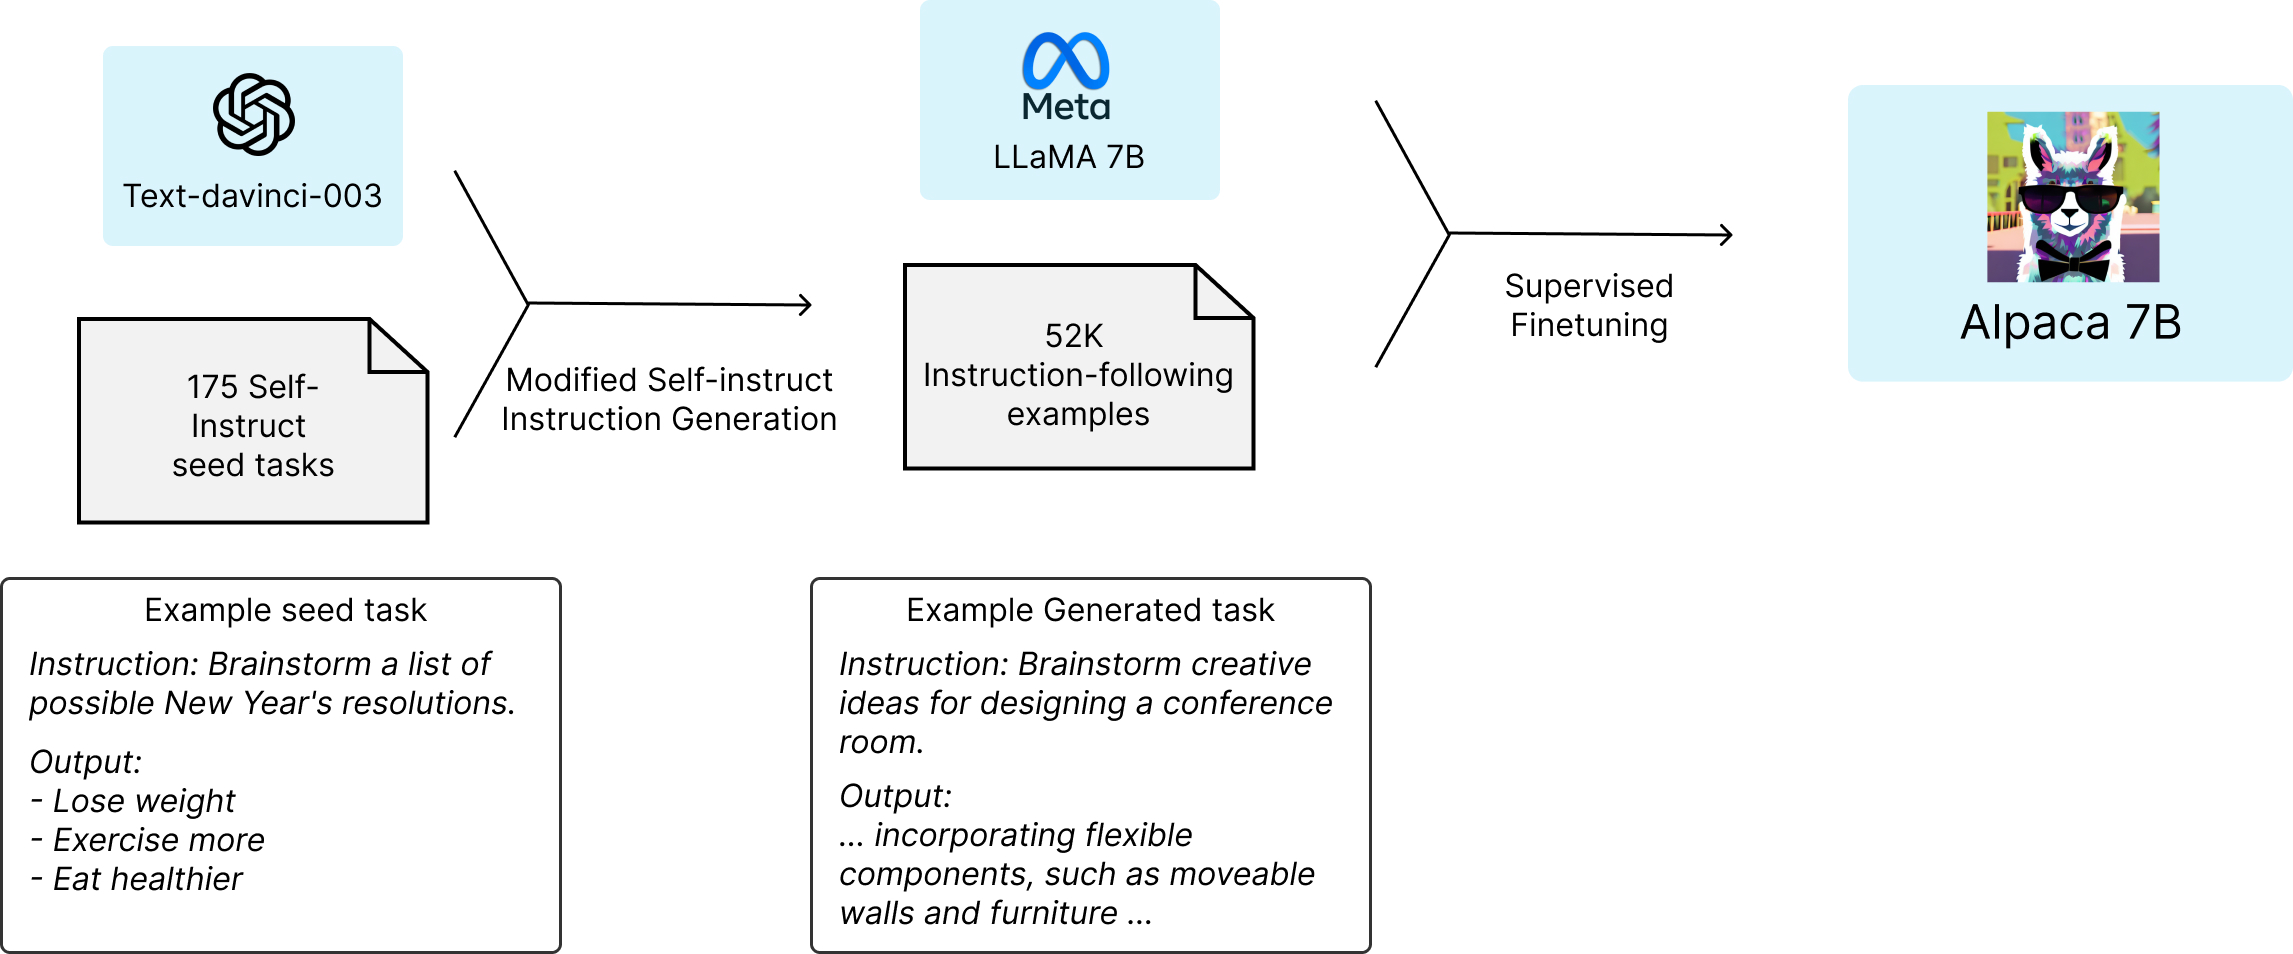
\includegraphics[width=17cm]{images/alpaca_framework.jpeg}}
        \caption[Overview of the Stanford Alpaca training procedure.]{Overview of the Stanford Alpaca training procedure.\\Figure credits: Taori et al. \cite{taoriStanfordCRFM}}
        \label{fig:alpaca_training}
    \end{figure}
\section{Summary}
\label{sec:2_summary}

\begin{comment}
SUMMARY: Often, we recommend ending this chapter (and all chapters after except the conclusion) with a summary section. The aim is to give an overview of, and tea-spoon-feeding the reader with, what he/she should have learned reading this chapter. What can be concluded from this chapter? How does the information given here give
 
arguments for your problem statement? Finally, lead to the next chapter (“... and we will therefore in the next chapter address these challenges, and describe our ideas/implementation/...”)
\end{comment}

\chapter{Methodology}
\label{sec:3_methodology}

\begin{comment}
This chapter may have many names. Lately, many have named it “Methodology”, but names like “Design and Implementation”, a “name” of a developed system, etc. are also often used. Just find a name that matches your research. Regardless, the important thing here is to describe YOUR research.

INTRO: Again, start the chapter with a sentence or two explaining why you have this chapter (repeating the last sentences from the proposed summary in the previous chapter) - assuming that some readers have not read the previous chapter.

MIDDLE SECTIONS: What are your ideas? Your solutions. How have you done “things”? Implementation details. Frameworks used. Etc. Also, discuss alternative ways of doing things and explain why you have chosen to do things as you have. WHAT! HOW! WHY!

SUMMARY: End this chapter with a summary section. Summarize what you have done and why! Main knowledge gained. What have we learned? Lead to the next chapter, stating that you will test your prototype.
\end{comment}


% INTRO:


% MIDDLE SECTIONS:
    % Implementation
    \section{FLEX-VQA}
        \subsection{Overview}
        % What:

        % FLEX
        There are two ways to address this task to make \gls{vqa} methods more transparent and explainable. Since the task has two modalities, namely vision, and language, the explanation can come from either the language model, the image model, or both. This thesis will address this task using the cross-modality explanation method \gls{flex} proposed by Wickramanayake et al. \cite{wickramanayakeFLEXFaithfulLinguistic2019}. An overview of the \gls{flex} model has been described shortly in sub-chapter \ref{sec:2_related_work} on page \pageref{sec:2_related_work}. This method is relevant for this thesis because it takes the explanation task to the visual module of the network and can generate an explanation for why a picture should be in a given class, using natural language. It combines a \gls{cnn} pretrained on the given task and does not need any training that modifies this pretrained image model when training to give explanations. An overview of the \gls{flex} framework can be seen in Figure \ref{fig:flex_overview}.

        \begin{figure}[htb]
            \centering
            \centerline{
            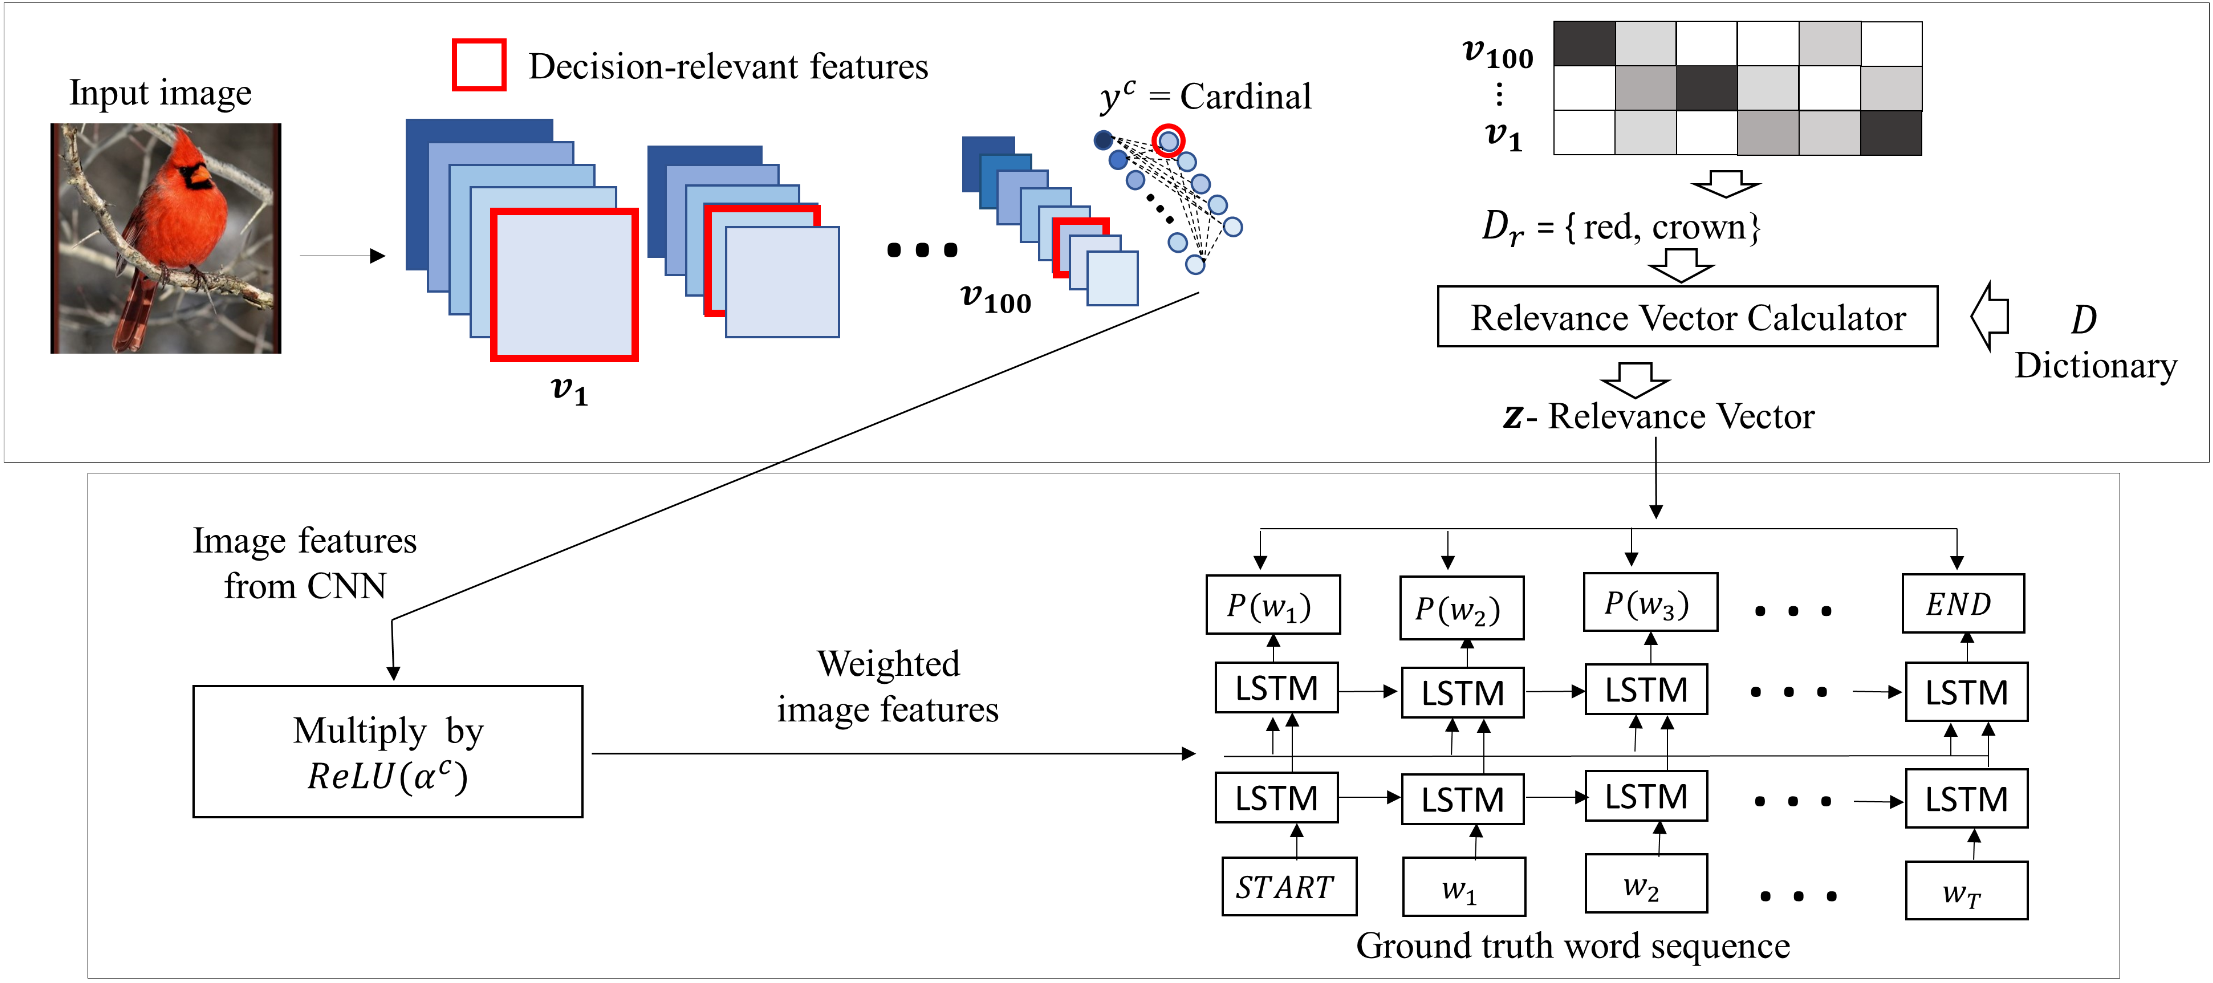
\includegraphics[width=17cm]{images/FLEX_overview.png}}
            \caption{Overview of the FLEX Framework.\\
            Image credit: FLEX framework proposed by Wickramanayake et al. \cite{wickramanayakeFLEXFaithfulLinguistic2019}.}
            \label{fig:flex_overview}
        \end{figure}

        % More in detail on how FLEX works. 
        Given an image and its predicted class $c$, the method finds a subset of the most important feature maps from each layer in the pretrained \gls{cnn}. To find the global activation score of each layer, it sums up each neuron in the layer, gives this score as an activation score, and then repeats for every layer. Thereafter it sorts the layers in order of importance and chooses a subset of $n$ layers so that the subset has combined importance over a chosen threshold. When a subset of the most important visual features is collected, \gls{flex} connects these visual features with linguistic features. The goal of using \gls{flex} is to find a connection score between a word ($w$) to every important element in the subset of feature maps ($F$) so that the word ($w$) best describes the important visual element ($v$) in each feature map. With a given ground truth description ($D_I$) of an image ($I$) in natural language, \gls{flex} uses this description for every image and builds a dictionary that contains all words in every description. This dictionary is called ($D$) and is used when describing new images, that do not have a ground truth description. For each word ($w$) \gls{flex} calculates co-occurrence score for each feature ($v \in F$), using the Dice score \cite{diceMeasuresAmountEcologic1945, sorensenMethodEstablishingGroups1948}. The word with the highest co-occurrence score gets associated with the visual feature ($v$). 



   
        This labeling of visual features can be reminiscent of DenseCap proposed by Johnson et al. \cite{johnsonDenseCapFullyConvolutional2016}, and Neural Baby Talk proposed by Lu et al. \cite{luNeuralBabyTalk2018}. The main difference between these methods and \gls{flex} is that \gls{flex} can be added to a network after the architecture is finalized, trained, and evaluated. In theory, it is agnostic to the underlying network, as long as the visual encoder has a property that allows it to find different parts of the network that correspond to different parts of an input image. \gls{flex} uses the \gls{gradcam} technique proposed by Selvaraju et al. \cite{selvarajuGradCAMVisualExplanations2020} to do a backward pass, through the feature maps of the \gls{cnn} to find the largest class activation maps when predicting a class. This information is then used to map words to important visual feature extractions in the network. This mapping of words combines the separable feature layers salient layers of the \gls{gradcam} method with natural language to make better explanations.


        \subsection{Implementation}
        % How:
        Given that \gls{flex} can combine information from the visual domain with natural language, it is an exciting framework to explore in the field of \gls{xai} and \gls{vqa}. A modified architecture to \gls{flex} is presented in this thesis, as seen in Figure \ref{fig:architecture_proposal}. This proposed architecture has unfortunately not been tested in this thesis, because of technical hurdles outside the scope of this thesis. A more detailed explanation of these hurdles can be seen in subsection \ref{subsec:no_flex}. However, since a lot of the available time for this thesis was put into researching this approach and finding the technical hurdles, until deciding that solving these hurdles was not relevant to this thesis, an overview of the architecture will still be proposed. 

       

        % Input from essay here.
        \subsection{Proposed architecture}
        
        Figure \ref{fig:architecture_proposal} shows how the data flow in the proposed method can work. It closely follows the \gls{flex} \cite{wickramanayakeFLEXFaithfulLinguistic2019} architecture proposed by Wickramanayake et al. It consists of a \gls{cnn} that extracts visual information and a 2-layered \gls{lstm} \cite{hochreiterLongShorttermMemory1997} \gls{rnn} that combine linguistic information with extracted visual features. This architecture is relevant for this thesis because it uses a backward pass to find locally accurate visual features, which are then used to give an image caption that describes what visual features were important to the classification and captioning of the image. This makes the architecture valuable as a starting point for this thesis and can be adapted to use \gls{vqa} datasets as linguistic input, to make it possible to ask questions regarding the classification of images and predictions. 
        
        % Explain the proposed data flow/architecture 
            % Training
            % CNN
        During training the proposed architecture takes an image and its corresponding questions and answers from the \gls{vqa} dataset. The images are fed through a \gls{cnn}-network, which can be pretrained on a larger dataset, like ImageNet \cite{dengImageNetLargeScaleHierarchical2009}. This is because the explaining method utilizes feature maps in each layer of the \gls{cnn}, so it is agnostic on what type of \gls{cnn} it is and what dataset it is trained on earlier. The \gls{cnn} predicts a class of what it sees in the image, and with a backward pass, finds important feature maps in each  convolutional layer. Each feature in the set of important feature maps gets associated with a word and stored in a relevance vector. This process is done by computing a co-occurrence score between each word in the ground truth caption and the feature. The feature with the highest co-occurrence score gets linked with that feature. 
        
            % LSTM
        The \glspl{lstm} gets trained by feeding each word in the ground truth caption into the first layer, alongside the hidden state of the \gls{lstm}. This is used to compute the next state, which gets concatenated with important visual features and is input to the second, and last, \gls{lstm}-layer. 
        The output from the second \gls{lstm}-layer is encoded to vocabulary space that is used to make a conditional probability distribution that later will be used to calculate the probability for predicting that word, given the given image features. 
        
            % Testing
        During prediction, the architecture takes an image and an optional question as input. The \gls{cnn} extracts important features in the layers, which get fed into the \gls{lstm}. Important feature maps from the \gls{cnn} are also used to calculate the relevance vector between features in the image and words. The \gls{lstm} uses this relevance vector, alongside important decision-relevant features from the image to predict a word. This word prediction is repeated until the stop word is predicted. 
        
        If no question is input to the algorithm during prediction, the model will use the most accurate predicted answer caption that describes the image as a whole as a caption for the image. On the other hand, if a question is submitted alongside the image, the \gls{lstm} will generate captions that answer the question asked, and then choose the most decision-relevant answer as the caption. 
        
        
        
        % Data flow
        \begin{figure}[htb]
            \centering
            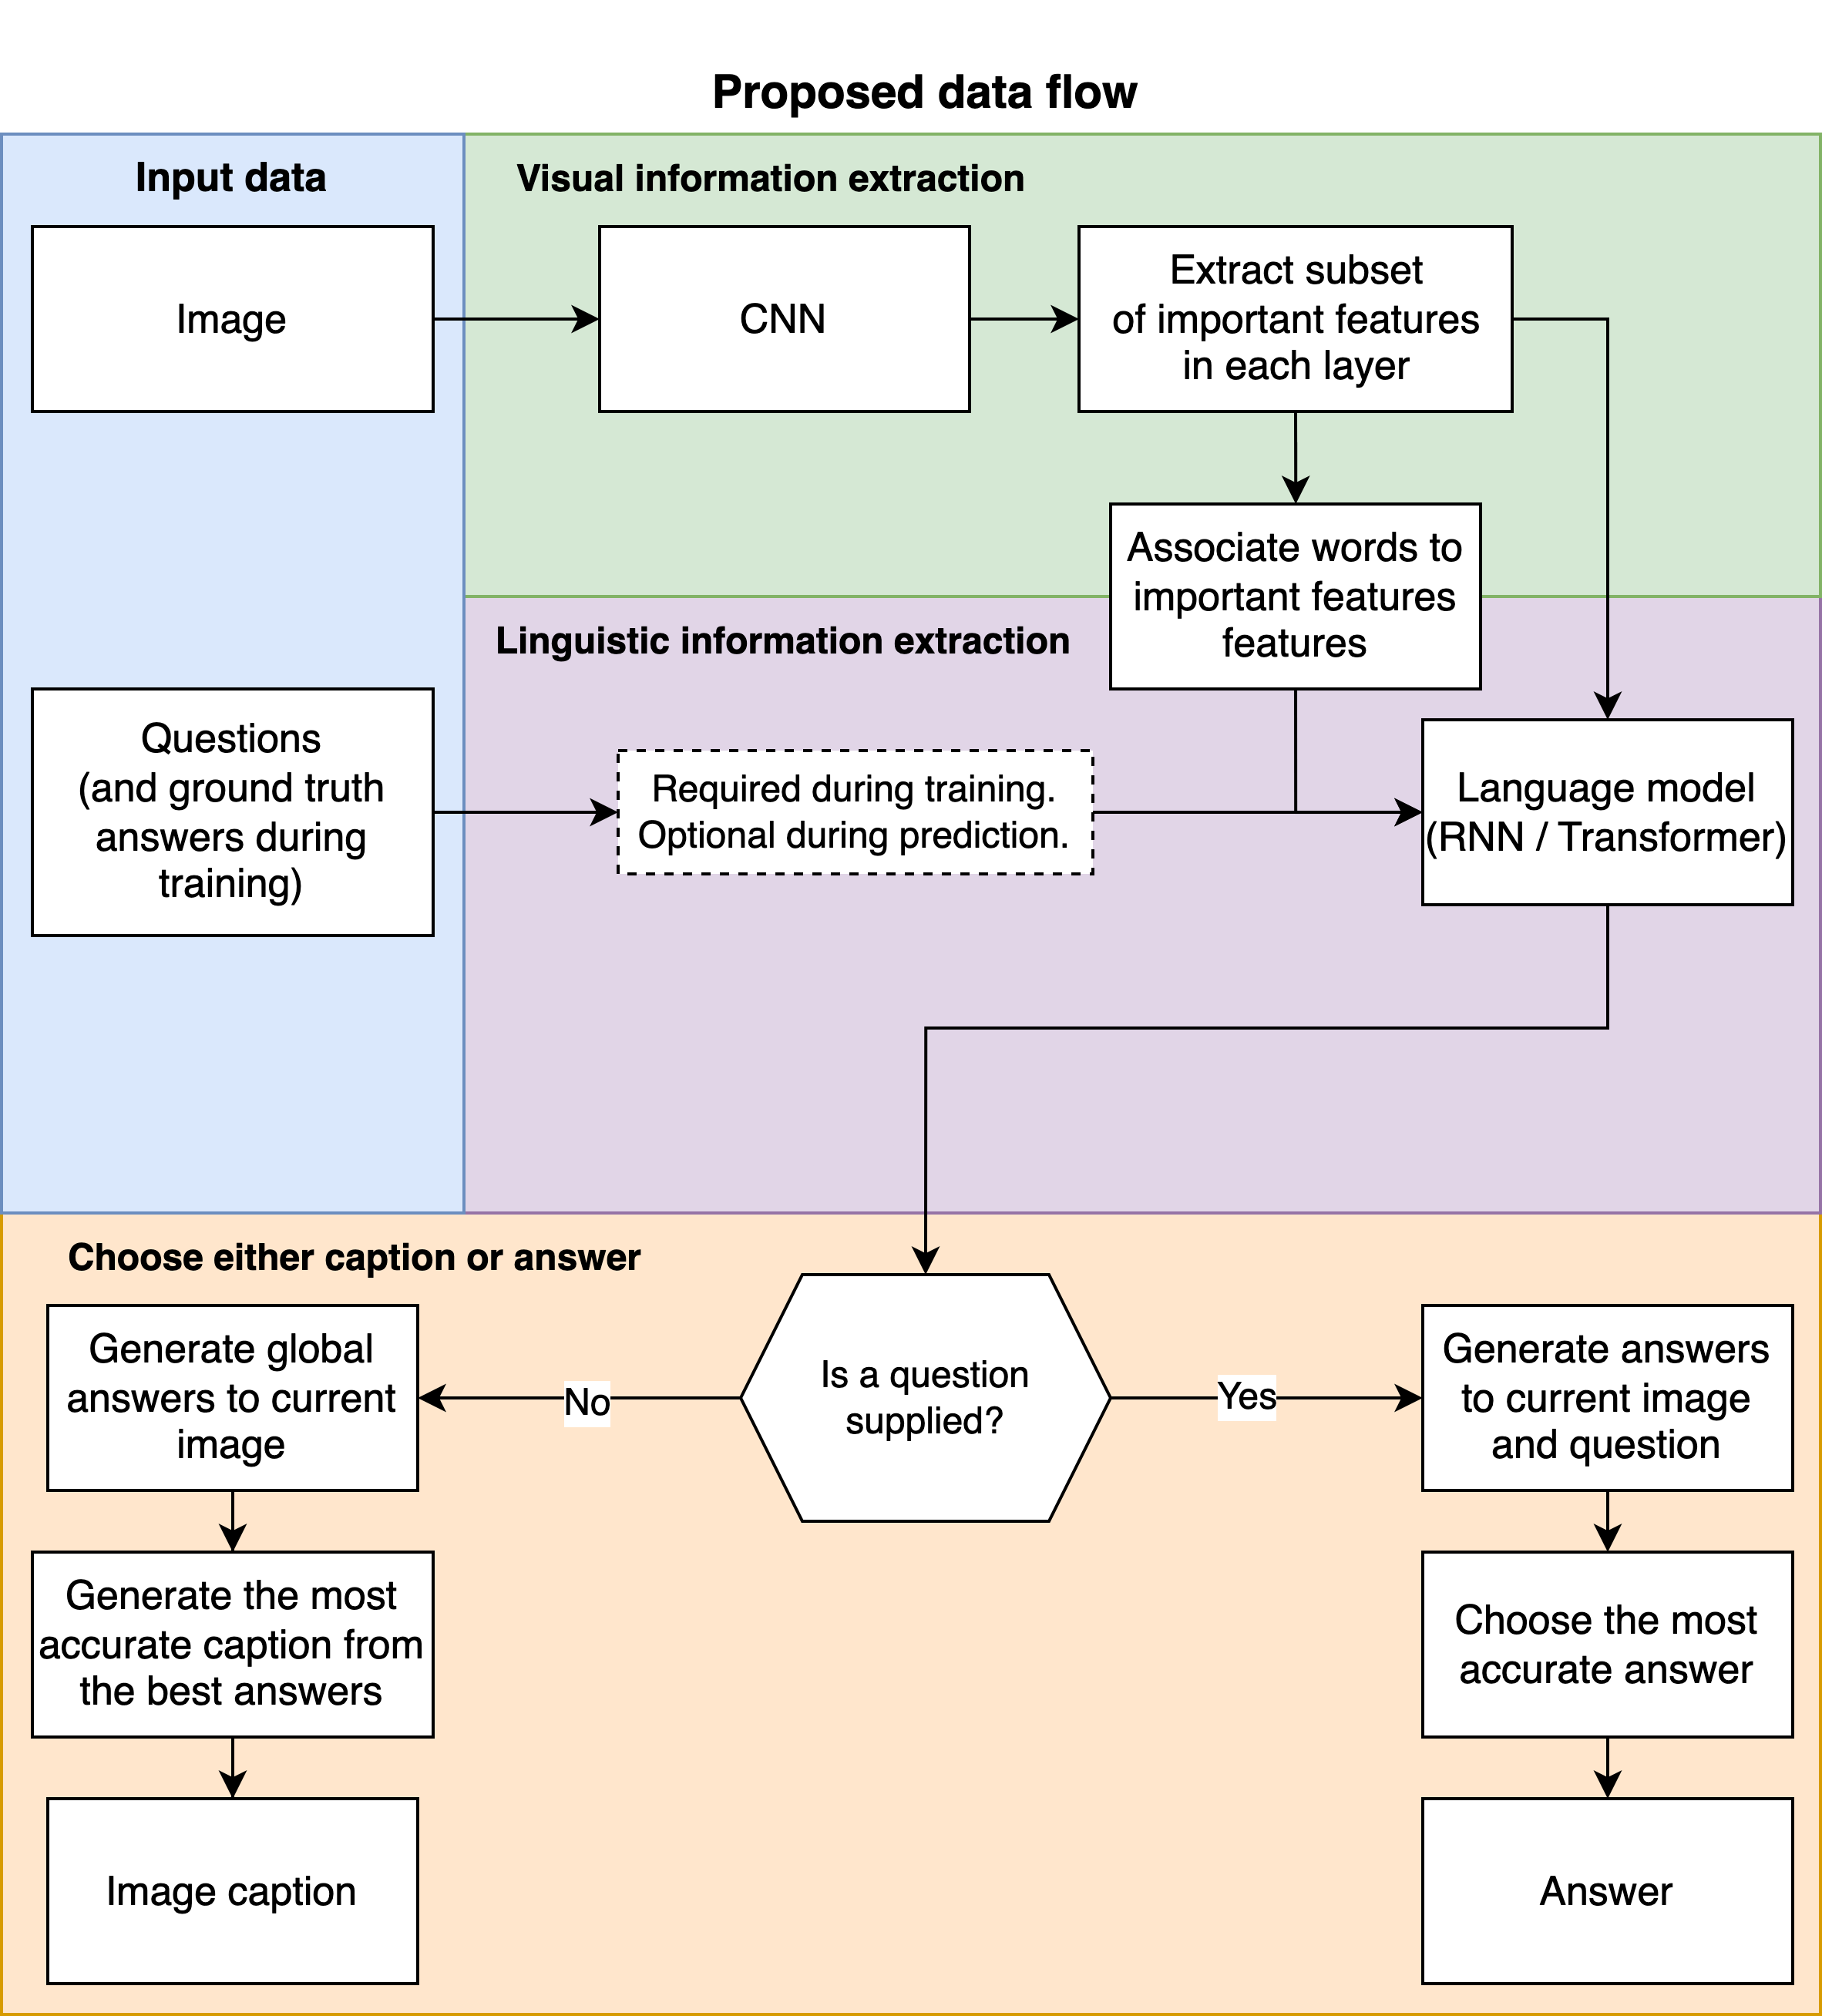
\includegraphics[width=\linewidth]{images/architecture_proposal.png}
            \caption{Proposal of the data flow and components that will be explored in this thesis.}
            \label{fig:architecture_proposal}
        \end{figure}
                
                
        

        % Why:

        By using \gls{flex} as a starting point, this thesis wants to explore how to make it able to be used for explainable \gls{vqa}. To adapt the \gls{flex} framework to \gls{vqa}, the dataflow shown in Figure \ref{fig:architecture_proposal} is proposed. Using this technique a user can get an answer for a question regarding an input image, that is both in natural language, faithful to the underlying \gls{cnn} model, and explainable. The explanation is faithful to the underlying model since it uses the actual gradients in the \gls{cnn} to find the words used in answering the question. This feature guarantees that if the underlying \gls{cnn} model has learned features that correlate with the answer, but are not the intended or logical features to pay attention to, these flaws get communicated to the user in natural language. Making a model that is able to explain what it weighs as important to a user, also when flawed, is important in making a system that a user can make a factually based decision in trusting or not. 

        Neither the \gls{cnn} nor the \glspl{lstm} needs to be specifically trained to be explainable. The architecture uses the underlying nature of the models to build an answer that is both transparent to the underlying model, as well as explaining to the user what the model values as important. 



        \subsection{Why this method has no experiments}
        \label{subsec:no_flex}

            % Intro
            To implement the proposed architecture, as shown in Figure \ref{fig:architecture_proposal}, it was natural to use the original code from the \gls{flex} paper as a starting point.
            The authors of the \gls{flex} paper also released the code used to do the experiments in the article. The experiments use an \gls{cnn} called Compact-Bilinear Pooling, which is a classifier proposed by Gao et al. \cite{gaoCompactBilinearPooling2016}. While the FLEX framework is designed to be model agnostic, the actual implementation of the experiments is tied closely with the \gls{cnn}, which has proven to be a hurdle when trying to both recreate the results in the paper and expand on the architecture and features. There main reason why this method has no complete experiments, nor results, is an outdated machine learning framework.
    
            
            \paragraph{The original implementation of FLEX\\}
            \gls{flex} need to be able to name feature maps in a given \gls{cnn}. This is an essential part of the framework and therefore needs to have insight into how the layers of the \gls{cnn} are structured.
            The implemented version of the original \gls{flex} architecture uses the Compact-Bilinear Pooling \gls{cnn}, which in short uses kernelization to reduce the number of dimensions of bilinear features to make it more computationally efficient, at the cost of having an architecture that deviates somewhat from the traditional \gls{cnn} architecture. The authors of the \gls{flex} paper, therefore, have implemented a version of the framework that addresses these special considerations when calculating co-occurrence metrics between words and features. 
        

            \paragraph{Why Caffe was needed\\}
            % Why Caffe was needed
            To use the same \gls{cnn} in a new context, as in this thesis, would require retraining or fine-tuning this network to suit the images in the given dataset. This would require the Compact-Bilinear Pooling model to train, or choose a new \gls{cnn} that could be merged with the \gls{flex} framework. The original Compact-Bilinear Pooling came with pretrained weights from training on the Caltech-UCSD Birds (CUB) \cite{PeronaLabCUB2002011} dataset. This dataset has images from Flickr and ImageNet but is solely focused on bird species and a rather small amount of images (11,788, compared to 14 million images in ImageNet \cite{dengImageNetLargeScaleHierarchical2009}). Therefore the original weights are best to classify this exact dataset but require retraining outside of this specific task.

            \paragraph{Getting Caffe to run\\}
            % Getting Caffe to run
            To get Compact-Bilinear Pooling to train on a new dataset, the underlying machine learning framework it was built in, had to be installed. This framework is named Caffe and is a deep learning framework developed by Berkeley AI Research (BAIR) / The Berkeley Vision and Learning Center (BVLC) and is a precursor to Caffe2, which was originally built by Facebook and merged with PyTorch. This forking and merging of newer versions of the Caffe framework have stagnated the development of the original Caffe framework, which has not received an update since 2017. The \gls{flex} framework itself is implemented in TensorFlow version 1.7, which at the time of writing is considered legacy. Because of the rapidly evolving nature of both software and hardware since 2017, it proved to be a nontrivial task to get Compact-Bilinear Pooling written in Caffe to run on the available hardware.

            To run the Caffe framework on \glspl{gpu}, to get the compute benefits necessary for deep learning, the framework supports \glspl{gpu} from Nvidia with \gls{cuda} version 5 through 8 \cite{CaffeInstallation, CaffeDeepLearning} and AMD \glspl{gpu}. The \glspl{gpu} in the compute cluster available to run experiments for this thesis are Nvidia RTX 2080 Ti, Nvidia A100, and AMD Vega 10 XL/XT, which run \gls{cuda} version 11.7, 11.5 and ROCm version 4.5.0 respectively \cite{MLNodesUniversitetet}. To not break compatibility with other services on the compute cluster, containerization was needed. Luckily containers are being actively deployed for Caffe with \gls{gpu} support, most notably from Nvidia and AMD.

            At the time of starting implementing the architecture described in Figure \ref{fig:architecture_proposal}, communication with the IT staff at the University of Oslo, responsible for the compute cluster available, was established. At that stage, only an experimental stage of containerization was available through the container engine Podman \cite{Podman}. In this container engine, the Nvidia container could not attach the Nvidia \glspl{gpu}. However, the AMD ROCm container could access the AMD \glspl{gpu} but did not have the correct driver compatibility to train the \gls{cnn}. Since Podman did not result in a container that could run successfully, a different container engine was installed, namely Apptainer, formerly known as Singularity. This new engine was able to see all the Nvidia \glspl{gpu}, but not the AMD ones. After the initial errors were ironed out, a Caffe container from Nvidia was successfully installed. Although successfully installed, the container had trouble running the training examples in the \gls{flex} code repository. While not a definite problem could be addressed because there were several different error messages. When the current error message was solved, a new one arose. The most likely explanation for the error messages was an incompatibility issue between the Caffe version in the container and the hardware it was tested on. After extensive testing and error-solving in seven months, the decision was taken that this technical problem was outside of the scope of this thesis, and this method was discontinued for this project. 
            

            
            \paragraph{How these problems could have been mitigated\\}
            % How this could be fixed.
            % implemented from scratch. 

            There are still some ways this method could be implemented. The main limitation of the chosen approach was to get the Caffe framework up and running, but there are still interesting ways to run experiments with the proposed method. Some proposed improvements based on the experience gained implementing this method are:

            \begin{itemize}
                \item \textbf{Remove Caffe from FLEX\\} 
                To have better compatibility with modern hardware and be more accessible to research moving forward, discontinued frameworks should be updated with more up-to-date versions. At the time of publishing the FLEX paper (2019), the development of the Caffe framework had already been stale for two years. To make research easier to peer-review, and implement by others, so that the proposed method can be further built upon, all researchers are served with publishing material that others can follow and implement themselves. By removing the Caffe framework from the FLEX framework, the method gets more accessible and easier to expand by others.
                

                \item \textbf{Update FLEX to TensorFlow 2\\}
                The FLEX framework is implemented in TensorFlow version 1.7, which was released in 2018. As of writing this thesis, TensorFlow versions 1.x are considered legacy. However, version 1.15, the latest version 1.x, is supported by TensorFlow 2. By updating to a more recent version, the framework can implement more modern features, gain compatibility with modern hardware and gain more users familiar with the current versions. This upgrade can both speed up the implemented FLEX framework through software and hardware optimizations, as well as speed up the development of the framework itself. 
                TensorFlow has migration guides and scripts to help translate from version 1 to 2 \cite{MigrateTensorFlowTensorFlow}, which makes the migration manageable. 
    

                \item \textbf{Make FLEX model agnostic in practice\\}
                The \gls{flex} framework is in theory separate from the \gls{cnn}. As proposed in the published paper, the implemented FLEX framework would benefit from being adapted to be agnostic to the underlying method. The originally implemented method has modified methods to extract image features from the specific \gls{cnn}. By using an agnostic implementation of the gradient search through the \gls{cnn} feature maps, the method could be expanded upon by allowing to test of different \glspl{cnn} to extract features and find co-occurrences with linguistic features. This could make the method more straightforward to implement for new \glspl{cnn}, which could make new methods more explainable.

            \end{itemize}

        % Outro / summary
        \subsection{Summary of FLEX-VQA}
        To summarize, by implementing the \gls{flex} framework into a \gls{vqa} method, the combined framework would make interpreting \gls{vqa} models easier and locally accurate. \gls{flex} has on a overall lever the same benefits as \gls{lime}, of being locally accurate. By having insight into a locally accurate explanation model, the method would make it possible for both researchers and users of an implemented system to see if the underlying model is trustworthy based on what the model deems important. 




    \section{Alpaca-VQA}

        \subsection{Overview}
        % What:
        To make a \gls{llm} that can see the world and explain what it sees, it was outside the scope of this thesis to train a model from scratch, both regarding time and resources. A \gls{llm} requires vast amounts of data when training, not only a large amount but also that it has good quality. Training the model requires large compute clusters that both consume lots of energy, cost much to facilitate, and produces greenhouse emissions \cite{??}. Therefore a \gls{llm} that was already pretrained was needed for this thesis, that further could be fine-tuned to answer the research goals. 

        Meta, previously Facebook, released a proposed architecture for a \gls{llm} called \gls{llama} \cite{touvronLLaMAOpenEfficient2023}. This model with corresponding weights was not released to the public, but after a leak \cite{vincentMetaPowerfulAI2023}, both the model and its weights became available to the public. Stanford University, with Taori et al., released an open-source fork of this \gls{llama} model, with some modifications, called Alpaca \cite{taoriStanfordCRFM, taoriStanfordAlpacaInstructionfollowing2023}. The Alpaca model is a fine-tuned model, with a 7B LLaMA model as the base model, trained on 52 thousand instruction-following tasks generated by OpenAI's text-DaVinci-003 model \cite{OpenAIAPI} using techniques from the Self-Instruct paper proposed by Wang et al. \cite{wangSelfInstructAligningLanguage2022}. An overview of the Alpaca training procedure can be seen in Figure \ref{fig:alpaca_training}. By using text-DaVinci-003 to generate instructions, the team was able to train the model  and generate the dataset for a significant cost reduction, totaling only \$600, with \$500 using OpenAI API to generate the dataset and \$100 to rent 3 hours on 8 Nvidia 80GB A100 GPU cards. This reduction in the cost of training an \gls{llm}, comparable to models much more expensive to develop, helps democratize these models and make them available to more people for less cost and energy.
        To address the ethical issue of not knowing whether a text is generated by an \gls{ai}, the team also implemented a method proposed by Kirchenbauer et al. \cite{kirchenbauerWatermarkLargeLanguage2023} which embeds "green" or marked tokens into the generated text, which are invisible to humans but can be detected by an algorithm analyzing a short span of these tokens.


        % Data flow
        \begin{figure}[htb]
            \centerline{
            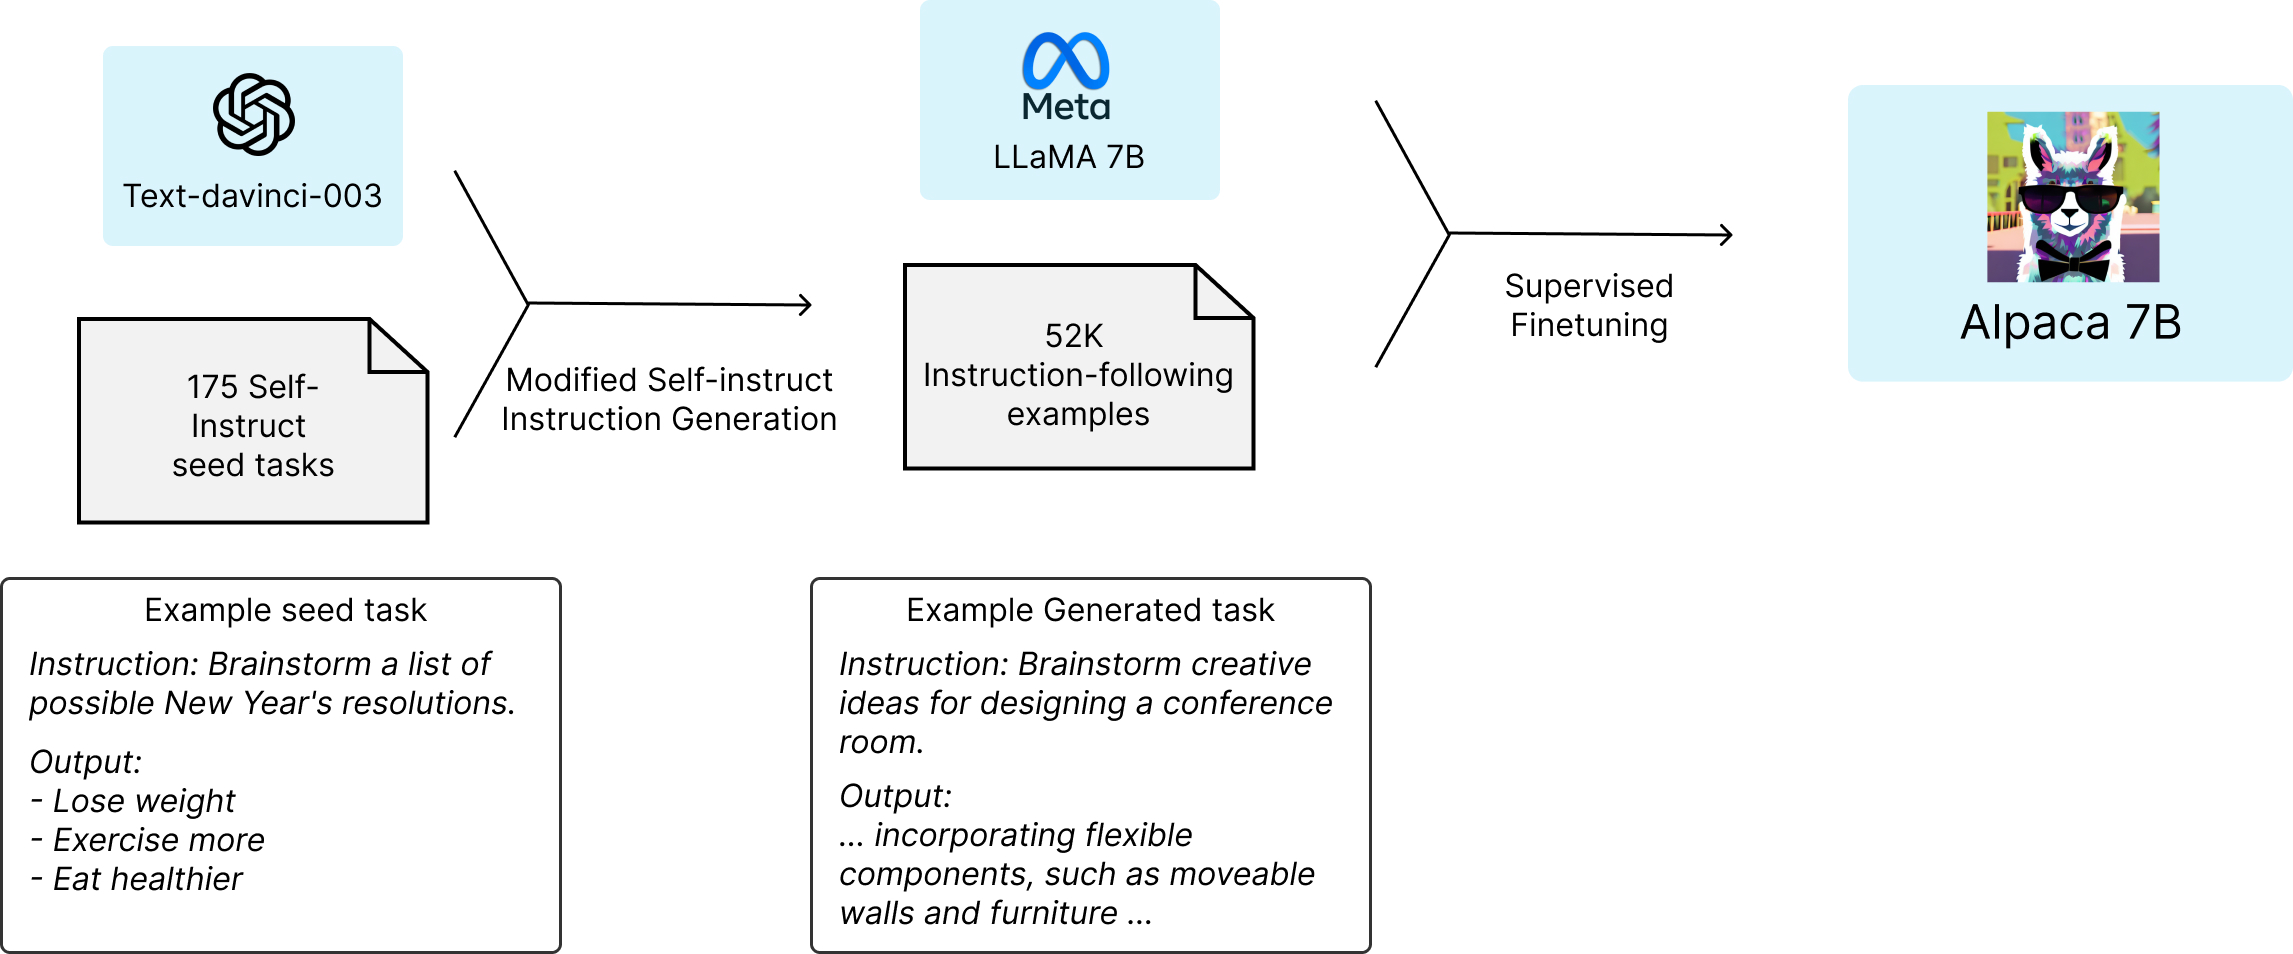
\includegraphics[width=17cm]{images/alpaca_framework.jpeg}}
            \caption[Overview of the Stanford Alpaca training procedure.]{Overview of the Stanford Alpaca training procedure.\\Image credits: Taori et al. \cite{taoriStanfordCRFM}}
            \label{fig:alpaca_training}
        \end{figure}


        % Alpaca-LoRA
        Even though the Stanford Alpaca model was trained using significantly less computing power compared to other \glspl{llm}, it is still advantageous to further lower the necessary compute budget to train and fine-tune models. A technique that was proposed by Hu et al. called \gls{lora} \cite{huLoRALowRankAdaptation2021} addresses this issue. The way they address this task is to add pairs of rank-decomposition weight matrices, commonly referred to as update matrices, on the existing weights and only train these newly added weights. This has many advantages, most importantly accelerating the training while reducing memory consumption. Other advantages of these added matrices are that the original weights are kept frozen, which makes the \gls{lora} model not as prone to catastrophic forgetting. The added weights are also typically less than 10 percent of the original trainable parameters, making it more feasible and faster to train domain-specific models that can change the smaller \gls{lora} weight matrices on the fly to more accurately answer a task. When using \gls{lora} matrices, they also allow both training and interference on consumer hardware, like desktop \glspl{gpu} and even single-board computers like Raspberry Pi's \cite{artemandreenko[@miolini]VeSucefullyRunned2023}. 


        \subsection{Implementation}
        % What I did implement
        To address the research questions stated in \ref{sec:1_2_problem_statement}, considering ??, a \gls{lora} version of the Stanford Alpaca version was used to carry out the experiments. The code used as a starting point is a fork of Erik J. Wang's Alpaca-LoRA \cite{wangAlpacaLoRA2023}, which was further modified to fit this thesis' experiments. The most notable modification to this model is to make it cross-modal, by allowing it to take both text and images as input.

        \subsubsection{Make a language model see images}
        % How to get the model to see
        To make the model able to interpret images, an image encoder had to be implemented. To make the \gls{llm} able to do the interpretation of image data, the visual features had to be extracted in a manner that allowed it to be fused with the text input. Also, to make it more efficient to experiment with different image encoders, a dataflow that first finds an image-to-text feature, that is incorporated into the text input prompt to the language model. In Figure \ref{fig:alpaca_vision} the proposed dataflow is shown. This architecture allows the language model to be agnostic to the image encoder, which allows it to use a fine-tuned \gls{cnn} or vision transformer for a specific task. 

        % Data flow
        \begin{figure}[htb]
            \centerline{
            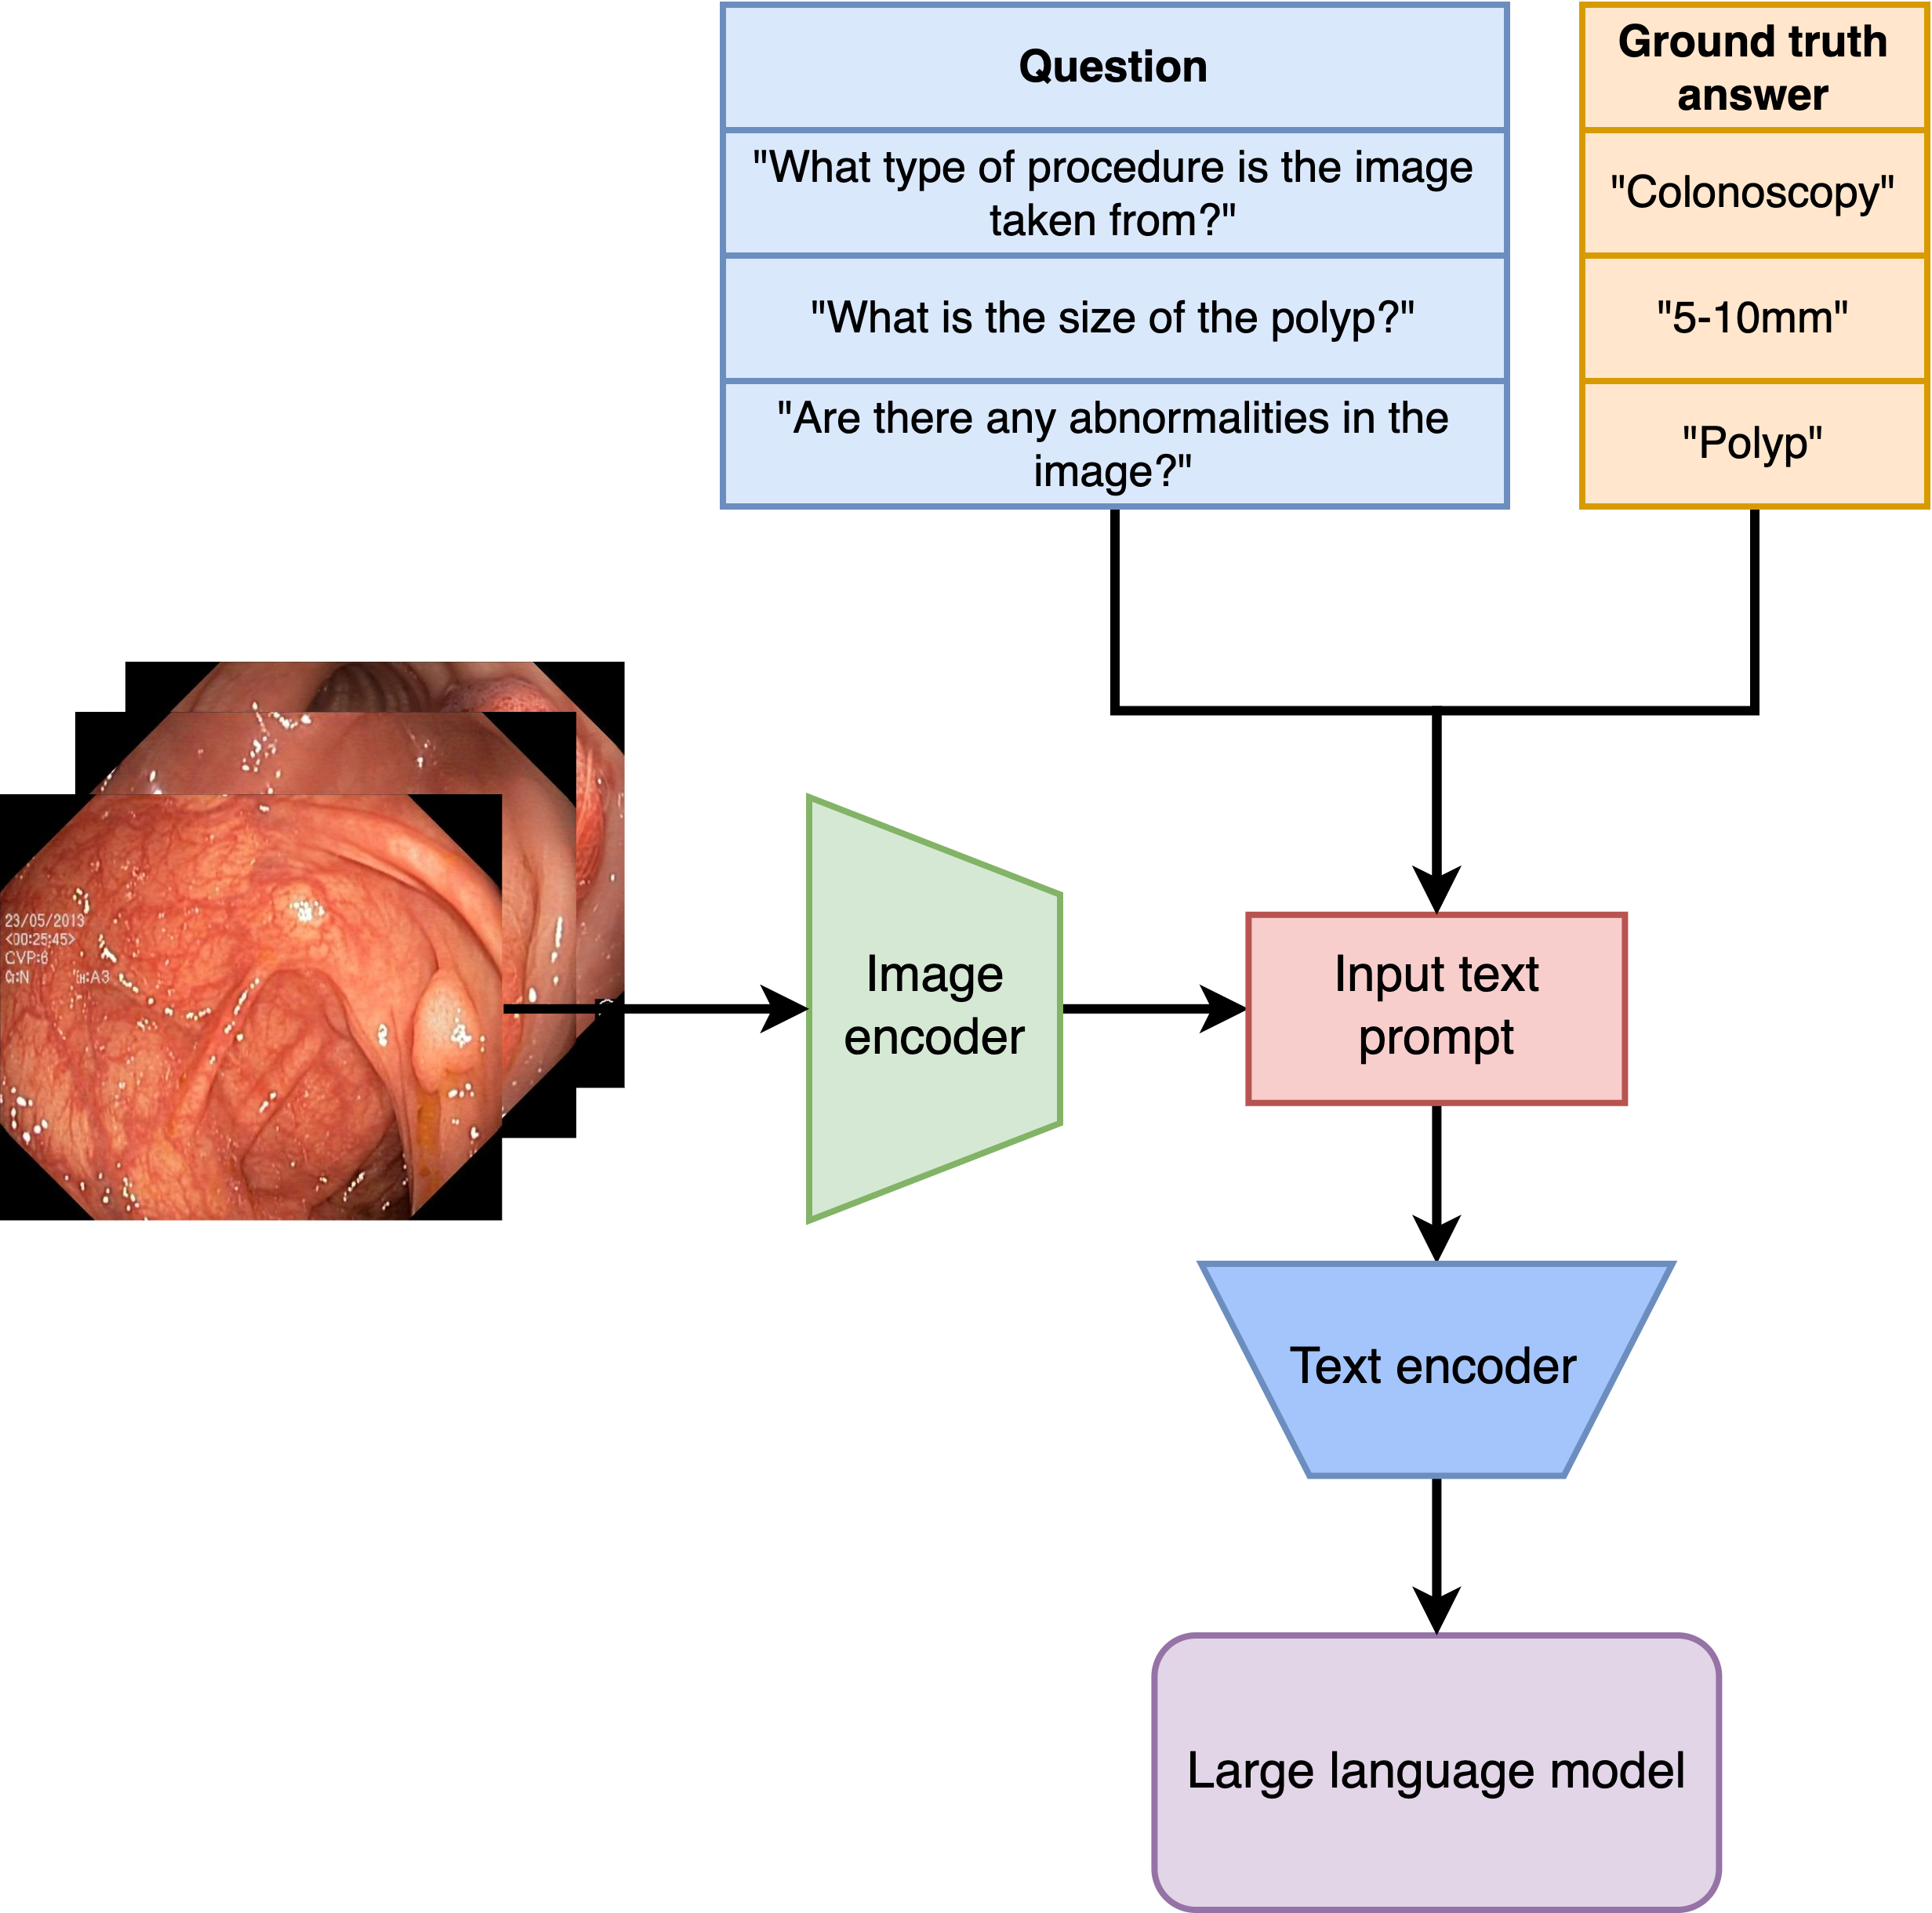
\includegraphics[width=\textwidth]{images/alpaca_vision.png}}
            \caption[Overview of the proposed dataflow to make large language models interpret images.]{Overview of the proposed dataflow to make large language models interpret images. The images represented in this Figure are from the HyperKvasir dataset by Borgli et al. \cite{borgliHyperKvasirComprehensiveMulticlass2020}.}
            \label{fig:alpaca_vision}
        \end{figure}


        % How & Why :
        Specifically, the image encoder first implemented was \gls{vgg}-16, proposed by Simonyan and Zisserman at Oxford \cite{simonyanVeryDeepConvolutional2015}. The rationale for implementing this \gls{cnn} first, is that it’s a well-known network, which also achieves relatively good performance on the ImageNet dataset, with 92.7\% on the test set. The VGG-16 model used for the initial experiments is pre-trained on the ImageNet \cite{dengImageNetLargeScaleHierarchical2009} dataset. The model would most presumably perform better if pretrained on the specific dataset used, namely the HyperKvasir dataset \cite{borgliHyperKvasirComprehensiveMulticlass2020} made by Borgli et al. However, the initial experiments will try to explore the feasibility of the proposed approach, rather than achieve optimal accuracy.

        % Explain why VGG-16 should work even if it does not give regions of interest
        Given that the VGG-16 network is pre-trained on ImageNet, it outputs a probability for each of the 1000 classes in the dataset. To address the task of extracting features from any image, regardless of if the \gls{cnn} is pretrained on the task, the method implemented extracts the top 100 ImageNet highest probability classes. With this approach, the image feature extraction will find a consistent amount of features in an image, sorted with the feature with the highest probability first. The features with the highest probability are the features most likely to have a feature map similar to a class in ImageNet. Therefore, even if the class label from ImageNet is not connected with a correct label from the HyperKvasir dataset, there is a high probability that the feature extraction will still be useful to extract image features. 

        The VGG-16 \gls{cnn} was originally developed for the image classification task, not object classification. It consists of multiple convolutional layers followed by fully connected layers, and it does not have any built-in mechanisms for handling \gls{roi} operations. Consequently, VGG-16 only is made to be an image classifier and only outputs classes it detects in the image as a whole. Object classifiers, like R-CNN \cite{girshickRichFeatureHierarchies2014}, Faster R-CNN \cite{renFasterRCNNRealTime2015}, and variants of YOLO \cite{redmonYouOnlyLook2016, redmonYOLO9000BetterFaster2016, redmonYOLOv3IncrementalImprovement2018, bochkovskiyYOLOv4OptimalSpeed2020, jocherYolov5, liYOLOv6SingleStageObject2022, wangYOLOv7TrainableBagoffreebies2022, jocherYOLOUltralytics2023}, among others are made also to output \gls{roi}, which would allow the image encoder also to encode locations of a detected object within the image. These object classifying qualities from an image encoder will most likely give the \gls{llm} more, and more accurate data to work from. However, the initial experiments will test the feasibility of the implementation using VGG-16. When the feasibility of this method is confirmed, other image encoders will be tested and compared to the VGG-16 version.

        % More info on the other image encoder


        \paragraph{Images to text prompt\\}
        % How to encode images into text
        To encode the image features in a format that the \gls{llm} can interpret, it has to be converted to a format that can be embedded in a question-answer format using natural language. The dataset used to train the Stanford Alpaca model follows a question-input-answer format, as shown in Figure \ref{fig:alpaca_prompt_format}. To make the new task of interpreting images, and also keep the same text prompt format, to better utilize the already pre-trained structure of the model, the extracted image features 
        ought to be incorporated into the "input" section of the original prompt. The feasibility of incorporating image features in text prompts has been explored with success by Yang et al. in the paper MM-REACT \cite{yangMMREACTPromptingChatGPT2023}. Here the team explores methods that can make ChatGPT multimodal reasoning and action, including interpreting images. 
        The way they achieve this is by using an image encoder, proposed by Zou et al. \cite{zouGeneralizedDecodingPixel2022}, with \gls{roi} capabilities using dense captioning, which outputs class labels and coordinates of the corners of  bounding boxes. These extracted features are then concatenated into a text string that the \gls{llm} receives as an input prompt. The modified Alpaca model used in this thesis is using a similar approach to the one in MM-REACT but is adjusted to use the features receive by the tested image encoder. When the VGG-16 model is used, the final text prompt to the Alpaca-LoRA model is the same as shown in Figure \ref{fig:alpaca_modified_prompt_format}.
        
        % Original prompt format
        \begin{figure}[htb]
            \centerline{
            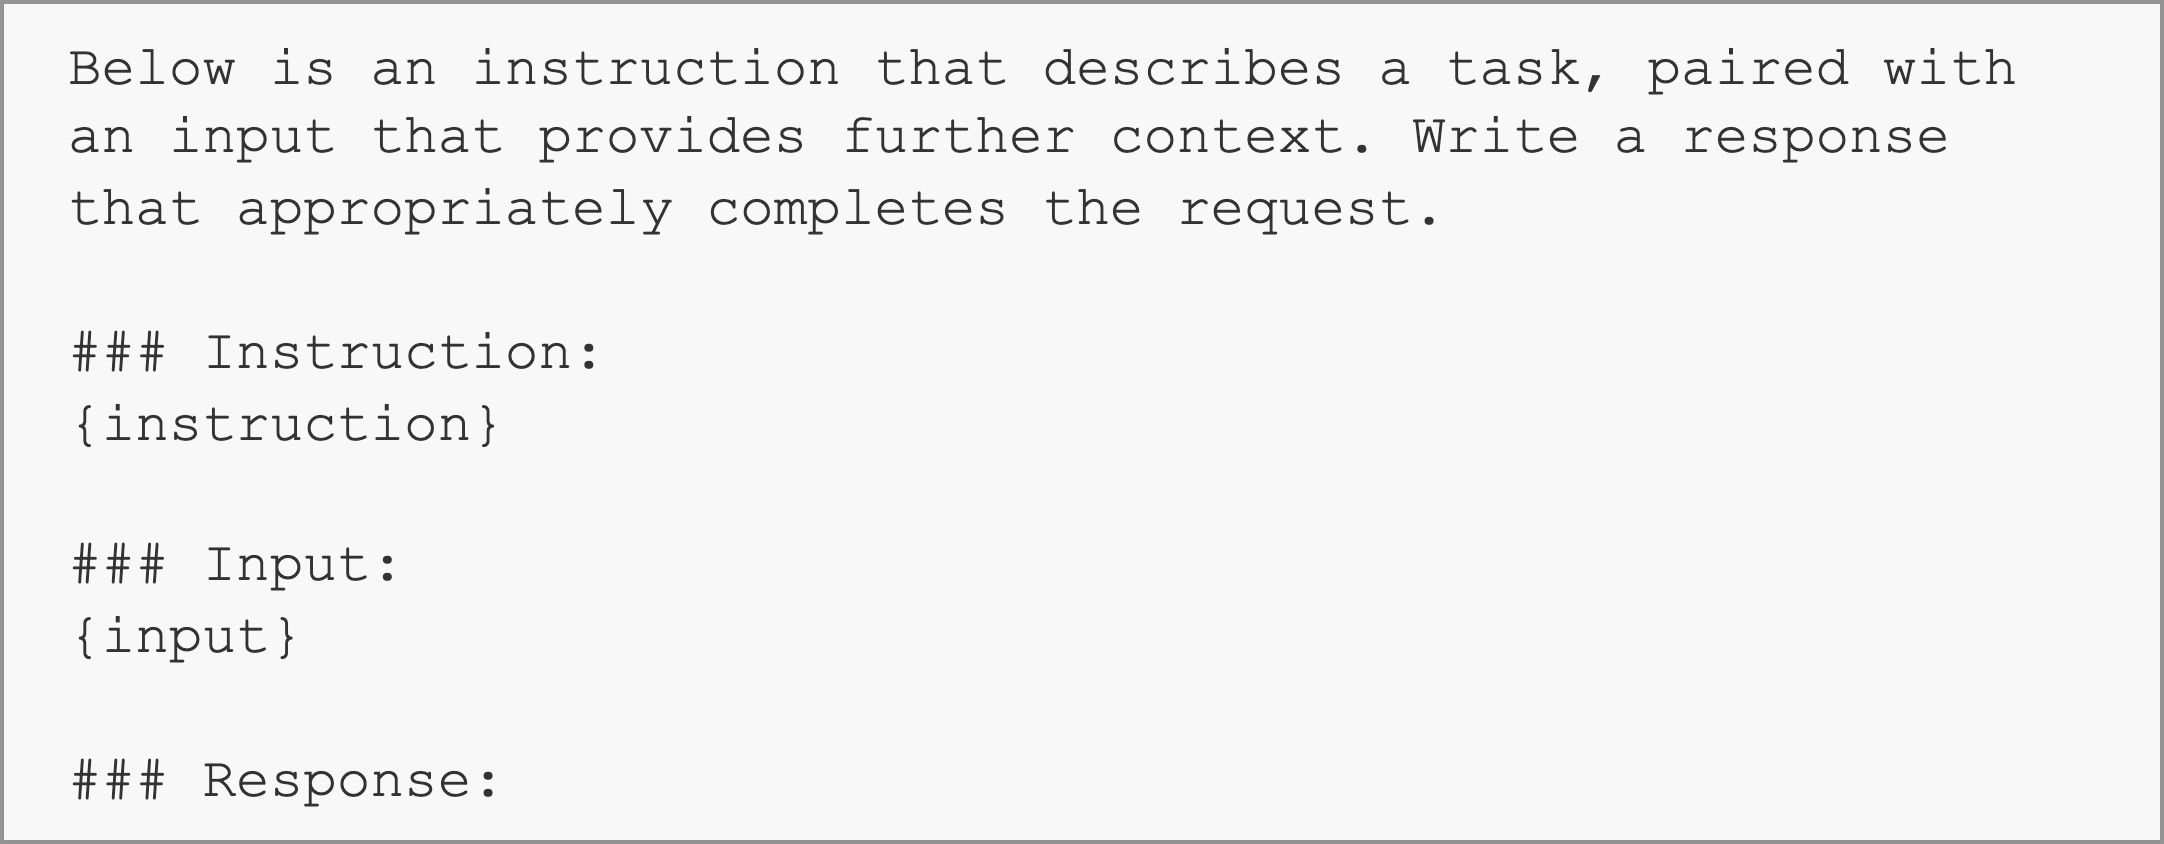
\includegraphics[width=\textwidth]{images/alpaca_prompt_format.png}}
            \caption[Overview of the original text prompt to the Stanford Alpaca model, with additional input.]{Overview of the original text prompt to the Stanford Alpaca model \cite{taoriStanfordCRFM, taoriStanfordAlpacaInstructionfollowing2023}, with additional input.}
            \label{fig:alpaca_prompt_format}
        \end{figure}

        % Modified prompt format
        \begin{figure}[htb]
            \centerline{
            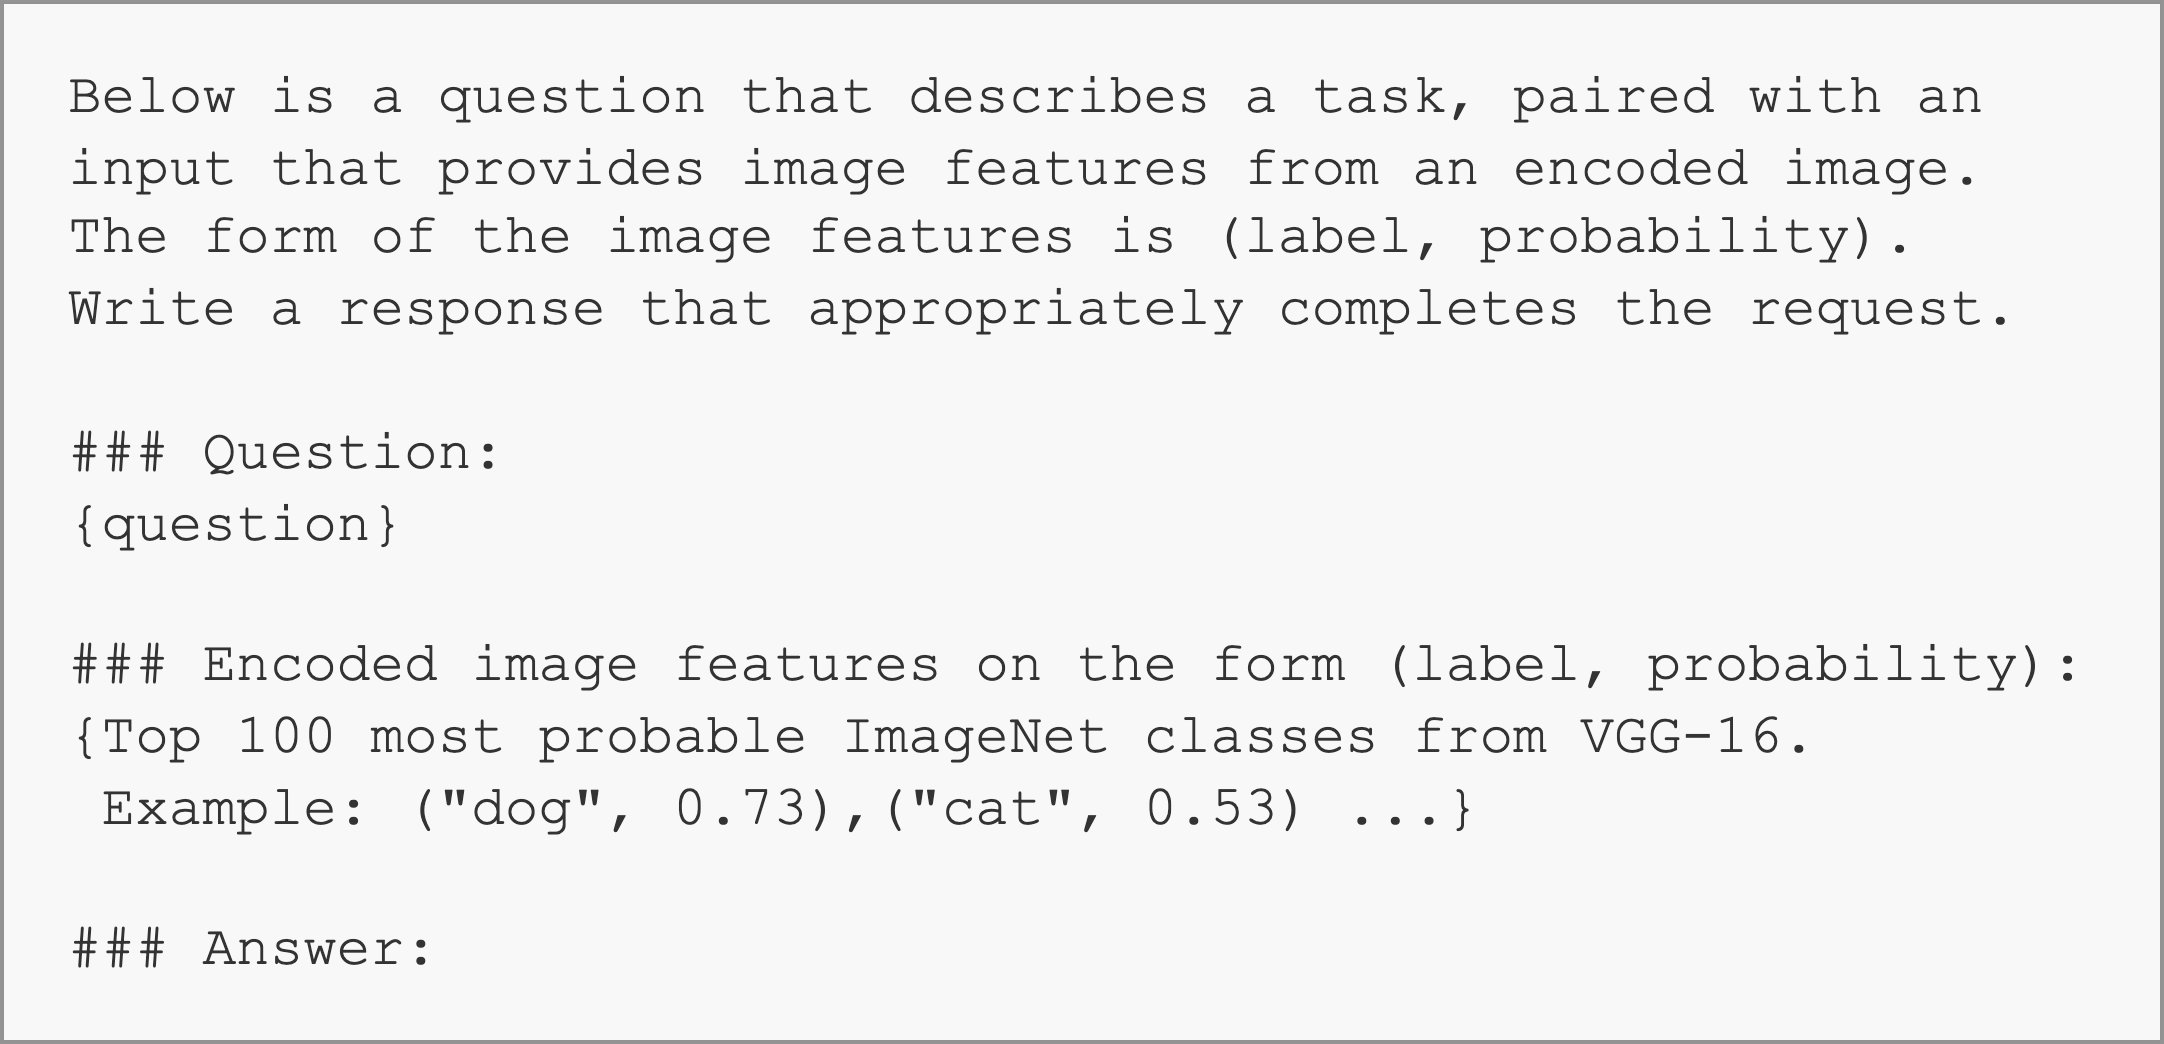
\includegraphics[width=\textwidth]{images/alpaca_modified_prompt_format.png}}
            \caption{Overview of the modified text prompt to the Alpaca-LoRA model, including extracted image features.}
            \label{fig:alpaca_modified_prompt_format}
        \end{figure}


        \subsubsection{Text encoding}
        % How to encode the text

        To break down the raw text data given in the prompt into smaller, standardized units, called tokens, a text tokenization process is needed. This assures that text models, \glspl{llm} in this case, tokenization is essential to transform unstructured text data into a format that can be processed by the model.
        
        Given that \glspl{llm} have been trained on specific tokenization schemes that use unique tokenization rules and vocabularies. If a different tokenizer is used to pre-process the text data, the tokenization output may not be compatible with the language model's vocabulary and encoding scheme, leading to poor model performance and incorrect predictions.
        
        Using the tokenizer from the language model ensures that the tokenization process is consistent with the training data and the model's internal encoding scheme. 
        
        This consistency ensures that the same tokenization scheme is used during both training and inference. This consistency is essential for the model to learn the patterns and relationships within the text data effectively. If a different tokenizer is used during inference, the output may not be the same as the input used during training, which in turn can lead to undesirable results.
        
        The tokenizer from the language model has also been trained on a large corpus of text data and optimized to handle specific language patterns and nuances. This makes it more effective than other tokenization schemes that may not have the same level of optimization and language-specific knowledge. Using the language model's tokenizer ensures that the text data is pre-processed in a way that is most compatible with the model, leading to better performance and more accurate predictions.

        The tokenizer used in this implementation is the one used by the original LLaMA model \cite{touvronLLaMAOpenEfficient2023} and the specific implementation of the used LlamaTokenizer is based on SentencePiece \cite{LLaMATokenizer, Sentencepiece}. This tokenizer and detokenizer allow for an unsupervised, end-to-end system that does not need any language-specific processing. 
        
        
        \subsection{Training the model}
        % How to train the model
        \subsubsection{Context window and cutoff length}
        \label{sec:3_cutoff}
        The context window of a language model refers to the number of words or tokens that are considered in predicting the next word or token. The context window is typically linked to both the input prompt and the output since the model refers to the input when generating the output. When training large language models, the model receives a sequence of input tokens and produces a sequence of output tokens. The context window refers to the size of the input sequence that the model uses to generate each output token. Similarly, when fine-tuning a pre-trained language model on a specific task, as in this case, the context window is also linked to both the input and the output. The input would consist of the task-specific prompt combined with the context window, and the output would be the predicted tokens that follow the input. By adjusting the size of the context window, researchers can control the amount of context that the model uses to generate its predictions, which can impact both the accuracy and the efficiency of the model.

        % how context window and cutoff length are related 
        Cutoff length is a term often used while fine-tuning a pre-trained language model for a specific task, where the model is fine-tuned on examples that consist of a prompt or query followed by a target output. The prompt cutoff length specifies the maximum length of the prompt that can be used during fine-tuning.

        The context window and cutoff length are therefore not the same, but closely related features that should be considered in conjunction with each other. In practice, the context window can therefore be seen as a way to capture longer-term dependencies between words in a sequence, while the prompt cutoff length is a constraint on the length of the input that the model is trained to handle for a specific task.
        
        

        % Specific cutoff length
        To train the model to interpret images, the updated input prompt shown in Figure \ref{fig:alpaca_modified_prompt_format} was used. The prompt cutoff length was updated from the original 256 to 1485 tokens. The original LLaMA model was trained on 2048 tokens \cite{SequenceContextLength}, and the Alpaca model is fine-tuned with 512 tokens as the cutoff length. The authors of the Alpaca-LoRA model used in this experiment analyzed the training data and found that 96\% of the prompts could be answered by using a cutoff length of 256 tokens. When deciding on the new token length, including the top 100 classes from VGG-16, the LlamaTokenizer was used to encode only the features extracted from the image. 
        
        When the class prediction score was presented using Numpy's floating number with 32 bits of precision, the average token length only for image features where 162'654. As this would be an increase of the token length of more than 63 thousand percent, it was considered an increase too large to be reasonable for the model. Because the used language model uses the LoRA technique to lower memory consumption, such a large cutoff length would technically be feasible, but regarding the increased training and inference time, it was deemed too inefficient.  
        To decrease the image token length, the prediction score was converted to floats with 16 bits of precision. In practice, this would not make a difference when fed into the language model, as the predicted class is just a placeholder for the underlying feature maps extracted. The upside of cutting the precision is that the average token length of the extracted 100 classes was cut down to 144'654 tokens. The reduced token length is an 11\% reduction of tokens, which still would benefit from a further reduction. To give a further decrease in the length of the prediction scores, they were rounded to three decimals. This will still give the language model insight into the extracted class labels and the relationship between the classes, while also giving a great reduction in prediction score token length. The resulting rounded scores have a length of 1229 tokens, resulting in a reduction of 99\% from the original 32-bit precision score. Combined with a text prompt length of 256 the total cutoff length is 1485 tokens. This cutoff length is therefore designed to cover 96\% of the original prompts, while also incorporating the 100 most probable classes and their predictions. 


         


        \subsubsection{Evaluation metrics}
        % Evaluation metrics used

        % Precision and  Recall
        \paragraph{Precision and Recall\\}
        Precision and recall are two important metrics used in classification tasks to evaluate the performance of a model. 
        Both precision and recall are based on the values in the confusion matrix, which is a table that summarizes the performance of a classification model. The confusion matrix contains four values: true positives, false positives, true negatives, and false negatives. True positives and false positives correspond to the model's positive predictions, while true negatives and false negatives correspond to the negative predictions. An example of a confusion matrix can be seen in Figure \ref{fig:confusion_matrices}. The precision and recall are defined as follows.
        

        \begin{itemize}
            \item Precision: the ratio of correct answers among all answers proposed by the model, and it measures how precise the model's positive predictions are. The precision score can be calculated as follows:
            
            \begin{equation}
                \text{Precision} = \frac{\text{True Positive}}{\text{True Positive} + \text{False Positive}}
            \end{equation}
            
            \item Recall: the ratio of correct answers proposed by the model among all possible correct answers, and it measures how well the model is able to identify positive instances. The recall score can be calculated as follows:

            \begin{equation}
                \text{Recall} = \frac{\text{True Positive}}{\text{True Positive} + \text{False Negative}}
            \end{equation}
        \end{itemize}


        \begin{figure}[htb]
         \centerline{
             \begin{subfigure}[b]{0.5\textwidth}
                 \centering
                 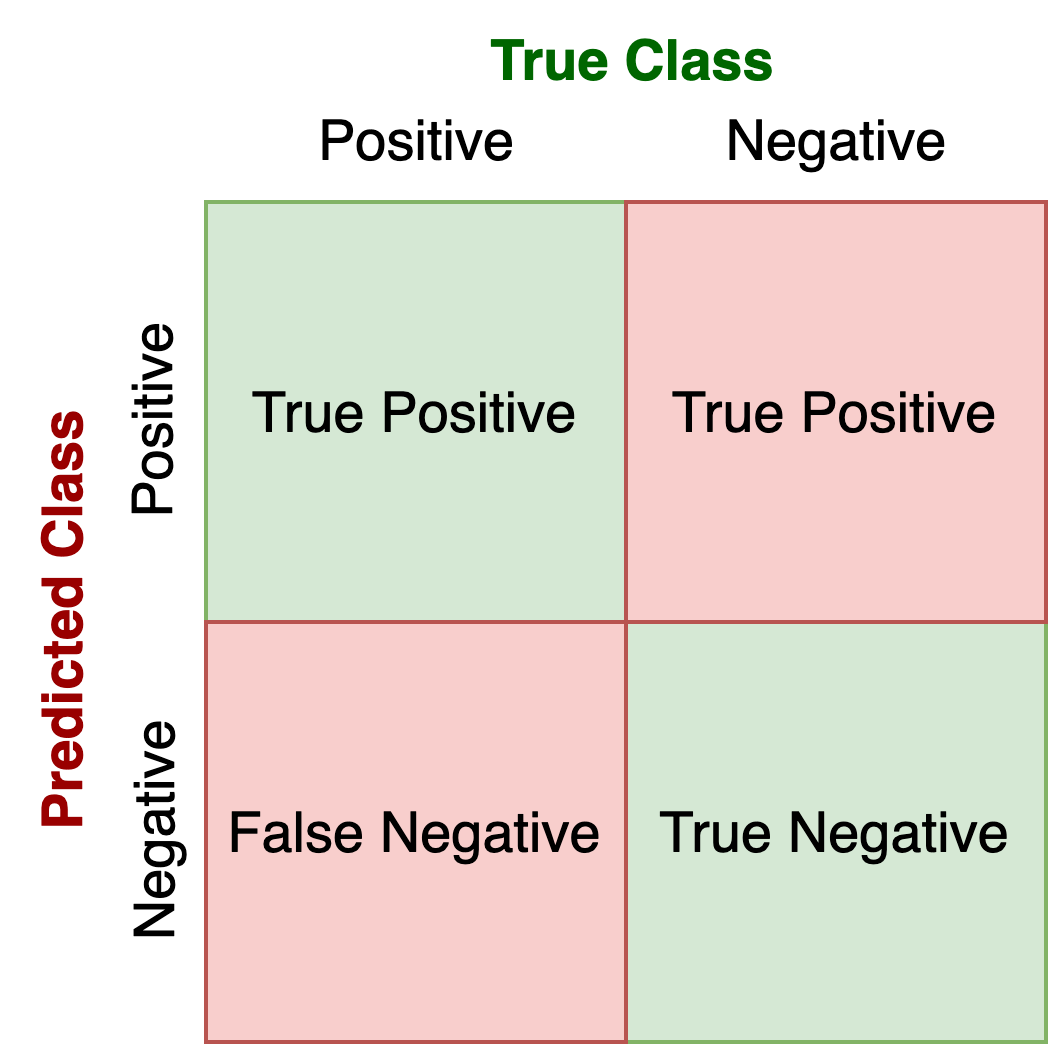
\includegraphics[width=\textwidth]{images/confusion_matrix_binary.png}
                 \caption{Example of a confusion matrix of a binary classifier. A perfect classifier would have just true predictions.}
                 \label{fig:confusion_binary}
             \end{subfigure}
             \hspace{0.1\textwidth}
             \begin{subfigure}[b]{0.5\textwidth}
                 \centering
                 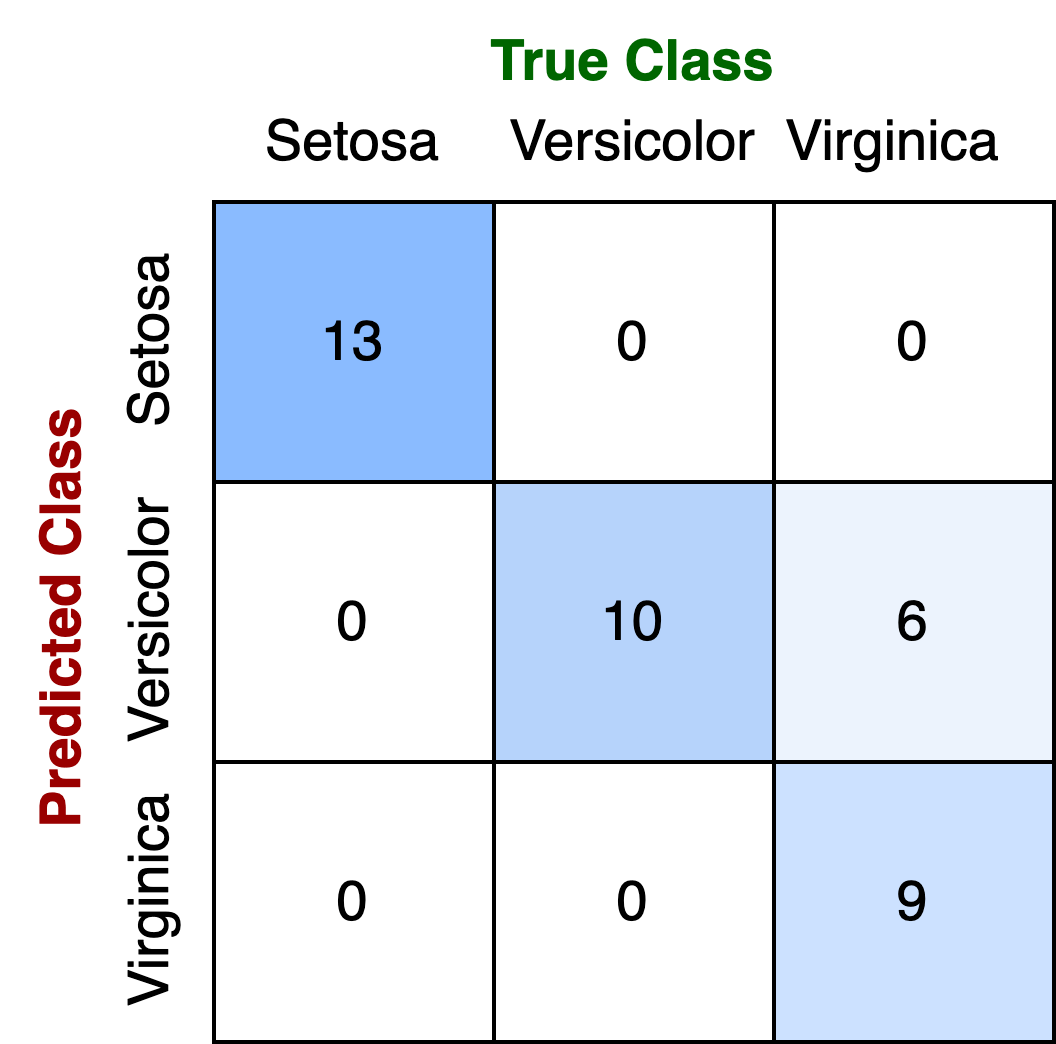
\includegraphics[width=\textwidth]{images/confusion_matrix_multi.png}
                 \caption{Example of a confusion matrix of a multi-class classifier. An adapted example from scikit-learn \cite{ConfusionMatrix}.}
                 \label{fig:confusion_multi}
             \end{subfigure}
             }
            \caption{Example of confusion matrices, both for a binary (a) and multi-class (b) classifier.}
            \label{fig:confusion_matrices}
        \end{figure}


        % Accuracy
        \paragraph{Accuracy\\}
\begin{comment}
https://www.statology.org/f1-score-vs-accuracy/
Accuracy:

Pro: Easy to interpret. If we say that a model is 90% accurate, we know that it correctly classified 90% of observations.

Con: Does not take into account how the data is distributed. For example, suppose 90% of all players do not get drafted into the NBA. If we have a model that simply predicts every player to not get drafted, the model would correctly predict the outcome for 90% of the players. This value seems high, but the model is actually unable to correctly predict any player who gets drafted.
\end{comment}
        Accuracy is a commonly used evaluation metric in statistics and artificial intelligence for classification models. It is a metric that is easy to interpret by humans because it is a measure of the percentage of correctly predicted labels out of all the predictions made by the model. Accuracy is a useful metric when the classes in the dataset are balanced, meaning that the number of instances for each class is roughly equal. However, when the classes are imbalanced, accuracy can be a misleading metric. For instance, in a dataset with 95\% of the samples belonging to class A and only 5\% belonging to class B, a model that always predicts class A will have an accuracy of 95\%, but will not be useful in practice.

        Moreover, accuracy does not account for false positives and false negatives, as seen in Formula \ref{eq:accuracy}. False positives occur when the model predicts a positive label for a sample that is negative, while false negatives occur when the model predicts a negative label for a sample that is positive. In some applications, such as medical diagnosis, false negatives may be more costly than false positives, and accuracy alone may not be an adequate metric for evaluating model performance. Therefore accuracy can be a useful and easily understandable metric when there is no critical downside predicting false negatives and the classes in the dataset are balanced. Often when dealing with real-world datasets the classes are not balanced and a more suitable metric can be the $F_1$ score.
        


        \begin{equation}
            \text{Accuracy} = \frac{\text{True Positive} + \text{True Negative}}{\text{Total Sample Size}}
            \label{eq:accuracy}
        \end{equation}


        % F1 score
        \paragraph{$\mathbf{F_1}$ score\\}

    
        The $F_1$ score is a statistical metric used to measure a model's performance on a dataset. It evaluates the performance of a binary classifier, which is a classification system, which makes predictions for two possible classes, for example, positive and negative. The $F_1$ score can be calculated using the formula in Equation \ref{eq:f1}.

        \begin{equation}
            F_1 = 2 \frac{\text{Precision} \cdot \text{Recall}}{\text{Precision} + \text{Recall}}
            \label{eq:f1}
        \end{equation}

        In the context of question answering by a large language model, the $F_1$ score can be used to evaluate the accuracy of the model's responses to questions. Specifically, the score measures the harmonic mean of the model's precision and recall.

        \begin{comment}
https://www.statology.org/f1-score-vs-accuracy/
F1 Score:

Pro: Takes into account how the data is distributed. For example, if the data is highly imbalanced (e.g. 90% of all players do not get drafted and 10% do get drafted) then F1 score will provide a better assessment of model performance.

Con: Harder to interpret. The F1 score is a blend of the precision and recall of the model, which makes it a bit harder to interpret.

As a rule of thumb:

We often use accuracy when the classes are balanced and there is no major downside to predicting false negatives.

We often use F1 score when the classes are imbalanced and there is a serious downside to predicting false negatives.
        \end{comment}
        

        % Summary
        

% SUMMARY:

\chapter{Experiments, Results, and Discussion}
\label{4_investigatory_experiments}

\begin{comment}
INTRO: What will you look at in this chapter and why? Again, point back to the summary in the last chapter, and say that here you want to experiment with and evaluate the proposed “solution”.
\end{comment}

% INTRO:
\section{Intro}
\begin{comment}
    List of the different runs that have been made.
\end{comment}


In this chapter, the Alpaca-VQA model presented in the previous chapter is tested on two different dataset sizes. First, hyperparameters, their values, and the reasons for choosing these are discussed. Then an investigatory experiment is conducted using a smaller dataset to get initial results for training on more data. 
These results are analyzed to understand better how the model responds to the data, aiding understanding how the model responds to the data.
The Alpaca-VQA model is then trained on 20,000 samples, and its results are discussed. Methods for visualizing transition scores and training a proxy model explained by \gls{lime} are implemented when the Alpaca-VQA model has finished training. 
The insights from these supplementary methods uncovered a possibility that the model did not evaluate the image features when predicting an answer. A language-only Alpaca-VQA model was tested to test this hypothesis, and its findings are discussed. 
Finally, a more general examination of the findings in this work is discussed. 


\begin{comment}
MIDDLE SECTIONS: Explain your experiments and evaluations. Include a detailed description of the data you have used, and which metrics you include. It is nice to discuss what the results also mean (in general and in the context of your problem statement), not only what you can observe. Also, try to explain WHY the results turn out as they do. You are a researcher and should try to understand why things happen, not only observe what happens.
\end{comment}

\section{Hyperparameters}
    The Alpaca-VQA model is based on the Stanford Alpaca model and therefore draws inspiration when deciding on hyperparameters from their findings.
    To finetune the Stanford Alpaca model, the authors suggest training for two or three epochs. The low number of epochs is to prevent the model from forgetting the previous knowledge and still be able to use the knowledge gathered from the original training corpus, known as \textit{catastrophic forgetting}. Therefore, for the following experiments, the hyperparameters were chosen as in \autoref{table:hyperparameters_alpaca}. 
    
    The \gls{lora} parameters were selected to be the same as the original Alpaca-LoRA implementation. 
    The transformer architecture contains four weight matrices for the self-attention module. These weights are for \textit{query} ($W_q$), \textit{key} ($W_k$), \textit{value} ($W_v$) and \textit{output} ($W_o$).
    In the paper introducing \gls{lora}, the authors find that when applying \gls{lora} to the attention weights for \glspl{llm}, specifically GPT-3 on the datasets WikiSQL \cite{zhongSeq2SQLGeneratingStructured2017} and MultiNLI \cite{williamsBroadCoverageChallengeCorpus2018}, they achieved the best results overall by only adapting the $W_q$ and $W_v$ matrices. The developer of Alpaca-LoRA also confirmed these results, and therefore the experiments in this thesis will also use these update matrices.
    The authors of \gls{lora} also did experiments for GPT-2 and GPT-3 to see which effect the rank \textit{r} would have on the performance. They found that \gls{lora} performs competitively with small values of \textit{r}, especially when only adapting $W_q$ and $W_v$.

    As seen in \autoref{table:lora_parms}, the \gls{lora} update parameters are only 0.0622\% of the original amount of trainable parameters in the Alpaca-VQA model. This low amount of trainable parameters using \gls{lora} update matrices results in considerably faster training and lower memory use.

    
    The rationale for deciding on the batch size and micro-batch size values was to make it fit in the available \gls{ram} on the \gls{gpu} it was trained on. Since the current state of the code can only utilize a single \gls{gpu}, it was necessary to fit the model on the \gls{gpu} while training. 
    The \glspl{gpu} used for this experiment was an Nvidia RTX2080Ti with 11 GB of \gls{vram} and an Nvidia A100 with 40 GB of \gls{vram}. For the initial experiment, the smaller RTX2080Ti was used not to demand more compute resources than needed. The A100 was used when training on the larger datasets, and the batch size was doubled to 256, which benefited from more \gls{vram}. The increased batch size would allow the model to see more of the samples simultaneously during training.
    The number of epochs was kept to three while the step length was increased, effectively making the model evaluate more often in each epoch.
    
    The size of the validation set was chosen to be roughly 30\% of the training data, and the cutoff length was chosen to be 1485, as this corresponds to $256 \text{ question tokens} + 1229 \text{ tokens from the encoded image}$, as discussed in Section \ref{sec:3_contex_cutoff_eval}. This token length should allow the model to see most of the available input data, both text and images when predicting the output.

    The temperature parameter influences the probabilities when predicting new tokens. In practice is a measure of how creative the language model should be during text generation. A lower temperature value makes the model choose tokens it is more confident are correct, and a larger value makes it more creative. As this task is to answer a question, the goal is more based on facts than creativity, and therefore the temperature was chosen to be 0.1.

    During generation, the Alpaca-VQA model uses beam search with four beams. This means that it generates and searches in four sequences before deciding on the sequence with the highest combined transition score. This sequence is the one that the model is most confident fulfills the task.
    The values of \textit{top-K} and \textit{top-p} influence how many words are considered in the probability distribution during token generation. A top-K of 40 means it considers the 40 most probable tokens in the distribution. Top-p narrows down this distribution of top-K words to the smallest group that fulfills a cumulative probability above the set value. 
    With these hyperparameters set during generation, the Alpaca-VQA model achieves a reasonable broad distribution of tokens to sample from while maintaining the computation demand reasonable. 
    
    If no further details are given in the experiments, the parameters described here are the ones used in the following experiments.

    \begin{table}[htb]
    \centering
    \begin{tabular}{ r r c } 
         \multicolumn{3}{c}{\textbf{Alpaca-VQA Hyperparameters}}\\
        \toprule
           \multicolumn{2}{c}{\textbf{Hyperparameter}} & \textbf{Value}\\ 
        \midrule
            \multicolumn{3}{c}{\textbf{Training}}\\
            
            \multicolumn{2}{r}{Batch size:} & 128 \\
            \multicolumn{2}{r}{Micro batch size:} & 4 \\
            \multicolumn{2}{r}{Number of epochs:}& 3 \\
            \multicolumn{2}{r}{Learning rate:} & 0.0003 \\ 
            \multicolumn{2}{r}{Validation set size:} & 30\% of training data\\
        \midrule
            \multicolumn{3}{c}{\textbf{Text Generation}}\\
            \multicolumn{2}{r}{Temperature:} & 0.1\\
             \multicolumn{2}{r}{Cutoff length:} & 1485 \\
            \multicolumn{2}{r}{Top-p:} & 0.75\\
            \multicolumn{2}{r}{Top-K:} & 40\\
            \multicolumn{2}{r}{Number of beams:} & 4\\
        \midrule
            \multicolumn{3}{c}{\textbf{LoRA}}\\
            \multicolumn{2}{r}{Rank r:} & 8 \\
            \multicolumn{2}{r}{Alpha $\alpha$:} & 16 \\
            \multicolumn{2}{r}{Dropout:} & 0.05 \\
            \multicolumn{2}{r}{Weight Matrices:} & $W_q$, $W_v$ \\[0.5ex]
        \bottomrule
    \end{tabular}
    \caption{Hyperparmaters selected for the initial experiment with Alpaca-VQA, fine-tuning the LoRA matrices on the ImageCLEFmed-MEDVQA-GI-2023 dataset.}
    \label{table:hyperparameters_alpaca}
    \end{table}

    \begin{table}[htb]
    \centering
    \begin{tabular}{ r c } 
        \multicolumn{2}{c}{\textbf{LoRA Training Parameters}}\\
        \toprule
             %[0.5ex] 
           Parameter & Value \\
        \midrule
            Number of trainable LoRA parameters: & 4,194,304\\
            All parameters in Alpaca-VQA: & 6,742,609,920\\
            Trainable percent: & 0.0622\%\\[0.5ex]
        \bottomrule
    \end{tabular}
    \caption{Overview of the number of trained parameters using LoRA.}
    \label{table:lora_parms}
    \end{table}

    In the next section, an investigatory experiment will be carried out. By testing the model on a smaller dataset, it can be explored how the model responds to the dataset without using extensive computational resources. The results from this experiment will be analyzed and help make the final model a better fit for the task. 


\section{Investigatory Experiment}

Before training the model on the complete dataset, a subsection of the available training data was used to see how the model would respond. Running the model on smaller training data makes it possible to get initial results quickly, providing insight into where the method could be improved. 

    \subsection{Training: 5000 samples}

    The investigatory experiment was conducted using a subset of the original \textit{ImageCLEFmed-MEDVQA-GI-2023} dataset. The subset was chosen to be on 5000 samples, corresponding to 9,7\% of the total dataset. The reason for doing the initial investigatory experiment with this subset is to test the feasibility of the method and implementation without using excessive time and computing resources. 
    
    

    \subsubsection{Results}


    The graph in \autoref{fig:MED-QA-ImageID_5000_samples-Training_loss} shows the training and evaluation loss for the training session over 3 epochs, with 8 evaluation steps during training. As seen by the graph, the model has a decrease in loss midway before it flattens out without a further significant decrease. This can suggest that the model is able to fit the data in the training set. However, since it does not continue to decrease, it indicates that the model has already learned the relevant parts midway through the training. It can also be seen that the evaluation loss follows the training loss closely, indicating that the model does not overfit the available data. The loss flattens towards the end, suggesting that the chosen hyperparameters were reasonable for the size of this training data. 
    However, changing hyperparameters such as learning rate or \gls{lora} parameters may improve the model. By increasing the size of the \gls{lora} update matrices, the model could learn more features, which could increase the fit.

    It can also be seen that evaluation loss closely follows the same trend as the training loss. The loss on the validation data is expected to be lower than the training data, which is often called the "generalization gap". When the training and evaluation loss follow each other, separated by the generalization gap, it can indicate that the model did not overfit the available data. If the model were to overfit, the gap between training and evaluation loss would tend to increase at the end. Training loss would continue to decrease, and evaluation loss would flatten out or possibly increase. 
    
    
    \begin{figure}[htb]
        \centering
        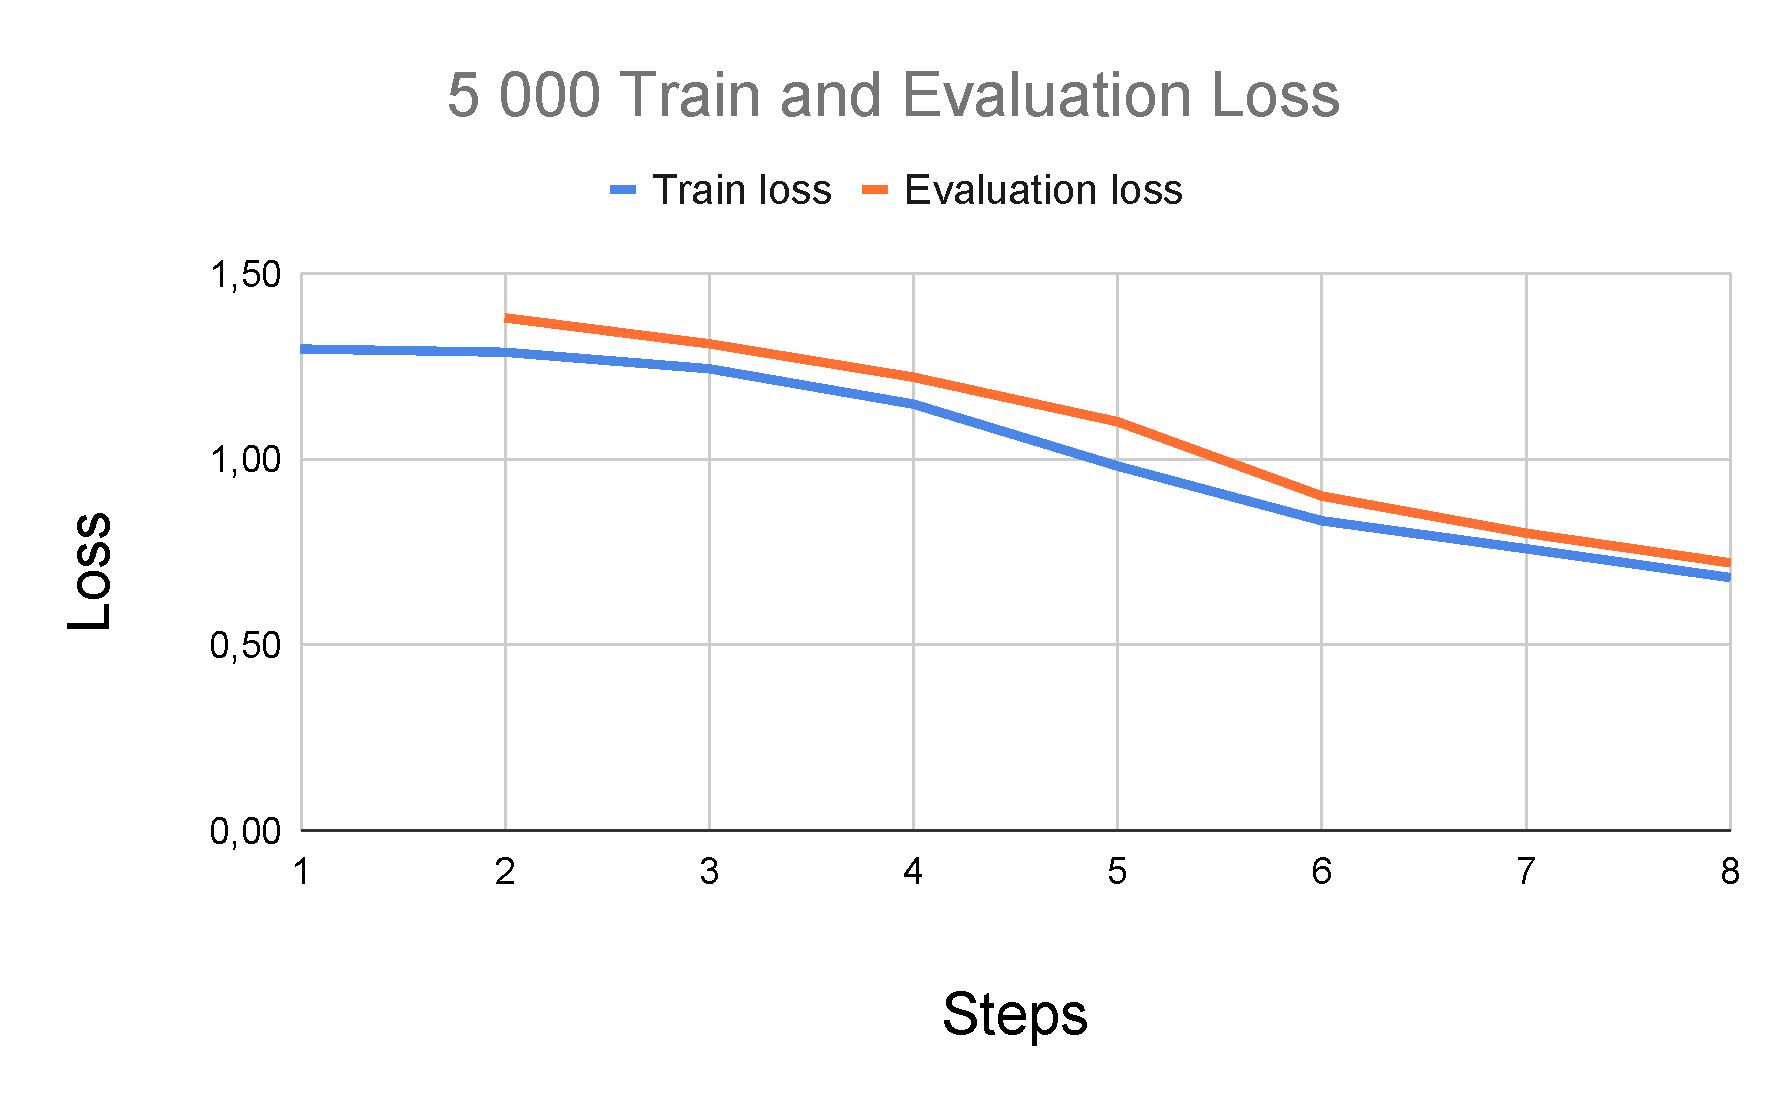
\includegraphics[width=\linewidth]{images/MED-QA-ImageID_5000_samples-Training_loss}
        \caption{Graph over training loss for the initial experiment on 5000 samples.}
        \label{fig:MED-QA-ImageID_5000_samples-Training_loss}
    \end{figure} 


    \subsubsection{Analysis}
    
    It is helpful to analyze the dataset used in training to investigate why the model often answers with "Not relevant".
    As seen in \autoref{fig:ImageCLEFmed-MEDVQA-GI-2023_answer_label_balance}, the majority of correct answers in the dataset is "Not relevant". This dataset can be balanced by either over-sample the non-majority classes or under-sample the abundant class, making the model learn that "Not Relevant" is not the best answer in 21,7\% of all questions.
    Going further in the following experiments, the original dataset will be modified. The class "Not relevant" is removed, and the rest of the dataset stays the same. The rationale behind not doing any additional sampling modifications is to reflect the natural occurrences of question-answer pairs in the original dataset. Since this dataset is based on real-world examinations in a hospital, the number of occurrences in the dataset could reflect the real-world occurrence of these findings. In contrast, if this dataset were made synthetically and did not have biases from real-world examinations, there would be more reasonable to modify the number of occurrences of the classes to get a better fit. 
    
    The Alpaca-VQA model will be trained on a larger dataset in the next section. 
    This is to explore how well it can fit the available data and which insights can be gained.


    \begin{figure}[htb]
        \centerline{
        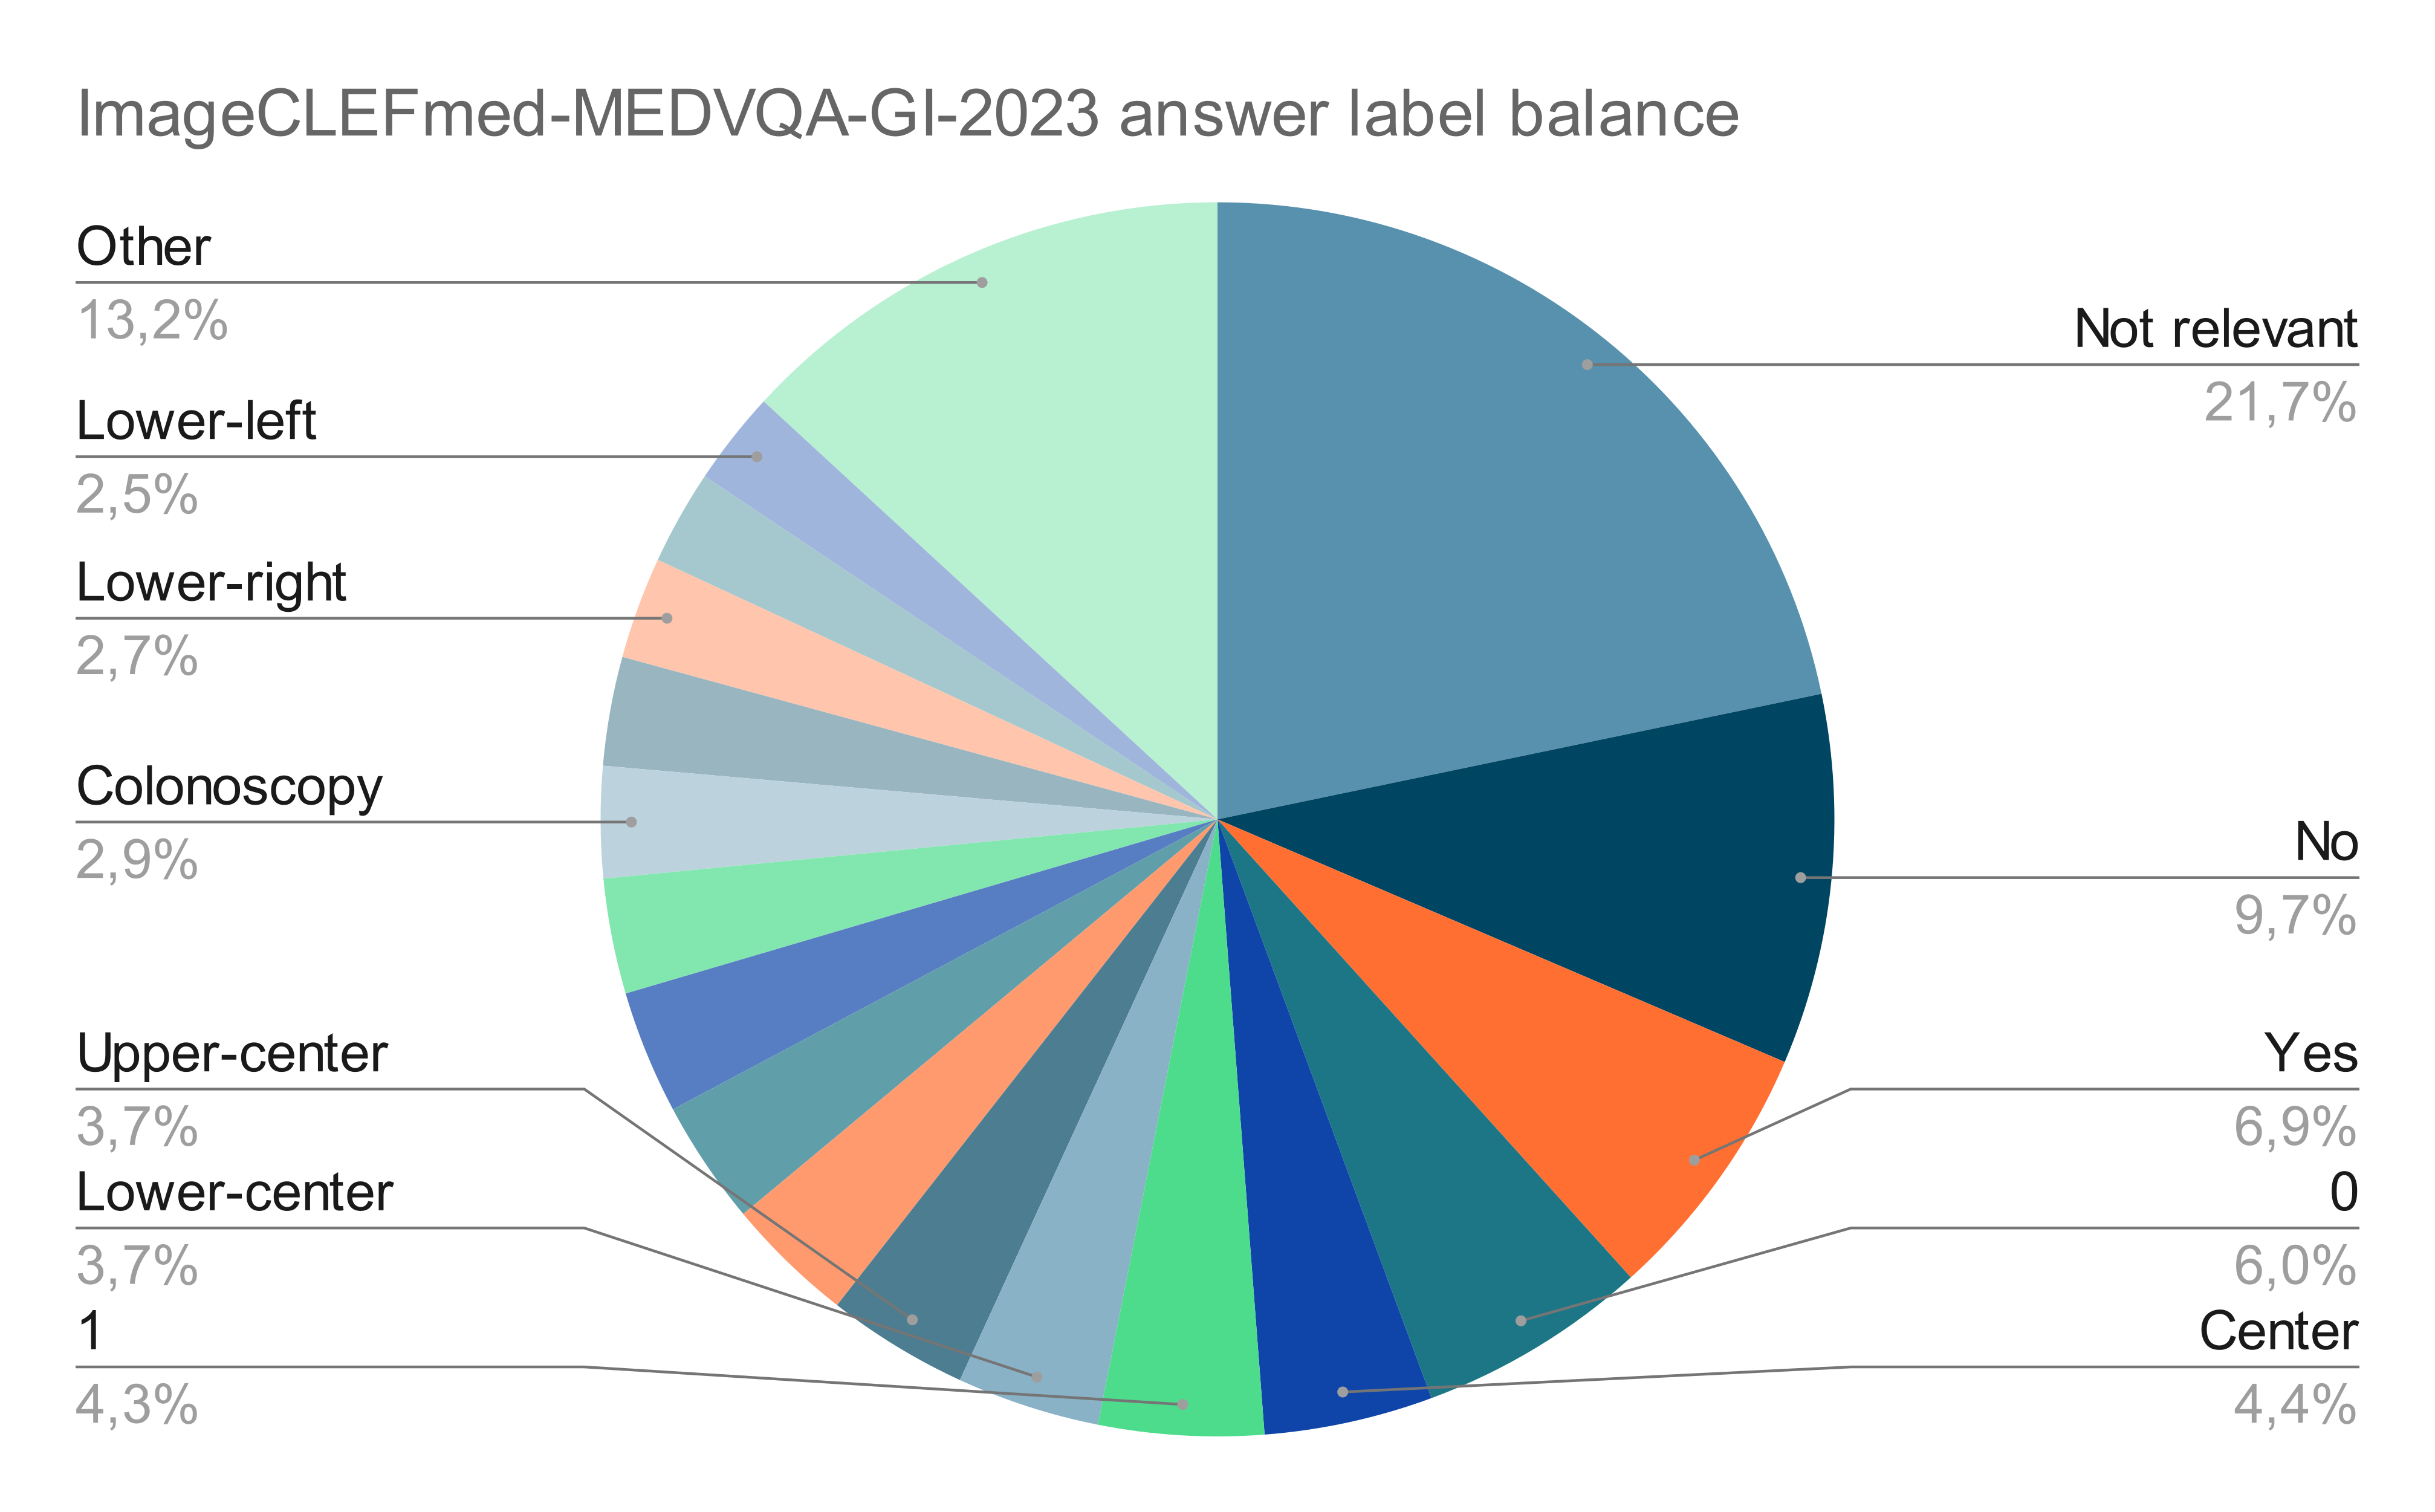
\includegraphics[width=1.08\textwidth]{images/ImageCLEFmed-MEDVQA-GI-2023_answer_label_balance}}
        \caption{Overview of the answer label balance in the ImageCLEFmed-MEDVQA-GI-2023 dataset. 
        %Note that the category "segmentation" is already removed from the dataset due to not being relevant for this task at this stage. 
        The category "Other" is a collection of 46 labels that occur in less than 2,5\% of the samples.}
        \label{fig:ImageCLEFmed-MEDVQA-GI-2023_answer_label_balance}
    \end{figure} 


    \section{Training: 20,000 samples}

    In this experiment, the model is trained on four times as much data as in the investigatory experiment. 
    As noted in the analysis of the previous experiment, the dataset used in this experiment is the same as the original, only with the class "Not relevant" removed.
    Removing this class completely also allows the model to see more relevant data since many of the chosen samples are no longer from the "Not relevant" class. 
    By removing this class, the 20,000 samples will contain more question-answer samples that are relevant to this classification problem. 
    
    The dataset was split as shown in \autoref{fig:dataset_split}, with the original dataset split in two, where the first part was used to train the model, and the second part was used to test and train the proxy model. The reason for leaving half of the dataset unused during the training of the model was to preserve unseen data that could be used to train the proxy model and to test how the model would perform on unseen data. While the model presumably would be able to fit the new task of seeing images given more data, it will still be possible to evaluate if this method is able to interpret image data. How the preserved test data is used to train the proxy model will be discussed later in \autoref{sec4:proxy_lime}.


    \begin{figure}[htb]
        \centerline{
        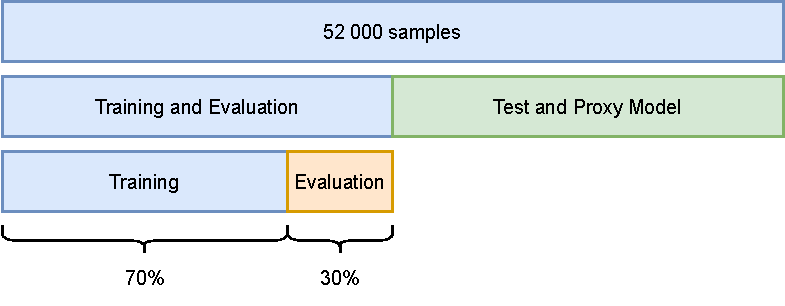
\includegraphics[width=\textwidth]{images/datatset_split.pdf}}
        \caption{Illustration on how the dataset was split into training, evaluation, and testing data.}
        \label{fig:dataset_split}
    \end{figure} 
    
    While training the model on considerably more data would be interesting, the time and computing cost for this experiment would not justify the possible better-trained system, resulting in a more generalized and nuanced model. The experiments carried out with the Alpaca-VQA model aim to investigate how an \gls{llm} would perform on a \gls{vqa} task with image features encoded in the text.
    The final dataset used for training in this experiment contains 20,000 samples, and the class distribution can be seen in \autoref{fig:ImageCLEFmed-MEDVQA-GI-2023_answer_label_balance-modified}.


    The hyperparameters used in this experiment are the same as in the previous experiment and can be seen in \autoref{table:hyperparameters_alpaca}, with a batch size of 256 as previously discussed. While the dataset used in this experiment contains four times more samples than in the previous experiment, the image feature extraction is still the extracted top 100 features from the VGG16 model. 
    Due to the similarities in the data samples, the hyperparameters are kept the same to see how the Alpaca-VQA model responds to a larger dataset.
    
    
    \begin{figure}[htb]
        \centerline{
        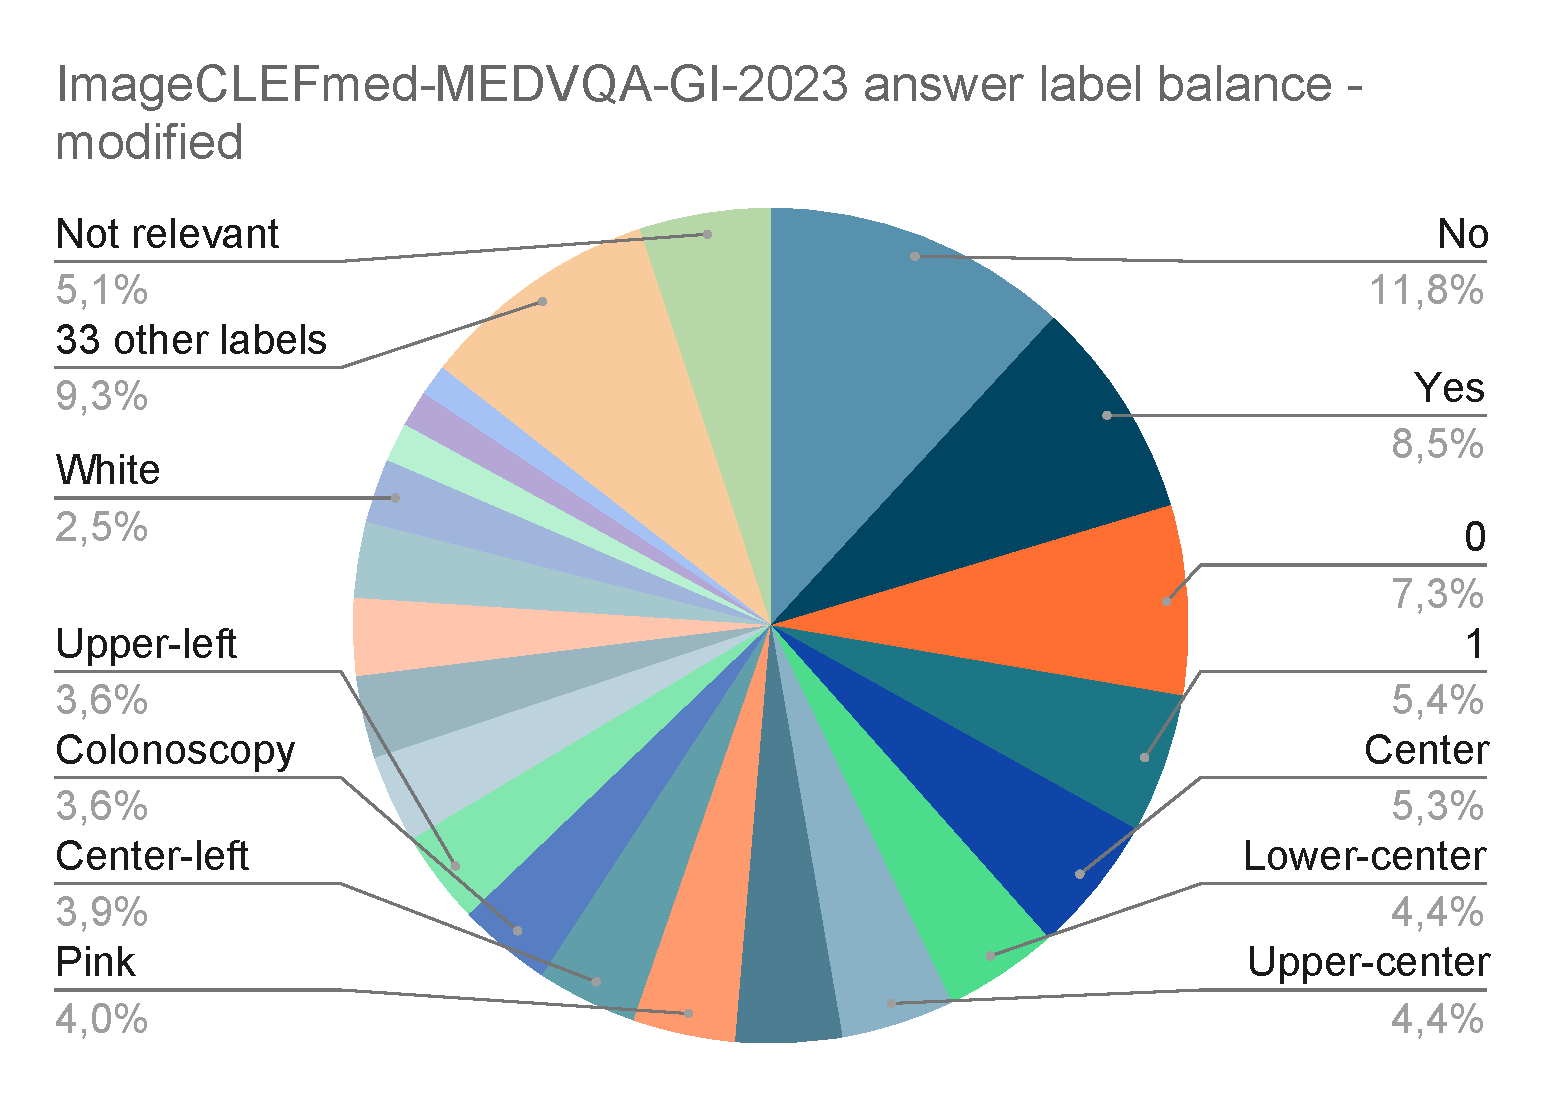
\includegraphics[width=1.08\textwidth]{images/ImageCLEFmed-MEDVQA-GI-2023-answer-label-balance-modified.pdf}}
        \caption{Overview of the answer label distribution in the ImageCLEFmed-MEDVQA-GI-2023 dataset, modified with the class "Not relevant" removed. The category "Other" is a collection of 33 smaller labels in the training data and is only used in this visualization, and is not an actual class.}
        \label{fig:ImageCLEFmed-MEDVQA-GI-2023_answer_label_balance-modified}
    \end{figure} 

    Because of the larger dataset, more evaluation steps were used to help the model correct during training. In the investigatory experiment, 8 steps were used during the runtime. In this training session, with four times as much training data, the number of steps was chosen to be every 10\textsuperscript{th} training step, resulting in 46 evaluation steps in total. 

    \begin{figure}[htb]
        \centerline{
        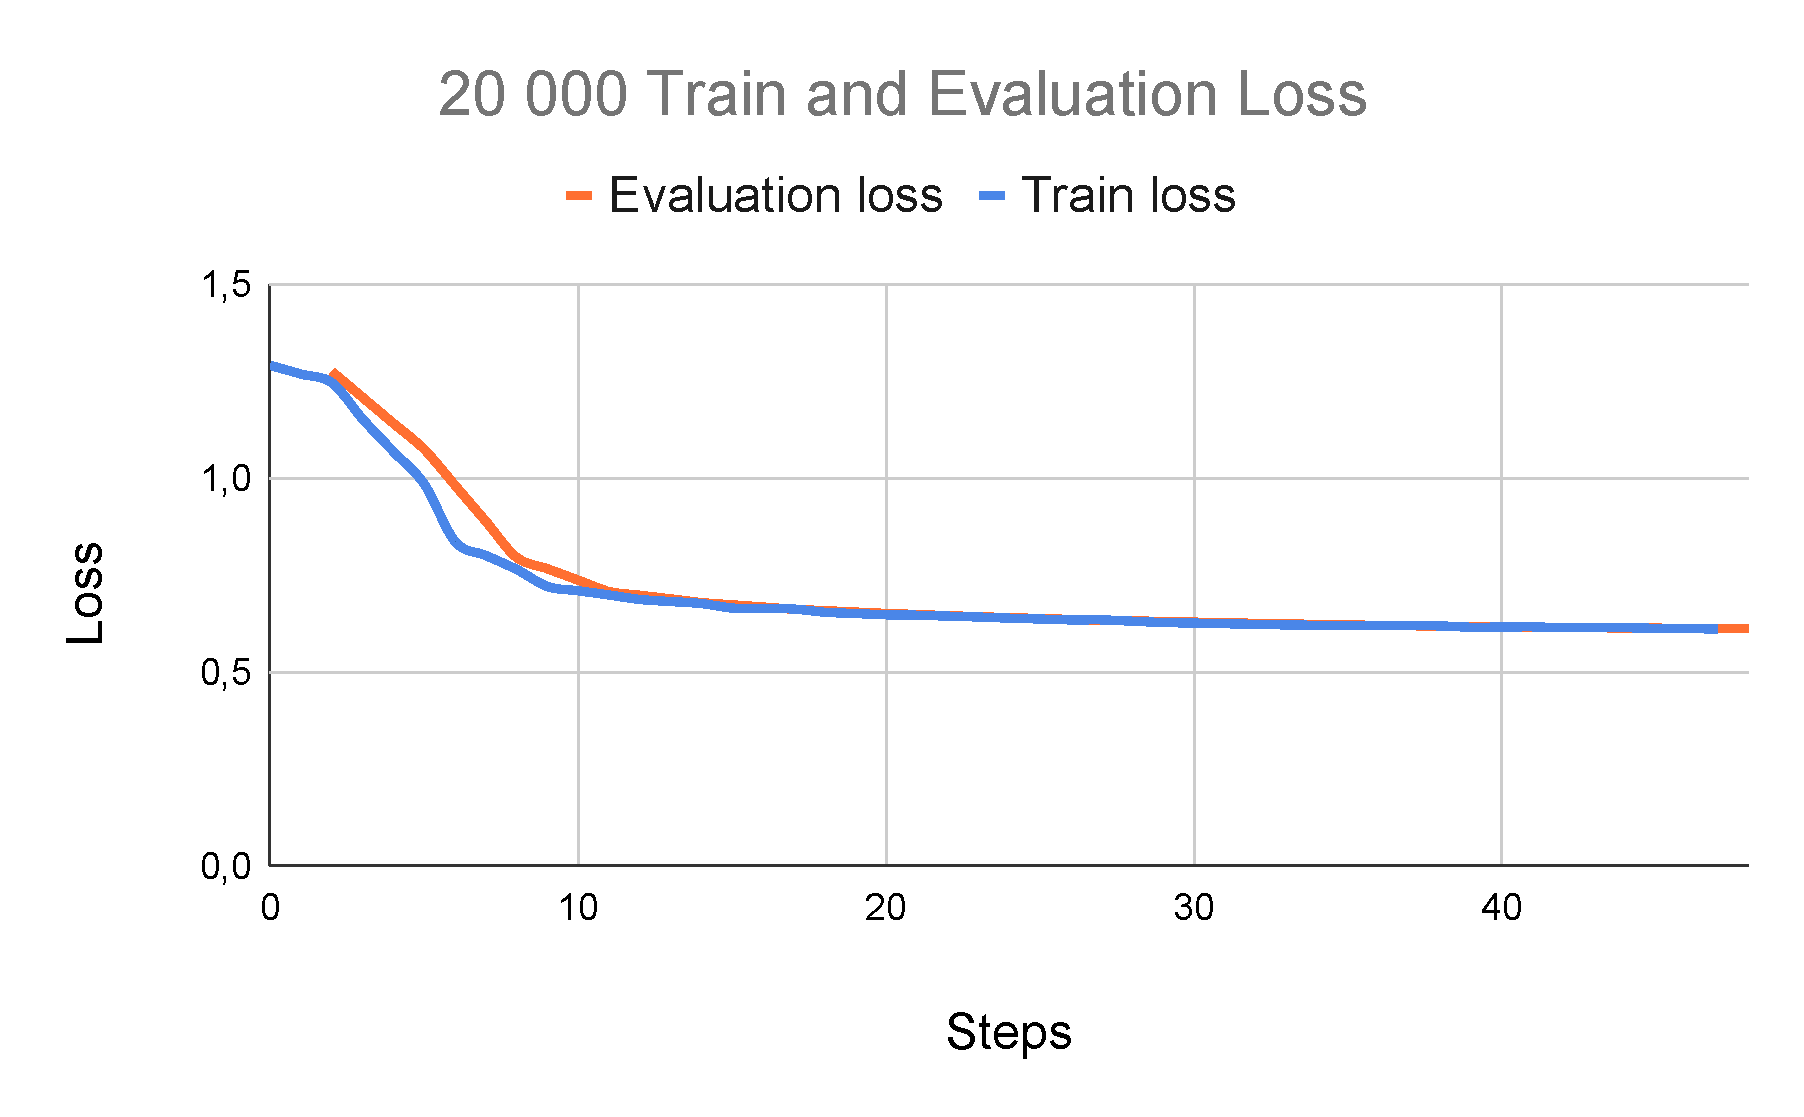
\includegraphics[width=1.07\textwidth]{images/20k_train_evaluation_loss}}
        \caption{Graph over training loss for 20,000 samples.}
        \label{fig:20k_train_eval_loss}
    \end{figure} 
    
    The Alpaca-VQA model on 20,000 samples was trained on an Nvidia A100 with 40 GB \gls{vram}. It took fifteen and a half hours to run, including image encoding, fine-tuning, and evaluating the model. 



    \section{Results}
    \label{sec4:results}
    This section evaluates the results for the Alpaca-VQA model trained on 20,000 samples, where 70\% was used as training data and 30\% as evaluation. The training results will be discussed alongside the classification report, transition scores, proxy model, and a blinded model.
    
    First, the training and evaluation loss graph during this training session can be seen in \autoref{fig:20k_train_eval_loss}. In this graph, it can be seen that the model converges relatively fast and stabilizes during the training run. This can indicate that the model was able to fit the available training data and fine-tune its \gls{lora} update matrices to the training data. Regarding the number of evaluation steps, it can be seen that the evaluation loss is approximately the same as the training loss at step 10. At this step, it can also be seen that the loss for both training and evaluation flattens out. This can indicate that the model has fitted its parameters to the available data and did not have more quality data to learn from. 


    \subsection{Classification Report}
        In order to test how the model was able to fit the training data, a test set was used. The test set was from the same dataset as the training data but naturally did not overlap with the training and evaluation data. 

        As the test result should be used later in order to fit a proxy model, the test set was chosen to be 20,000 samples. These samples should not be confused with the ones used for training and evaluation, as the dataset was split, as previously shown in \autoref{fig:dataset_split}.

        The classification report is shown in \autoref{tab:classification_report_20}. The columns are class labels, the precision, recall, and $F_1$ scores for each class, and the number of occurrences of each class in the test set in the column "Support". At the bottom of the table, the accuracy and average score are calculated. As noted in this table, the Alpaca-VQA scores an accuracy of 29\% on the test set. The number of occurrences in each class shows that this test set is also unbalanced and has approximately the same distribution as the training set.
        
        A simplified table can be found given that \autoref{tab:classification_report_20} is a large table that can be hard to interpret.
        As the $F_1$ score is a harmonic mean of the precision and recall, it can be used to indicate how well the model performs in each class. By removing the classes where the $F_1$ score is 0 from \autoref{tab:classification_report_20}, the result is a simplified representation that can be seen in \autoref{tab:classification_report_20_simpl}.
        From this table, it can be more clearly seen that the classes the trained model performs well on have a high presence in the training set, as previously shown in \autoref{fig:ImageCLEFmed-MEDVQA-GI-2023_answer_label_balance-modified}. Logically, the model performs better on data it has seen and not as well on data it has not been exposed to. From the difference between the full \autoref{tab:classification_report_20} and the simplified \autoref{tab:classification_report_20_simpl}, it can also be seen that despite having relatively high occurrence in both training and testing sets, the Alpaca-VQA model falsely categorizes classes with localization and color labels.
        One possible explanation for this is that the image encoder, the VGG16 model, does not have localization abilities, as it is not designed to output \gls{roi} or multiple objects with bounding boxes. As it is not fine-tuned on the images in this dataset but rather pretrained on ImageNet, the predicted classes may not correlate with colors.
        \begin{center}
\begin{longtable}{|c|c|c|c|c|}
\caption{Classification Report on Test Set - Model trained on 20'000 question-answer pairs.} \label{tab:classification_report_20} \\

\hline \multicolumn{1}{|c|}{\textbf{Class}} & \multicolumn{1}{c|}{\textbf{Precision}} & \multicolumn{1}{c|}{\textbf{Recall}} & \multicolumn{1}{c|}{\textbf{F1-score}} & \multicolumn{1}{c|}{\textbf{Support}}\\ \hline 
\endfirsthead

\multicolumn{3}{c}%
{{\bfseries \tablename\ \thetable{} -- continued from previous page}} \\
\hline \multicolumn{1}{|c|}{\textbf{Class}} & \multicolumn{1}{c|}{\textbf{Precision}} & \multicolumn{1}{c|}{\textbf{Recall}} & \multicolumn{1}{c|}{\textbf{F1-score}} & \multicolumn{1}{c|}{\textbf{Support}}\\ \hline 
\endhead

\hline \multicolumn{5}{|r|}{{Continued on next page}} \\ \hline
\endfoot

\hline \hline
\endlastfoot




0 & 0.54 & 0.92 & 0.68 & 1551 \\
1 & 0.52 & 0.16 & 0.25 & 1132 \\
11-20mm & 0.00 & 0.00 & 0.00 & 97 \\
2 & 0.00 & 0.00 & 0.00 & 306 \\
3 & 0.00 & 0.00 & 0.00 & 13 \\
4 & 0.00 & 0.00 & 0.00 & 2 \\
5 & 0.00 & 0.00 & 0.00 & 2 \\
5-10mm & 0.00 & 0.00 & 0.00 & 100 \\
< 5mm & 0.00 & 0.00 & 0.00 & 55 \\
>20mm & 0.00 & 0.00 & 0.00 & 71 \\
Biopsy forceps & 0.00 & 0.00 & 0.00 & 43 \\
Black & 0.00 & 0.00 & 0.00 & 9 \\
Blue & 0.00 & 0.00 & 0.00 & 4 \\
Brown & 0.00 & 0.00 & 0.00 & 10 \\
Cecum & 0.00 & 0.00 & 0.00 & 33 \\
Center & 0.00 & 0.00 & 0.00 & 1121 \\
Center-left & 0.10 & 0.14 & 0.12 & 831 \\
Center-right & 0.11 & 0.43 & 0.17 & 861 \\
Colonoscopy & 0.98 & 0.05 & 0.10 & 761 \\
Gastroscopy & 0.00 & 0.00 & 0.00 & 242 \\
Green & 0.00 & 0.00 & 0.00 & 3 \\
Grey & 0.00 & 0.00 & 0.00 & 16 \\
Ileum & 0.00 & 0.00 & 0.00 & 2 \\
Injection needle & 0.00 & 0.00 & 0.00 & 1 \\
Lower-center & 0.00 & 0.00 & 0.00 & 938 \\
Lower-left & 0.00 & 0.00 & 0.00 & 616 \\
Lower-right & 0.11 & 0.06 & 0.08 & 769 \\
Metal clip & 0.00 & 0.00 & 0.00 & 11 \\
No & 0.66 & 0.46 & 0.54 & 2505 \\
Oesophagitis & 1.00 & 0.00 & 0.01 & 240 \\
Orange & 0.00 & 0.00 & 0.00 & 16 \\
Pale Pink & 0.00 & 0.00 & 0.00 & 1 \\
Paris iia & 0.00 & 0.00 & 0.00 & 95 \\
Paris ip & 0.00 & 0.00 & 0.00 & 101 \\
Paris is & 0.00 & 0.00 & 0.00 & 125 \\
Pink & 0.38 & 0.04 & 0.07 & 819 \\
Polyp & 0.25 & 0.96 & 0.39 & 311 \\
Polyp snare & 0.00 & 0.00 & 0.00 & 30 \\
Purple & 0.00 & 0.00 & 0.00 & 1 \\
Pylorus & 0.00 & 0.00 & 0.00 & 1 \\
Red & 0.29 & 0.27 & 0.28 & 629 \\
Tube & 0.00 & 0.00 & 0.00 & 218 \\
Ulcerative colitis & 0.00 & 0.00 & 0.00 & 250 \\
Upper-center & 0.00 & 0.00 & 0.00 & 944 \\
Upper-left & 0.00 & 0.00 & 0.00 & 764 \\
Upper-right & 0.11 & 0.38 & 0.16 & 729 \\
White & 0.00 & 0.00 & 0.00 & 520 \\
Yellow & 0.02 & 0.06 & 0.03 & 79 \\
Yes & 0.59 & 0.98 & 0.74 & 1778 \\
Z-line & 0.00 & 0.00 & 0.00 & 220 \\
Brown & 0.00 & 0.00 & 0.00 & 4 \\
Grey & 0.00 & 0.00 & 0.00 & 7 \\
Purple & 0.00 & 0.00 & 0.00 & 3 \\
\hline
Accuracy &  &  & 0.29 & 20000 \\
Macro average & 0.09 & 0.08 & 0.06 & 20000 \\
Weighted average & 0.30 & 0.29 & 0.24 & 20000 \\

\end{longtable}
\end{center}
        \begin{center}
\begin{longtable}{|c|c|c|c|c|}
\caption{Simplified Classification Report on Test Set, only non-zero $F_1$ scores - Model trained on 20,000 question-answer pairs.} \label{tab:classification_report_20_simpl} \\

\hline \multicolumn{1}{|c|}{\textbf{Class}} & \multicolumn{1}{c|}{\textbf{Precision}} & \multicolumn{1}{c|}{\textbf{Recall}} & \multicolumn{1}{c|}{\textbf{F1-score}} & \multicolumn{1}{c|}{\textbf{Support}}\\ \hline 
\endfirsthead

\multicolumn{3}{c}%
{{\bfseries \tablename\ \thetable{} -- continued from previous page}} \\
\hline \multicolumn{1}{|c|}{\textbf{Class}} & \multicolumn{1}{c|}{\textbf{Precision}} & \multicolumn{1}{c|}{\textbf{Recall}} & \multicolumn{1}{c|}{\textbf{F1-score}} & \multicolumn{1}{c|}{\textbf{Support}}\\ \hline 
\endhead

\hline \multicolumn{5}{|r|}{{Continued on next page}} \\ \hline
\endfoot

\hline \hline
\endlastfoot

0 & 0.54 & 0.92 & 0.68 & 1551 \\
1 & 0.52 & 0.16 & 0.25 & 1132 \\
Center-left & 0.10 & 0.14 & 0.12 & 831 \\
Center-right & 0.11 & 0.43 & 0.17 & 861 \\
Colonoscopy & 0.98 & 0.05 & 0.10 & 761 \\
No & 0.66 & 0.46 & 0.54 & 2505 \\
Oesophagitis & 1.00 & 0.00 & 0.01 & 240 \\
Pink & 0.38 & 0.04 & 0.07 & 819 \\
Polyp & 0.25 & 0.96 & 0.39 & 311 \\
Red & 0.29 & 0.27 & 0.28 & 629 \\
Upper-right & 0.11 & 0.38 & 0.16 & 729 \\
Yellow & 0.02 & 0.06 & 0.03 & 79 \\
Yes & 0.59 & 0.98 & 0.74 & 1778 \\

\end{longtable}
\end{center}

        The classification reports are just a score on the top-level prediction of the model and do not give insight into why or how the model classifies labels. The next two subsections present different approaches to gaining insight into how the model predicts its answers. Having ways to present how the model works can aid in determining how much a user can trust the answers given by a system. 
    
    
    \subsection{Visualizing Transition Scores}
    \label{sec4:vis_transtion_scores}

    \begin{comment}
        Furthermore, analyzing the transition scores can help identify cases of hallucination or incorrect reasoning in the model's responses. If the model assigns high attention weights to irrelevant or incorrect parts of the input, it may indicate that it generates answers based on incorrect or unrelated information.
    \end{comment}
   
    This subsection explores the transition scores given by the Alpaca-VQA model when it generates its answers. These scores can provide valuable insights into how the model processes and generates its responses. This insight can help understand which words or tokens in the input are most influential when generating an answer. 
    Transition scores represent the attention or importance given to the different parts of the input sequence when generating new tokens in the output. Visualizing the transition scores can also reveal patterns and biases in the model's attention mechanism, like if the attention biases specific tokens.
    
    As the Alpaca-VQA model uses the transformer architecture from HuggingFace, implementing the transition scores is as simple as \autoref{code:transition_scores}

\begin{lstlisting}[language=Python, caption=Example of how to generate transition scores, label={code:transition_scores}]
# Generate output tokens
generation_output = model.generate(
    input_ids=input_ids,
    generation_config=generation_config,
    return_dict_in_generate=True,
    output_scores=True,
    max_new_tokens=256,
    temperature=0.1,
    top_p=0.75,
    top_k=40,
    num_beams=4,
)

# Compute transition scores
transition_scores = model.compute_transition_scores(
    generation_output.sequences, 
    generation_output.scores, 
    normalize_logits=True
)
\end{lstlisting}

    \begin{table}[htb]
        \small
        \centering
        \begin{tabularx}{\textwidth}{ @{} m{4cm}  M{3cm}  Y  Y @{} }
            \multicolumn{4}{c}{\textbf{Transition Scores}}\\ 
            \toprule 
            Question & Ground Truth & Predicted Token & Transition Score \\
            \midrule
            
            Are there any anatomical landmarks in the image? & No & No & 21.20\%\\
        \noalign{\vskip 2mm} 
        \cline{1-4}
        \noalign{\vskip 2mm}    
        
          \multirow{3}{=}{Where in the image is the instrument?} & \multirow{3}{*}{Upper-left} & Lower & 50.49\% \\
             &  & - & 99.76\%\\ 
             &  & left & 40.16\% \\
        \noalign{\vskip 2mm} 
        \cline{1-4}
        \noalign{\vskip 2mm}    
          How many polyps are in the image? & 0 & 0 & 90.38\%\\
        \noalign{\vskip 2mm} 
        \cline{1-4}
        \noalign{\vskip 2mm}    
          \multirow{4}{=}{What type of procedure is the image taken from?} & 
          \multirow{4}{*}{Laparoscopy} & Comput & 53.12\% \\
             &  & ed & 47.85\%\\ 
            &  & tom & 97.61\%\\ 
             &  & ography & 99.41\% \\
        
        \noalign{\vskip 2mm} 
        \cline{1-4}
        \noalign{\vskip 2mm}    
        
          \multirow{4}{=}{What type of polyp is present?} & 
          \multirow{4}{*}{Paris is} & Par & 19.25\% \\
             &  & ap & 41.16\%\\ 
            &  & lex & 71.34\%\\ 
             &  & is & 46.92\% \\
        \noalign{\vskip 2mm} 
        \cline{1-4}
        \noalign{\vskip 2mm}    
          \multirow{4}{=}{What type of procedure is the image taken from?} & 
          \multirow{4}{*}{Colonoscopy} & Col & 19.29\% \\
            &  & on & 99.80\%\\ 
            &  & os & 100.00\%\\ 
            &  & copy & 99.90\% \\
            \bottomrule
        \end{tabularx}
        \caption{Examples of transition scores computed by Alpaca-VQA. All questions were asked in relation to an image input.}
        \label{table:transition_score}
    \end{table}


    In \autoref{table:transition_score}, examples of transition scores computed by Alpaca-VQA on various questions are displayed.
    These scores should be seen in conjunction with the distribution of classes in the training set, which was previously discussed and can be seen in \autoref{fig:ImageCLEFmed-MEDVQA-GI-2023_answer_label_balance-modified}. 
    As the model uses the connections made during training when predicting answers, the transition scores with high probability are usually from one of the majority classes in the training set. Examples of these, as shown in \autoref{table:transition_score} are "Lower" and "0". 
    It can also be seen how the Alpaca-VQA model splits up words into tokens, like how \textit{"Computed Tomography"} gets split into tokens that can be used in other words. For example, the token \textit{"comput"} be used in words like \textit{"computer"}, \textit{"computed"}, \textit{"computing"}, and so on. By splitting the words into non-redundant tokens, the tokenizer keeps the dictionary of tokens efficient. 

    An interesting finding is that the predicted answers are not always from the fine-tuning dataset. In \autoref{table:transition_score}, the predicted answers \textit{"Computed Tomography"} and \textit{"Paraplexis"} does not occur in the dataset Alpaca-VQA is fine-tuned on, namely ImageCLEFmed-MEDVQA-GI-2023. 
    It can also be seen in the case of \textit{"Paraplexis"} that the model correctly identifies the first token, \textit{par}, although with a low score. Then the model follows up with the tokens it thinks finish the word by predicting \textit{ed} with a 47,85\% score. Most likely, \textit{"Paraplexis"} was predicted by having a higher average score in the four beams than the correct answer. As the training data has multiple instances of the Paris classification system, potentially diluting the importance of the polyp class following the prefix "Paris".
    
    The base model of Alpaca-VQA, the Stanford Alpaca, is a fine-tuned instruction-following model based on the \gls{llama} 7 billion parameters model. Upon investigation, \textit{"Computed Tomography"} and \textit{"Paraplexis"} are not part of this instruction-following fine-tuning dataset either. Therefore the knowledge of these medical subjects originates from the original \gls{llama} model. As noted in \autoref{table:llama_pre_train_data} on Page \pageref{table:llama_pre_train_data}, the dataset used for pre-training the \gls{llama} model is disclosed and based on publicly available data, but not made public as the time of writing. Therefore it can not be known exactly where this information stems from, other than from the dataset used for pre-training the \gls{llama} 7B model.


     \begin{figure}[htb]
        \centerline{
        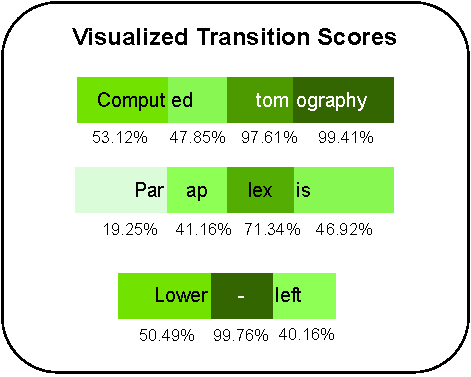
\includegraphics[width=0.65\textwidth]{images/visualized_transition_scores.pdf}}
        \caption{The Alpaca-VQA transition scores visualized.}
        \label{fig:visualized_transition_scores}
    \end{figure} 


    When using the transition scores calculated, the scores can be seen as a decimal value between zero and one. This value can be used as a weight when applying color to each individual token. Some of the predicted answers from \autoref{table:transition_score} are visualized using this method in \autoref{fig:visualized_transition_scores}.

    As transition scores can be useful to get insight into how confident the model is when predicting a token, visualizing the scores can make them more intuitive for a user. Instead of only presenting the transition scores as percentages, colors are more often understood by non-technical users. By making more of the model presentable in an intuitive way, more users can gain insight into how it works and where it can be improved. 
    The next subsection will explain another way to make models more transparent and presentable to humans. The experiment uses a proxy model explained by \gls{lime}. 
    
    
    
    \subsection{Proxy model and LIME}
    \label{sec4:proxy_lime}
    This subsection will describe how the proxy model and \gls{lime} method were adapted to give insight into how the Alpaca-VQA model works.
    
    \subsubsection{Proxy model}
    The proxy model used to interpret the Alpaca-VQA model was trained on the predicted outputs of the \gls{llm}. These answers were generated using half of the available dataset, as shown in \autoref{fig:dataset_split}. The rationale behind this was to see how well the Alpaca-VQA model performed on unseen data that could be used to fit the proxy model so that it mimics the underlying model. 
    The available test set of 20,000 samples with predicted answers by the Alpaca-VQA model was used as a training and testing set for the proxy model. The dataset was split into roughly 70\% training data and 30\% evaluation data. Because a random split was used, the precise numbers used were 14,351 for the training set and 5,649 for the test set.
    The proxy model is a \gls{sdg} classifier implemented by SciKit Learn \cite{SklearnLinearModel}.
    The hyperparameters used when training the proxy model are shown in \autoref{table:proxy_params}. Mostly the parameters used are the default for this implementation of the model, with the most notable difference being that the loss function is a modified Huber instead of the default \textit{hinge}, giving a linear \gls{svm}. 
    The modified Huber is a smooth loss function that brings tolerance to
    outliers as well as probability estimates, and was chosen because it gave the best results among the available loss functions.
    

    \begin{table}[htb]
    \centering
    \begin{tabular}{ r c } 
        \multicolumn{2}{c}{\textbf{\gls{sdg} Classifier Hyperparameters}}\\ 
        \toprule
           Hyperparameter & Value \\
        \midrule
            Loss: & Modified Huber\\
            Penalty: & $L_2$\\
            Alpha: & $1e^{-3}$\\
            Random state: & 42\\
            Max iterations: & 1000\\
            Class weight: & Balanced\\[0.5ex]
        \bottomrule
    \end{tabular}
    \caption{Overview of the parameters used when training the proxy model.}
    \label{table:proxy_params}
    \end{table}
    

    A classification report was made when the \gls{sdg} classifier, used as a proxy model, was fitted. This report can be seen in \autoref{tab:classification_report_proxy}, and it can be seen that the model fits the Alpaca-VQA model with a satisfactory accuracy of 84\%. This score indicates that the proxy model will answer the same as the Alpaca-VQA model approximately 84\% of the time, given the same questions and images.

    \begin{center}
\begin{longtable}{|c|c|c|c|c|}
\caption[Classification Report: Proxy Model.]{Proxy Model Classification Report} \label{tab:classification_report_proxy} \\

\hline \multicolumn{1}{|c|}{\textbf{Class}} & \multicolumn{1}{c|}{\textbf{Precision}} & \multicolumn{1}{c|}{\textbf{Recall}} & \multicolumn{1}{c|}{\textbf{F1-score}} & \multicolumn{1}{c|}{\textbf{Support}}\\ \hline 
\endfirsthead

\multicolumn{3}{c}%
{{\bfseries \tablename\ \thetable{} -- continued from previous page}} \\
\hline \multicolumn{1}{|c|}{\textbf{Class}} & \multicolumn{1}{c|}{\textbf{Precision}} & \multicolumn{1}{c|}{\textbf{Recall}} & \multicolumn{1}{c|}{\textbf{F1-score}} & \multicolumn{1}{c|}{\textbf{Support}}\\ \hline 
\endhead

\hline \multicolumn{5}{|r|}{{Continued on next page}} \\ \hline
\endfoot

\hline \hline
\endlastfoot

0 &   0.87 &  0.98 &  0.92 &   783 \\
1 &   0.00 &  0.00 &  0.00 &   111 \\
2-3mm &   0.00 &  0.00 &  0.00 &     0 \\
3-5mm &   0.99 &  1.00 &  0.99 &    99 \\
Center-left &   0.77 &  0.85 &  0.81 &   336 \\
Center-right &   0.94 &  0.74 &  0.83 &  1,059 \\
Colonoscopy &   0.00 &  0.00 &  0.00 &     9 \\
Endoscopy &   0.67 &  0.94 &  0.78 &   185 \\
Laparoscopy &   0.14 &  0.04 &  0.06 &    60 \\
Lower-right &   0.44 &  0.94 &  0.60 &    98 \\
No &   0.98 &  0.93 &  0.95 &   532 \\
Oesophagitis &   0.00 &  0.00 &  0.00 &     0 \\
Pink &   0.29 &  0.64 &  0.40 &    28 \\
Polyp &   0.97 &  0.77 &  0.86 &   343 \\
Polypus &   0.23 &  0.95 &  0.38 &    22 \\
Red &   0.90 &  0.97 &  0.93 &   178 \\
Upper-right &   0.86 &  0.84 &  0.85 &   784 \\
Yellow &   0.62 &  0.73 &  0.67 &    74 \\
Yes &   0.97 &  0.96 &  0.96 &   893 \\
Biopsy &   0.00 &  0.00 &  0.00 &     1 \\
Endoscopy &   0.45 &  0.30 &  0.36 &    44 \\
Yellow &   0.17 &  1.00 &  0.29 &    10 \\
\hline
Accuracy &  &   &   0.84 &  5,649 \\
Macro average &   0.49 &  0.59 &  0.51 &  5,649 \\
Weighted average &   0.86 &  0.84 &  0.84 &  5,649 \\
 

\end{longtable}
\end{center}


    \subsubsection{Explaining the proxy model with LIME}
    
    In order to interpret this proxy model, the \gls{xai} method \gls{lime} was fitted. Specifically, the TextExplainer module \cite{LimePackageLime} was used to adapt to the proxy model, and the default parameters for TextExplainer were used. The TextExplainer uses as default an exponential kernel that uses a cosine distance metric and only uses words present in the text as explanations. This restriction helps speed up the explanation process, as only the relevant words are used, and not the whole vocabulary of the \gls{llm}. 

    In order to explain the proxy model, the \gls{lime} method first generates a neighborhood of the data by hiding features randomly from the explaining instance. Then the explaining instance uses this neighborhood to learn locally weighted linear models that explain each class. By learning these linear models, the \gls{lime} instance can interpret which word has a high impact on the predicted outcome. 
    
    
    Even though the stacked model design of this explanation pipeline can obscure the underlying Alpaca-VQA model, there are still some insights to be obtained. The \gls{lime} model is designed to give locally accurate interpretations of which parameters the underlying model uses. Therefore, the \gls{lime} model should be transparent to the proxy model. However, the proxy model has no transparency of which features it bases its decisions on. 
    The similarities between the Alpaca-VQA model and the proxy model are that they both are trained on data from the same dataset and sample distribution, with the proxy model ignoring ground truth and using the predicted answer from Alpaca-VQA as its correct answer. 
    Therefore, the proxy model does not give a locally accurate representation of the inner workings of the underlying model and may weigh the inputs differently than the Alpaca-VQA model. 
    Yet, as the proxy model is trained to mimic the underlying model and fits with an accuracy of 84\%, there is still a possibility that the proxy model can give insight into how the \gls{llm} work and possibly exploit biases in the dataset.

    The outcome of the proxy model being explained by \gls{lime} for one instance can be seen in \autoref{fig:lime_crop}. Here it can be seen that the \gls{lime} instance predicts that the input question is most relevant in answering the question. The ground truth answer can be seen in the top left corner of this figure, together with the predicted answer by Alpaca-VQA and the proxy model. In this figure \gls{lime} highlights words that have a high impact on the outcome. The four most probable classes are visualized to the left in the image. The class "Other" is how the \gls{lime} instance classifies the possibility of the predicted class not being in the top four.
    In the \autoref{fig:lime_crop}, it can be seen that the class "Red" is thought to have the highest probability of being correct. In the middle of the figure, the two most probable classes are explained by visualizing the positive and negative impact different words have on the outcome. The figure shows that both "Red" and "Yellow" mostly depend on the same words and do not consider the image features.

    
    \begin{figure}[htb]
        \centerline{
        
\includegraphics[width=1.2\textwidth]{images/LIME_crop.pdf}}
        \caption{The proxy model explained by LIME.}
        \label{fig:lime_crop}
    \end{figure} 

    In this experiment with the proxy model explained by \gls{lime}, there is a likelihood that the model only considers the question and ignores the image features when predicting an answer. Since this is an indicator that the model detected some bias in the language used in the questions, the next experiment removes the image from the input entirely. Testing the Alpaca-VQA model trained on question-answer pairs, including image features, and removing the image features during testing, can provide insight into whether the proxy model exploited the same biases as the underlying model.
    
    


    \subsection{Language-only Alpaca-VQA model}
    \label{sec4_language_only_model}
        
        As noted by the authors of the \gls{vqa} 2.0 dataset \cite{goyalMakingVQAMatter2017}, it could be observed that some \gls{vqa} models in their experiments learned biases in the language of the question-answer pairs. This was demonstrated by removing the image altogether from the testing phase and letting the model predict answers only based on the question. Suppose these language-only models perform similarly to the models that also can see images. In that case, it is an indicator that the model has exploited severe language biases and mainly uses these when answering a question. 
        A model that has exploited these language biases will not ground its answers equally on the question and image, resulting in a reduced ability to answer correctly, given that the same question can have multiple images.

        The classification report on 20,000 language-only test samples is listed in \autoref{tab:classification_report_blind}. The model is the same as in the previous reports, but the images are left out when testing.
        As seen in the classification report, the language-only Alpaca-VQA model has an accuracy of 38\% on this test set. Compared to the model that could also see images, the language-only model managed to correctly classify more samples without analyzing images.

        Generally, a model trained on a larger dataset with more parameters is expected to perform better than one trained on a smaller dataset. This performance is because it has more data to learn from, making it able to capture the underlying patterns in the data more precisely. 
        However, there are certain situations where a model trained on a smaller dataset may perform better, and it is usually related to the quality of the dataset. Because the data quality is different, this performance discrepancy can be why the model trained on language-only performs better than on the complete VQA dataset, including images. 
        
        One possible reason is that the smaller dataset, without image features, may have a higher signal-to-noise ratio, meaning the useful data patterns are more precise and distinct. A dataset with a higher signal-to-noise ratio makes it easier for the model to learn and generalize well to new data. In contrast, a larger dataset with more parameters may have more noise or variability, making it harder for the model to distinguish the relevant patterns. 
        More noise may lead to overfitting or poor generalization performance. In this example, from the loss curve, there is a possibility that the Alpaca-VQA model did not generalize well to the available data, as the graph flattens relatively early in the training phase.
        
        Another possible reason is that the samples with fewer features better represent the target distribution or application domain and may capture the key patterns and characteristics relevant to the task. In contrast, a larger dataset may contain more diverse or irrelevant data that can dilute the important signal and affect the performance of the model. One rationale is that the language-only model's higher accuracy can be explained by the fact that the image features are considered noise to the language model and that it can not utilize the information given.

          
        \begin{center}
\begin{longtable}{|c|c|c|c|c|}
\caption[Classification Report: Language-Only Alpaca-VQA.]{Language-Only Alpaca-VQA: Classification Report on 5,000 question-only samples.\\Model trained on 20,000
question-answer pairs, including images. Tested on only questions.} \label{tab:classification_report_blind} \\

\hline \multicolumn{1}{|c|}{\textbf{Class}} & \multicolumn{1}{c|}{\textbf{Precision}} & \multicolumn{1}{c|}{\textbf{Recall}} & \multicolumn{1}{c|}{\textbf{F1-score}} & \multicolumn{1}{c|}{\textbf{Support}}\\ \hline 
\endfirsthead

\multicolumn{3}{c}%
{{\bfseries \tablename\ \thetable{} -- continued from previous page}} \\
\hline \multicolumn{1}{|c|}{\textbf{Class}} & \multicolumn{1}{c|}{\textbf{Precision}} & \multicolumn{1}{c|}{\textbf{Recall}} & \multicolumn{1}{c|}{\textbf{F1-score}} & \multicolumn{1}{c|}{\textbf{Support}}\\ \hline 
\endhead

\hline \multicolumn{5}{|r|}{{Continued on next page}} \\ \hline
\endfoot

\hline \hline
\endlastfoot


0  &   0.70  &  0.91  &  0.79  &  1,551 \\
1  &   0.57  &  0.51  &  0.54  &  1,132 \\
11-20mm  &   0.30  &  1.00  &  0.46  &    97 \\
2  &   0.00  &  0.00  &  0.00  &   306 \\
3  &   0.00  &  0.00  &  0.00  &    13 \\
4  &   0.00  &  0.00  &  0.00   &  2 \\
5  &   0.00  &  0.00  &  0.00   &  2 \\
5-10mm  &   0.00  &  0.00  &  0.00  &   100 \\
< 5mm  &   0.00  &  0.00  &  0.00  &    55 \\
>20mm  &   0.00  &  0.00  &  0.00  &    71 \\
Biopsy forceps  &   0.08  &  1.00  &  0.15  &    43 \\
Black  &   0.00  &  0.00  &  0.00   &  9 \\
Blue  &   0.00  &  0.00  &  0.00   &  4 \\
Brown  &   0.00  &  0.00  &  0.00  &    10 \\
Cecum  &   0.00  &  0.00  &  0.00  &    33 \\
Center  &   0.00  &  0.00  &  0.00  &  1,121 \\
Center-left  &   0.11  &  0.87  &  0.19  &   831 \\
Center-right  &   0.00  &  0.00  &  0.00  &   861 \\
Colonoscopy  &   0.76  &  1.00  &  0.86  &   761 \\
Gastroscopy  &   0.00  &  0.00  &  0.00  &   242 \\
Green  &   0.00  &  0.00  &  0.00   &  3 \\
Grey  &   0.00  &  0.00  &  0.00  &    16 \\
Ileum  &   0.00  &  0.00  &  0.00   &  2 \\
Injection needle  &   0.00  &  0.00  &  0.00   &  1 \\
Lower-center  &   0.00  &  0.00  &  0.00  &   938 \\
Lower-left  &   0.00  &  0.00  &  0.00  &   616 \\
Lower-right  &   0.00  &  0.00  &  0.00  &   778 \\
Metal clip  &   0.00  &  0.00  &  0.00  &    11 \\
No  &   0.73  &  0.38  &  0.50  &  2505 \\
Oesophagitis  &   0.00  &  0.00  &  0.00  &   240 \\
Orange  &   0.00  &  0.00  &  0.00  &    16 \\
Pale Pink  &   0.00  &  0.00  &  0.00   &  1 \\
Paris iia  &   0.30  &  1.00  &  0.46  &    95 \\
Paris ip  &   0.00  &  0.00  &  0.00  &   101 \\
Paris is  &   0.00  &  0.00  &  0.00  &   125 \\
Pink  &   0.39  &  1.00  &  0.56  &   819 \\
Polyp  &   0.00  &  0.00  &  0.00  &   311 \\
Polyp snare  &   0.00  &  0.00  &  0.00  &    30 \\
Purple  &   0.00  &  0.00  &  0.00   &  1 \\
Pylorus  &   0.00  &  0.00  &  0.00   &  1 \\
Red  &   0.00  &  0.00  &  0.00  &   629 \\
Tube  &   0.00  &  0.00  &  0.00  &   218 \\
Ulcerative colitis  &   0.25  &  1.00  &  0.40  &   250 \\
Upper-center  &   0.16  &  0.14  &  0.15  &   944 \\
Upper-left  &   0.00  &  0.00  &  0.00  &   764 \\
Upper-right  &   0.00  &  0.00  &  0.00  &   729 \\
White  &   0.00  &  0.00  &  0.00  &   520 \\
Yellow  &   0.00  &  0.00  &  0.00  &    79 \\
Yes  &   0.71  &  0.80  &  0.75  &  1,778 \\
Z-line  &   0.28  &  1.00  &  0.44  &   220 \\
brown  &   0.00  &  0.00  &  0.00   &  4 \\
grey  &   0.00  &  0.00  &  0.00   &  7 \\
purple  &   0.00  &  0.00  &  0.00   &  3 \\
\hline
Accuracy &  &  & 0.38 &  20,000 \\
Macro average &  0.10 &   0.19 &  0.11 &   20,000 \\
Weighted average  &  0.31 &   0.38 &  0.31 &   20,000 \\


\end{longtable}
\end{center}

      




\begin{comment}
    DISCUSSION: (some put this as a separate chapter before the conclusion depending on the length of it) It is often also nice to discuss the results in a broader setting, trying to generalize the results beyond the specific case study and selected data. This is often done in a separate discussion section at the end - or if it is a lot to discuss, as a separate chapter. Here, one can also typically include a discussion of challenges and pitfalls experienced, etc.
\end{comment}

\section{Discussion}
\label{4_discussion}
% Intro


% Results in a broader setting



% Proxy model and LIME
As explored in this chapter, visualizing transition scores and having proxy models explained by \gls{xai} methods like \gls{lime} can give insight into how the larger underlying model handles the data. Even though one extra model is stacked on top of the explainability pyramid, it can still provide an understanding of how the model functions. 

An analogy of this proxy model is how most computer vision systems tackle predicting a person's mood by looking at their face. Instead of trying to analyze every facial muscle that makes up the expression, the system looks at the resulting expression when predicting the mood. 
Another example may be how humans can determine the species of trees. As taking a DNA sample every time is relatively resource-intensive, most people use features such as the shape of the leaves, the color, and the structure of the bark. In this example, the \gls{llm} represents the DNA, the proxy model represents the outside of the three, and \gls{lime} represents which features to pay attention to and why these are important. 
Using a proxy model, the \gls{llm} can make a prediction, and some of the details can be abstracted to more high-level features, which can be explained by intuitive methods like \gls{lime}.

In the experiment with the proxy model explained by \gls{lime}, like in \autoref{fig:lime_crop}, it was discovered that the proxy model primarily evaluated the question when predicting an answer. 
This finding was not definite proof that Alpaca-VQA did not evaluate the image features. Still, it highlighted the possibility that the data could be exploited using biases in the linguistic part of the dataset. 

% Language-only
The Alpaca-VQA model, trained on questions and images, was blinded during testing to investigate this finding further. By having the model trained on seeing images, not receiving images, the possibility of it not using the image features could be explored. The model achieved higher accuracy when testing this language-only data than the one tested with questions and images.
This finding suggests that the Alpaca-VQA model trained on the current dataset has learned to exploit linguistic biases, possibly combined with taking advantage of the dataset used being unbalanced. 


% Visualizing transition scores
The transition scores can be calculated by exploring how the \gls{llm} predicts the next token. In the experiments in \autoref{sec4:vis_transtion_scores}, the transition scores were visualized by studying how these scores progress throughout the predicted answer. A user can gain insight into how the model samples from the available distribution of tokens. Further insights about how the model interprets the dataset can be gained by complementing the resulting transition scores with a proxy model. %In conjunction with a proxy model, these insights can give additional insights into how a model interprets the given dataset. 
By leveraging additional models and explanation methods, a user can get a combined interpretation of how larger, more complex, and opaque models may use the available data when predicting outputs.
Another advantage of these additional models and explanation methods is that they require much fewer computing resources than training the primary model. 
This makes these complimentary explanation models have a little-to-no impact during inference, compared to the processing time of an \gls{llm}. 
These explanation methods will, therefore, add additional information on how the model computes an answer, in combination with details on how the model may use the data. These insights can facilitate a user in gaining important information on how the model solves the task.

% Classification Reports
From the classification reports, it could be seen that the Alpaca-VQA model had relatively low accuracy. During the generation of answers, as seen when visualizing transition scores, the model sometimes predicts answers not present in the fine-tuning dataset. This demonstrates the ability of the \gls{lora} implementation to resist catastrophic forgetting, letting the model continue to learn new features without forgetting what has already been learned. 
This prediction of answers not present in the test dataset may be why the model does not achieve higher accuracy. As discussed earlier, another reason for the low accuracy may be that the image features encoded into the input text prompt do not bring more signal than noise to the model. The language-only Alpaca-VQA model did achieve higher accuracy than the one using image features, hinting that the visual elements bring more noise than value into the model. 


% Challenges and pitfalls experienced
Regarding the FLEX-VQA model, although no experiments were conducted using this model, the method still provides a novel take on the VQA task. Using labeled feature maps from a \gls{cnn} to generate supplementary captions to an input image would allow for an explanation grounded in locally accurate features.
As the goal of \gls{vqa} is to answer a question as accurately as possible, it only gives insight into a single instance of how the model interprets the task. The \gls{xai} method \gls{lime} also explains a single, locally accurate sample but can give a global insight into a model by explaining multiple single instances. The way \gls{lime} achieves this global explanation is by utilizing a submodular pick algorithm to isolate instances with non-redundant features. These non-redundant instances are explained by \gls{lime}, and combined, they give a more global understanding of how the underlying model works.
By having the FLEX-VQA model both answer the specific question and supplement with a description of the image, using the locally accurate image features, the model can achieve both a locally accurate and a more global explanation of the image. As the image features are used to make the description, the model uses locally accurate image features to create a descriptive text using natural language that describes the image in a broader way than just answering the specific answer. Given both the answer and the description of a single instance, a user can achieve a complete picture of how the model interprets the task.


 % Summary
\section{Summary}
\label{sec4:summary}
\begin{comment}
    SUMMARY: As mentioned above, the summary section should summarize your achievements, results, etc. Briefly conclude what they mean and what you have learned. 
    No need to lead to the next chapter - the conclusion.
\end{comment}

This chapter presents the results of examining the Alpaca-VQA model, an \gls{llm} designed to answer questions about the contents of images. An investigatory experiment was conducted to see how the model responded to the available dataset. The dataset was modified to remove the majority class to make more of the samples relevant to the specific task.

The Alpaca-VQA model was trained on the larger dataset of 20,000 samples. From the classification report, it could be seen that the model had learned biases in the dataset and potentially exploited biases in the questions. These findings were discovered using explanatory post-hoc methods. Specifically, these methods were a proxy model explained by \gls{lime} and visualizing transition scores of the \gls{llm}. These additional methods gave supplementary information not present in the original model, which helped provide an understanding of how the model may exploit biases in the dataset. 

To explore the possibility of linguistic biases in the model, which could lead to inaccurate or unfair results, a language-only version of the model was tested, and compared its performance to the original version that used both images and language.

The key finding of this research is that larger and more complex models, like an \gls{llm}, can be explained by smaller methods added after the primary model has completed training. These additional models add no significant resources use or compute time during inference but provide valuable insights into the model. In addition, these supplementary models do not change how the larger, more complex model works. Therefore, these models can combine complex methods with layers of explanation that bring valuable insights with no cost to the accuracy of the primary model. 




\chapter{Conclusions}
\section{Summary}
\label{sec:5_1_summary}
\begin{comment}
    Briefly summarize what you have done more or less in a step-by-step manner.
    
    Here you summarize and conclude the thesis, and it contains a lot of repetitions from previous chapters. Often, it has been structured in the following three sections, but sometimes they are also merged (especially the first two).
\end{comment}

% Intro 
This thesis has explored the realm of deep neural networks and the potential ways these can be explained. 
This work has focused on multimodal \gls{vqa} models and how these can be explained in both the visual and linguistic domains.
The \gls{vqa} task has the benefit of being interactive so that a user can input an image and ask a question regarding the contents of the image. Therefore, the model that processes these requests must be a multimodal model that can comprehend both text and images and fuse these to give a correct answer. 


% Method
    Two distinct frameworks were introduced and discussed to provide better explanations and transparency to \gls{vqa} methods.
    % FLEX-VQA
    The first is named FLEX-VQA and combines a robust \gls{vqa} method with the \gls{flex} framework to give locally accurate image descriptions alongside the response to the user's question. 
    This method uses natural language to explain locally accurate and faithful image features.
    An image and corresponding caption are inputted during training and used to find co-occurrences between feature maps of the image network and words in the caption. 
    During interference, the system uses the gradient of the predicted class backpropagated in the \gls{cnn}. The feature maps found in this backpropagation are labeled with the word of highest co-occurrence from the training set and used to generate a natural language description of the image. This ensures that the image description is based on relevant words associated with the predicted class and only features present in the image. This description, faithful to the underlying model combined with a \gls{vqa} task, makes an interactive system where users can ask questions and get informative answers. 
    As this method did not have results, it was discussed in depth so that future works can use it as motivation for new explainable methods.


    % Alpaca-VQA
    The second method described in this work is the Alpaca-VQA model. This is an \gls{llm} in the \gls{llama} family, trained to interpret images and answer questions. As language models by design are usually not multimodal, the image features were extracted using a \gls{cnn}, which then was encoded into the input text. To make this model even more computationally efficient than originally, a \gls{lora} implementation is used. This freezes the weights of the \gls{llm} and only adds a smaller update matrix during training. Using this optimization, the model can learn new tasks without forgetting what it was previously trained on. During interference, the input was put through the original weights and the new update matrix, and the merged result was given as the output. The dataset used was an extensive collection of images from the gastrointestinal tract, paired with questions and answers to each image. 
    \glspl{llm} have no intrinsic or intuitive ways to explain how they interpret the input data or do their reasoning. As these transformer-based architectures continue to outperform other methods and therefore get implemented in new systems, it is vital to be able to interpret their decisions.\\
    
    
% Experiments and Results
    This work investigates how smaller and explainable supplementary methods can be adapted to a larger model to get a more nuanced understanding. 
    The two methods experimented with are visualizations of transition scores and a proxy model explained by \gls{lime}. The proxy model gives insight into which parts of the input data may contribute most when predicting an answer, and the visualization of transition scores provides insight into the model's certainty when estimating a new token. 
    % Transition Scores
    Transition scores extracted during the generation of the \gls{llm}s response give insight into how well the model predicts the token's fit in the sequence. By visualizing these scores, based on the transformer self-attention, a user can get a more intuitive insight into how a sentence is generated. In the experiments, the visualizations provided intuitive insights into the way the model uses prior knowledge from pre-training while providing an assessment of the model's reliability in generating responses.
    
    % Proxy model
    The other method used to explain the Alpaca-VQA model was a proxy model trained to simulate the underlying \gls{llm}. As \glspl{llm} are computationally expensive to run and often challenging to interpret, a model mimicking how the model responds while being explained by \gls{llm} was developed. This model was trained on the responses that the Alpaca-VQA model had given on several image-question-pairs and used the TextExplainer method in \gls{lime} to highlight essential words in making the given prediction. Although the design of a stacked proxy model offers the possibility to obscure the inner workings of the underlying model, it proved useful when investigating how the Alpaca-VQA model used input data.

    With the two explainable post-hoc methods adapted to the Alpaca-VQA model, they could together bring valuable insight into how the underlying model may use the input data. 
    Insights gained from these models indicated that the Alpaca-VQA model seemed to have discovered a bias in the dataset and only evaluated the questions when responding, mostly ignoring the encoded image features. 
    A language-only version of the model was tested to explore if the proxy model and transition scores had uncovered these linguistic biases found by the Alpaca-VQA model.
    The Alpaca-VQA model from the main experiment, trained on both images and text, was given the same test data but with the image features removed. As implied by the supplementary explanatory models, the Alpaca-VQA model utilized biases in the language. This was proven by the language-only model's higher accuracy than the one tested on images and text. 
    As biases in datasets are common, they are sometimes hard to uncover and can lead to inaccurate or unfair results.
    As this finding could have been difficult to discover without these additional explanatory models, they have proven to be valuable in developing a complex system with a model that is hard to interpret at the center without sacrificing accuracy. 

    % Summary
    Through conducting experiments for this study, insights have been gained into the usefulness of post-hoc explanatory models in comprehending larger and more intricate models while maintaining the accuracy that the larger model can offer. 




\section{Main Contributions}
\label{sec:5_3_main_contributions}

\begin{comment}
    Again, you "sell" your work. Convince that you have performed a great piece of research (meaning, stay honest and to the facts, but make sure that all your achievements are listed). What are your main contributions? What have you and the readers learned? What is the main knowledge gained? Put this in the context of section 1.2 - problem statement. 
    Detail out how your research/work answers the initially stated challenges and what the "answers" are. Usually, the main goal/question/objective is repeated and then answered.
\end{comment}
% Main findings

    The goal of this work has been to investigate to what extent explanatory models in different domains can provide additional insights into the underlying data, specifically in the \gls{vqa} task.
    The experiments in this work have proven the ability of post-hoc explanatory models to provide valuable insight into the underlying model with no cost to the explained model's accuracy. 
    The proxy model presents a useful understanding of how the \gls{llm} may work, even though it is not transparent to the underlying model but instead emulates its behavior. The visualization of transition scores provides an intuitive description of how \glspl{llm} predicts tokens in a sequence.  

    In this work, it has been studied how an \gls{llm} can be adapted to a new modality while preserving the knowledge from the pre-training.
    % Additional methods explaining an LLM after training is complete
    This fine-tuned model has then been explained by methods adapted after the training is complete. These smaller, more explanatory methods have given valuable insights and indicators of how the \gls{llm} works on the given dataset. 
    By attaching additional explanatory methods to a fully trained model, the combined solution can leverage all of the initial benefits and accuracy while still providing users with intuitive justifications for its answers. Models that are easier for a user to understand make them more functional and effective for further development.

   


    The key finding of this research is that larger and more complex models, like an \gls{llm}, can be explained by smaller methods added after the primary model has completed training. These additional models add no significant resources use or compute time during inference but provide valuable insights into the model. In addition, these supplementary models do not change how the larger, more complex model works. Therefore, these models can combine complex methods with layers of explanation that bring valuable insights with no cost to the accuracy of the primary model.

    



% Summary
In the experiments carried out in this work, the additional locally accurate explanations proved valuable insights into understanding the model's predictions. Visualizations of transition scores and the proxy model explained through \gls{lime} provided valuable supplementary information that the \gls{llm} initially lacked, contributing to a better understanding of its usage and reliability.



\section{Limitations and Future Work}
\label{sec:5_3_future_work}  % Max two pages

\begin{comment}
    Your thesis will NOT answer everything. Still, it is important that you here show that you are aware of that and list various things that could be done to follow up on your work. What would be the next steps? Next experiments? Maybe link this up against section 1.3 - scope and limitations.
\end{comment}

As the scope of this project limits what can be explored in this work, not every aspect of the methods presented and discussed can be examined. Therefore, in this subchapter, some parts of the limitations of the techniques studied in this work are discussed, and ways to overcome these limitations and further investigate these methods in future research are suggested.

\subsection{FLEX-VQA}
    % Limitations
    The FLEX-VQA model presented in this work did not provide any results due to technical issues outside the scope of this work. However, the method offers a solution for a better understanding of the methods used in critical computer vision systems deployed today.

    % Future work
    Some initial issues have been solved when developing this model, but some remain to be overcome. The most prominent remaining problems have been discussed in  \autoref{subsec:no_flex}. Most notable is to make the \gls{flex} framework non-dependent on the machine learning framework Caffe. As this framework is no longer developed, its support for modern hardware and complimentary software dependencies is decreasing. The \gls{flex} framework still possesses the potential of making systems dependent on \glspl{cnn} more transparent to its users. Therefore, future research is encouraged to develop this method further and other variants of locally accurate post-hoc methods. 

    % making FLEX run
    In future research, the \gls{flex} framework should not build its dependence on Caffe for this method to be implemented efficiently and with versatility.
    This adaptation can be made in a multitude of ways, where the main goal would be to decouple the \gls{cnn} feature extraction from \gls{flex}. Modern machine learning frameworks have properties that easily traverse networks and list their feature maps. This allows for a more manageable implementation of \gls{flex} that can be agnostic of the specific \gls{cnn} model used. 


    % Transformers and FLEX
    One restriction of the current implementation of \gls{flex} is that it is based on explaining \glspl{cnn}. Most computer vision systems today rely on \glspl{cnn} as the algorithms window to the outside world. 
    Transformer-based vision systems are, however, gaining popularity and are used instead of \glspl{cnn} in many modern systems. As the current state of \gls{flex} depends on labeling \gls{cnn} feature maps, it does not currently work with other vision algorithms. The \gls{flex} framework may still be adapted in future work to the transformer architecture, as the main requirement is that it can map specific features in the input to particular parts of the internal features. Various methods have been developed to explain transformers more transparently. Many of these rely on a GradCAM method or similar methods based on heat-maps of gradients \cite{barkanGradSAMExplainingTransformers2021, cheferTransformerInterpretabilityAttention2021}.
    These heat-map-based methods can, in theory, be used to map specific labels to the gradients and relevance matrices throughout the computation, resulting in a locally accurate representation of these matrices. By labeling these features with co-occurring words, \gls{flex} can be used to generate descriptive captions using the locally accurate features of the transformer.
    
    A limitation that could be solved by adapting \gls{flex} to a transformer is more accessible transfer learning compared to \glspl{rnn}. Currently, the \gls{flex} framework needs a dataset containing image descriptions and a single class label. The class label is used to train the \gls{cnn} to predict the class, and the image description is used to train the \glspl{lstm} to output the locally accurate description. Not many datasets are available with both these features, so the transformer could be pre-trained using image descriptions to label its gradient features. \gls{flex} can then label features in the gradients before the transformer is fine-tuned on the specific task. Although the development of this method uses \gls{flex} in between transfer learning and does not become fully post-hoc, it does not affect the fine-tuned model. Therefore, it still contains the same benefits of allowing the finished model to train and interpret uninterrupted while providing transparency.


\subsection{Alpaca-VQA}

% Limitations and Future Work

    % No fine-tuned cnn
    One constraint of the implemented Alpaca-VQA model is that it uses a \gls{cnn} not pre-trained for the given task. It may not be a robust approach depending on the fact that the feature maps of the pre-trained classes from ImageNet are similar to the ones observed in separate tasks. 
    Future work can include fine-tuning the \gls{cnn} used for the specific task, making the extracted image feature more relevant. 
    The \gls{cnn} used in future works is encouraged to experiment with object detection models that can encode \gls{roi} or bounding boxes so that the \gls{llm} can learn to interpret where the objects are in the image.

    % Bad accuracy on the experiments conducted in this thesis.
    % The LLM may not be the best fit for the dataset used. 
    % Fine-tune an LLM to a medical dataset that could be combined with a vision-LLM
    In the experiments conducted in this work, the goal has not been to train a state-of-the-art \gls{llm}, but rather explore how it can be explained. This is reflected in the relatively low accuracy for Alpaca-VQA on the given dataset.
    However, in future experiments, \gls{llm} could be extended to make it more beneficial to the end user.
    An interesting future work could include an \gls{llm} pre-trained on domain-specific data, like a medical dataset, before fine-tuning to include images. This way, the system user could ask questions about an image or simply text-only questions. Therefore, the \gls{llm} could be used as a multimodal personal assistant in a domain-specific setting. 

    % It does not answer the questions using natural language.
    The Alpaca-VQA model used in this work is trained to output only the predicted answer to a question to facilitate evaluation. However, this does not use the ability of \gls{llm} to construct sentences in natural language. Because the model is pre-trained on instructions-following tasks, it can still generate longer responses. Techniques such as self-instruct, also used when generating data for the Stanford Alpaca model, can make datasets with natural language answers. Future work can use these methods to create a dataset containing descriptive information in natural language based on factually correct information. 

    % Step-by-step reasoning
    % Interesting results were investigated in previous work by asking \glspl{llm} to answer step-by-step, also called chain-of-thought \cite{lievinCanLargeLanguage2023, weiChainofThoughtPromptingElicits2023}. This prompt engineering causes the model to output its thought process, allowing users to follow their reasoning. The Alpaca-VQA did not respond to this prompt, most likely due to its relatively few parameters compared to other \glspl{llm}. However, it has been found that by training with more data, \gls{llama} models achieve comparable results to larger models \cite{touvronLLaMAOpenEfficient2023}. Future research on step-by-step prompting in multimodal models could provide valuable insights into how \glspl{llm} works.
    

\subsection{Explainable Methods}

% Limitations and Future Work
    The experiments in this work have demonstrated how smaller, more transparent models can be adapted to explain a more complex and opaque model. 
    However, the models described in this thesis have some limitations. 
    % Self-Attention may not be accurate to the decisions made by the model
    One of these is that the visualization of transition scores and self-attention are unreliable sources of insight into how the model works. 
    Some previous works have investigated how attention may not be an interpretable nor accurate method to explain methods based on attention \cite{serranoAttentionInterpretable2019, jainAttentionNotExplanation2019}. 
    As presented in this work, these features can still bring valuable insights into how the model work and interprets the data. 
    Therefore, a future experiment worth investigating would be a larger user study, asking end users whether attention or transition scores make a model more intuitive.
    
    % The proxy model is not transparent to the underlying LLM
    The proxy model used in this work had the limitation that it was not transparent how the Alpaca-VQA worked. It was designed to simulate the behavior of the \gls{llm} instead of giving direct insight into how the underlying model functioned. Yet, during experimentation, it provided valuable insights that helped discover bias in the Alpaca-VQA model. 
    As more complex models get higher accuracies at the cost of transparency, future work is needed to develop models with intrinsic explainability or methods that can be attached to a larger model post-hoc.\newline

    % Some smart end sentence here

    
    In summary, this thesis has explored powerful \gls{ai} methods on the \gls{vqa} task using \glspl{cnn} and \glspl{llm}, highlighting the inherent challenges in comprehending their underlying reasoning. This work has made noteworthy progress by investigating various techniques for increased transparency. 
    However, it is important to acknowledge that there is still much more to be done in the field of \gls{xai} as research strives towards achieving a deeper understanding of these complex systems.



\backmatter{}
\singlespacing
\printbibliography

\end{document}
